\section{Experiments}

To understand in which scenarios the inclusion of shape constraints is beneficial, a series of experiments was conducted.

The final implementation was done in the programming language \texttt{Python} using the \texttt{GPyTorch} library \cite{Gardner2021}, and it is available at \url{https://github.com/adamesalles/shape-constrained-gaussian-processes}, which also contains the results of the experiments conducted.

The choice of \texttt{GPyTorch} was due to its ability to perform operations efficiently on a GPU (using Nvidia CUDA), which is essential for large-scale experiments and numerical hyperparameter optimization. Initial prototypes were developed in \texttt{Julia} with the \texttt{GaussianProcesses.jl} library~\cite{Fairbrother2022} and in \texttt{R}~\cite{R} with the \texttt{GPfit} library~\cite{GPfit2015}.

The experiments were conducted on a Ryzen 7 5800H (8 cores, 16 threads) with 24GB of RAM and an Nvidia RTX 3050 GPU with 4GB of video memory.

\subsection{Normalized Power Prior}

The initial application planned for the developed methods is the emulation of functions in noisy Monte Carlo Markov Chain (MCMC) settings.
In this context, a relevant example in the literature is the emulation of models using the \textit{Normalized Power Prior} (NPP) \cite{Carvalho2021}.

% \comLM{State that $f_{z}(\alpha)$ is strictly convex when $\pi$ is proper.}

Consider a tempered posterior distribution of the form \( p_{\alpha}(\theta \mid \bfz) \propto l(\bfz \mid \theta)^\alpha\pi(\theta) \) for \( \alpha \in [0, 1] \).
Our goal is to emulate \( f_{\bfz}(\alpha) = \int_{\Omega}l(\bfz \mid t)^\alpha\pi(t)\, \mu(\mathrm{d}t) \) with \( M = 20 \) noisy evaluations, which are computationally costly.
In the case where the prior distribution is an NPP and also proper, the function \( f_{z}(\alpha) \) is strictly convex in \( \alpha \).

The datasets used in the experiments are the four combinations of:

\begin{itemize}
    \item HC and MC (\textit{high curvature and medium curvature}): representing the curvature of the function \( f_{\bfz}(\alpha) \).
    \item \textit{uniform} and \textit{adaptive}: the evaluation grid is either regular or irregular, using the algorithm \ref{alg:bisection-type}.
\end{itemize}

\subsection{Comparison between Gaussian Process and SCGP}

In this section, we compare the fit of the traditional Gaussian Process with that of the SCGP in high and medium curvature scenarios, evaluated on regular and irregular grids.
There are two experiments, assessing the fit capabilities of the proposed methods under variations in curvature and the position of observed values, while reducing the number of observed points.

\subsubsection{Variations in Curvature and Position of Observed Values}
\label{sec:curvature}

Our first experiment consists of evaluating the fitting ability of the proposed methods under variations in the curvature and position of observed values.

For the regressions in these \( M=20 \) evaluations of \( f_{\bfz}(\alpha) \), we used the Radial Basis Function (RBF) as the kernel function \( k \) and \( m(x) = 0 \) as the mean function.
Additionally, for hyperparameter optimization, we used the Adam optimization method \cite{Kingma2017} with a learning rate of \( 10^{-2} \), 1000 iterations for the GP, and 2000 iterations for the SCGP. The MSE is evaluated on a grid of 1000 uniformly spaced points.

In the case where curvature is medium and evaluations are done on a regular grid, \zcref{fig:uniformMC} shows the comparison between Gaussian Process with and without shape constraints under medium curvature.

\begin{figure}[H]
    \centering
    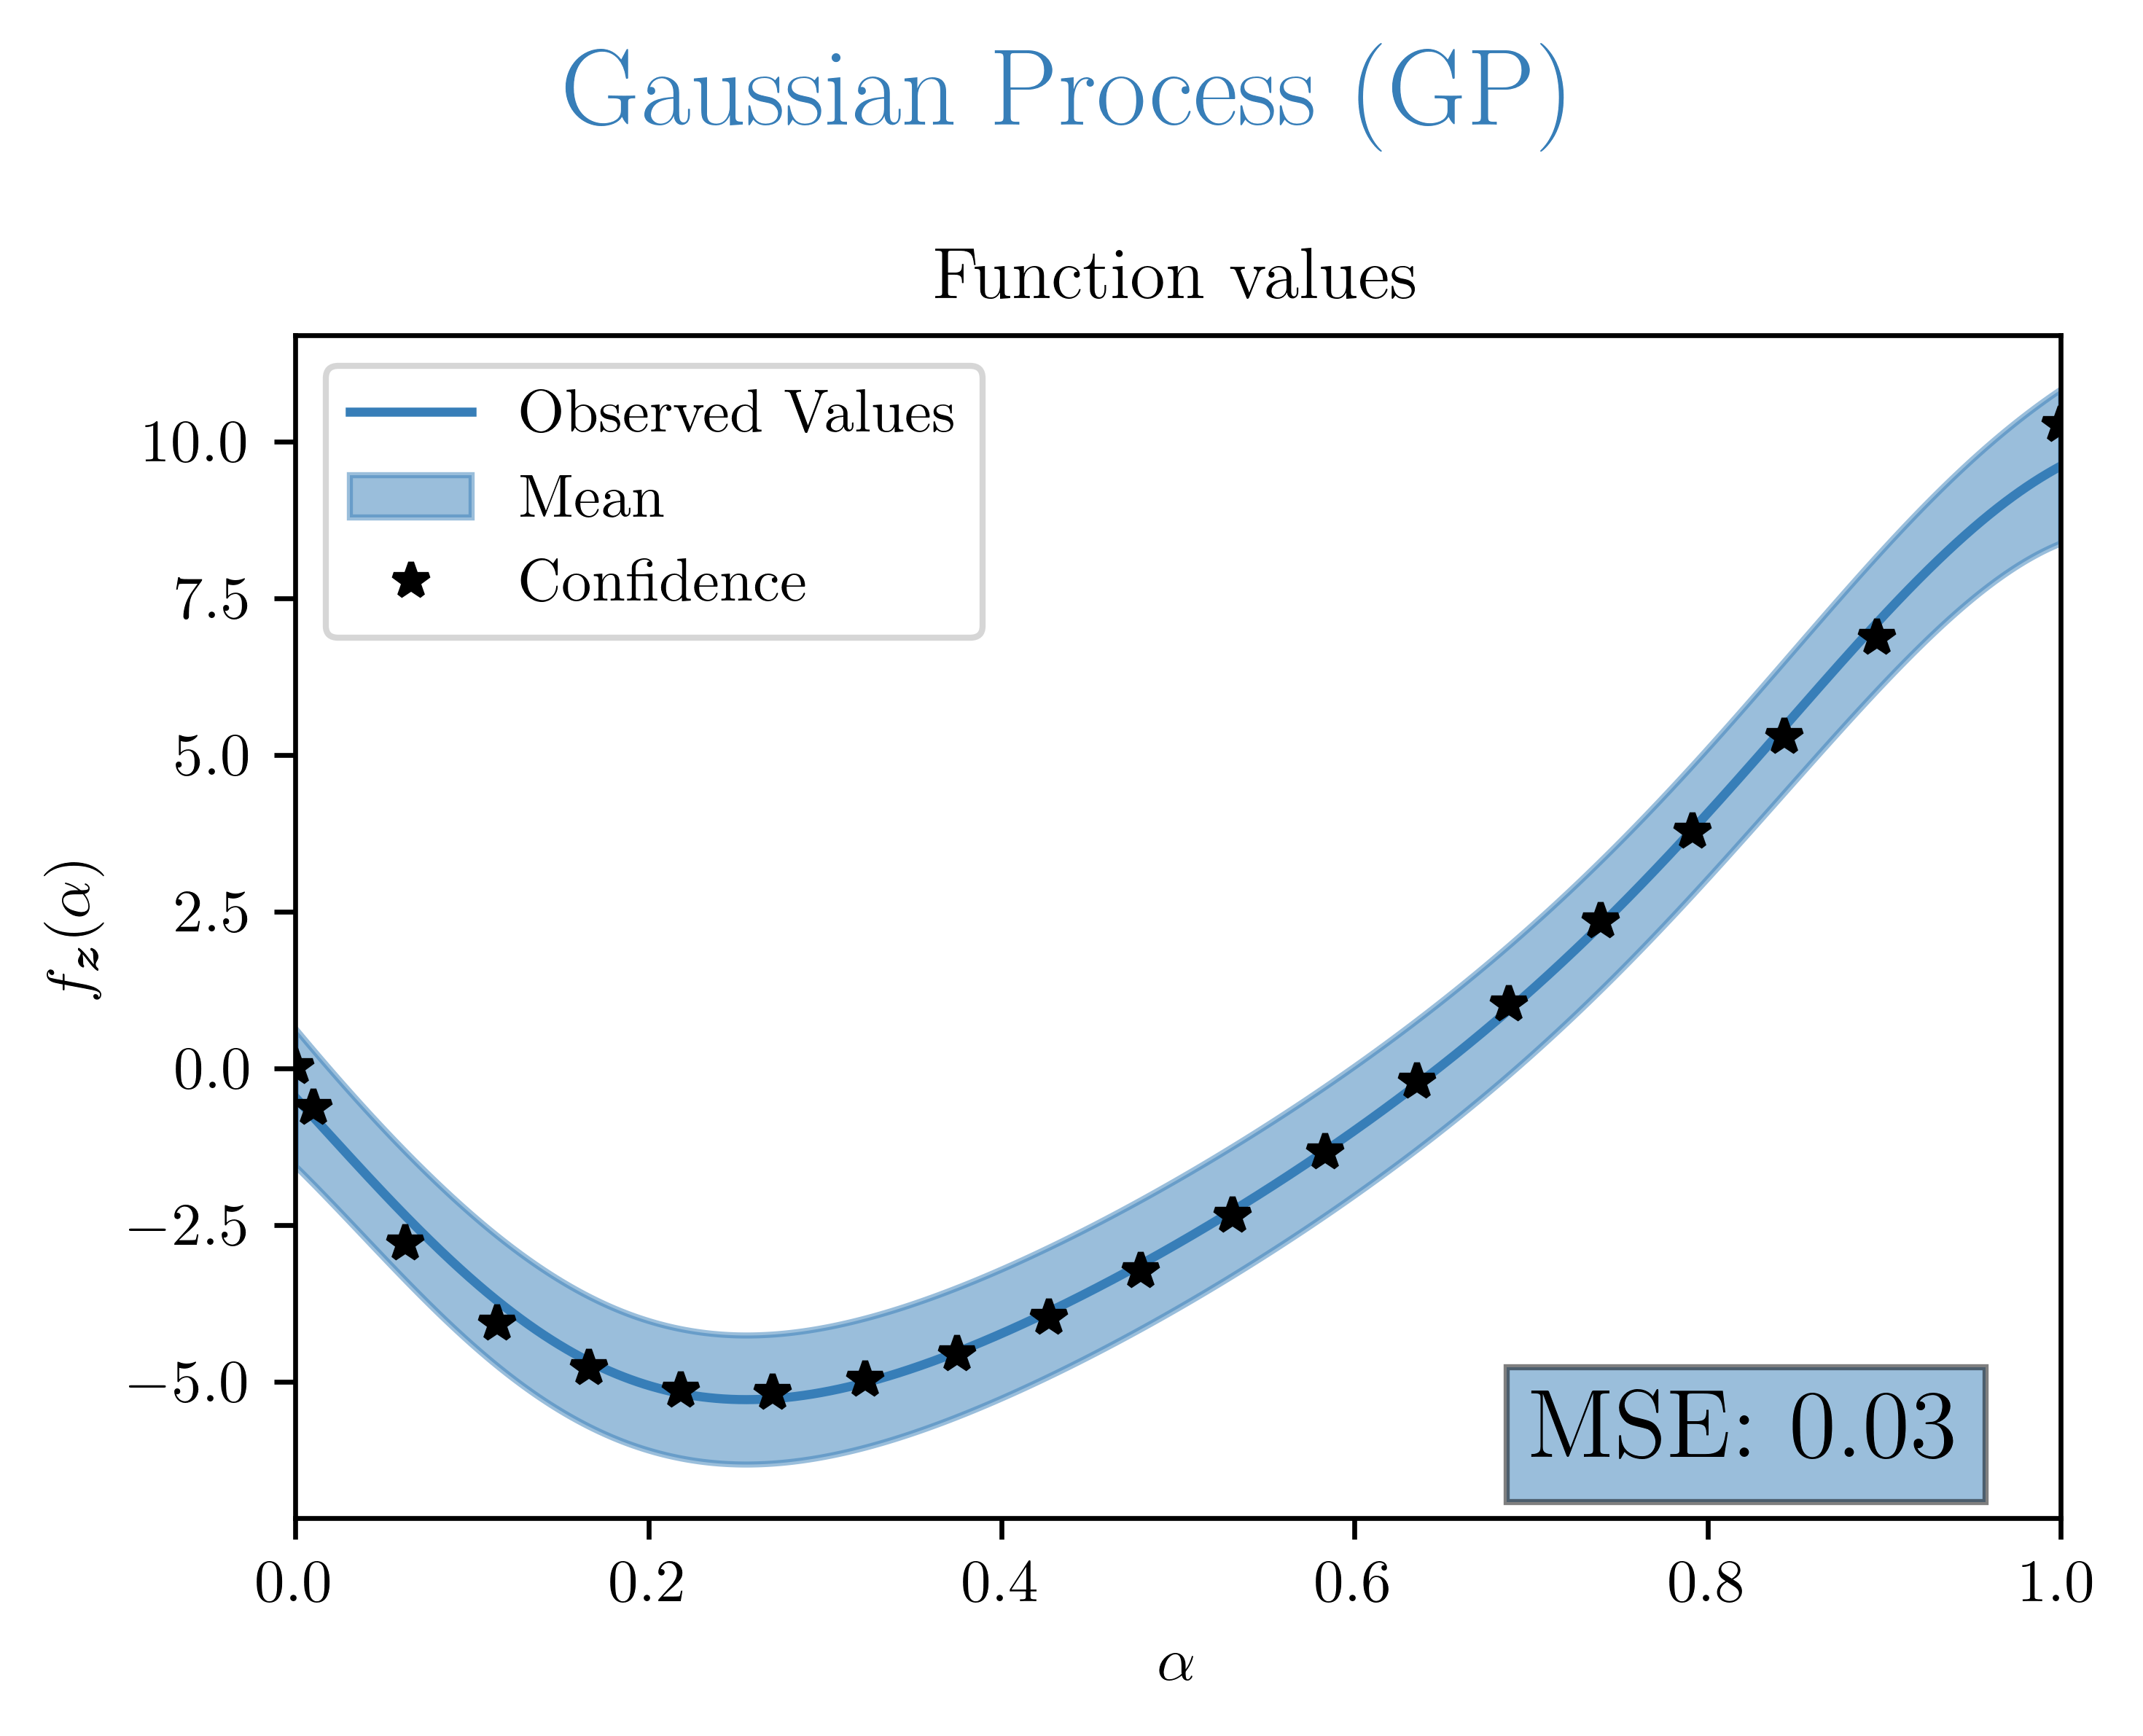
\includegraphics[width=.33\textwidth]{../experiments/uniform_new_MC/GP_20_nobs.png}
    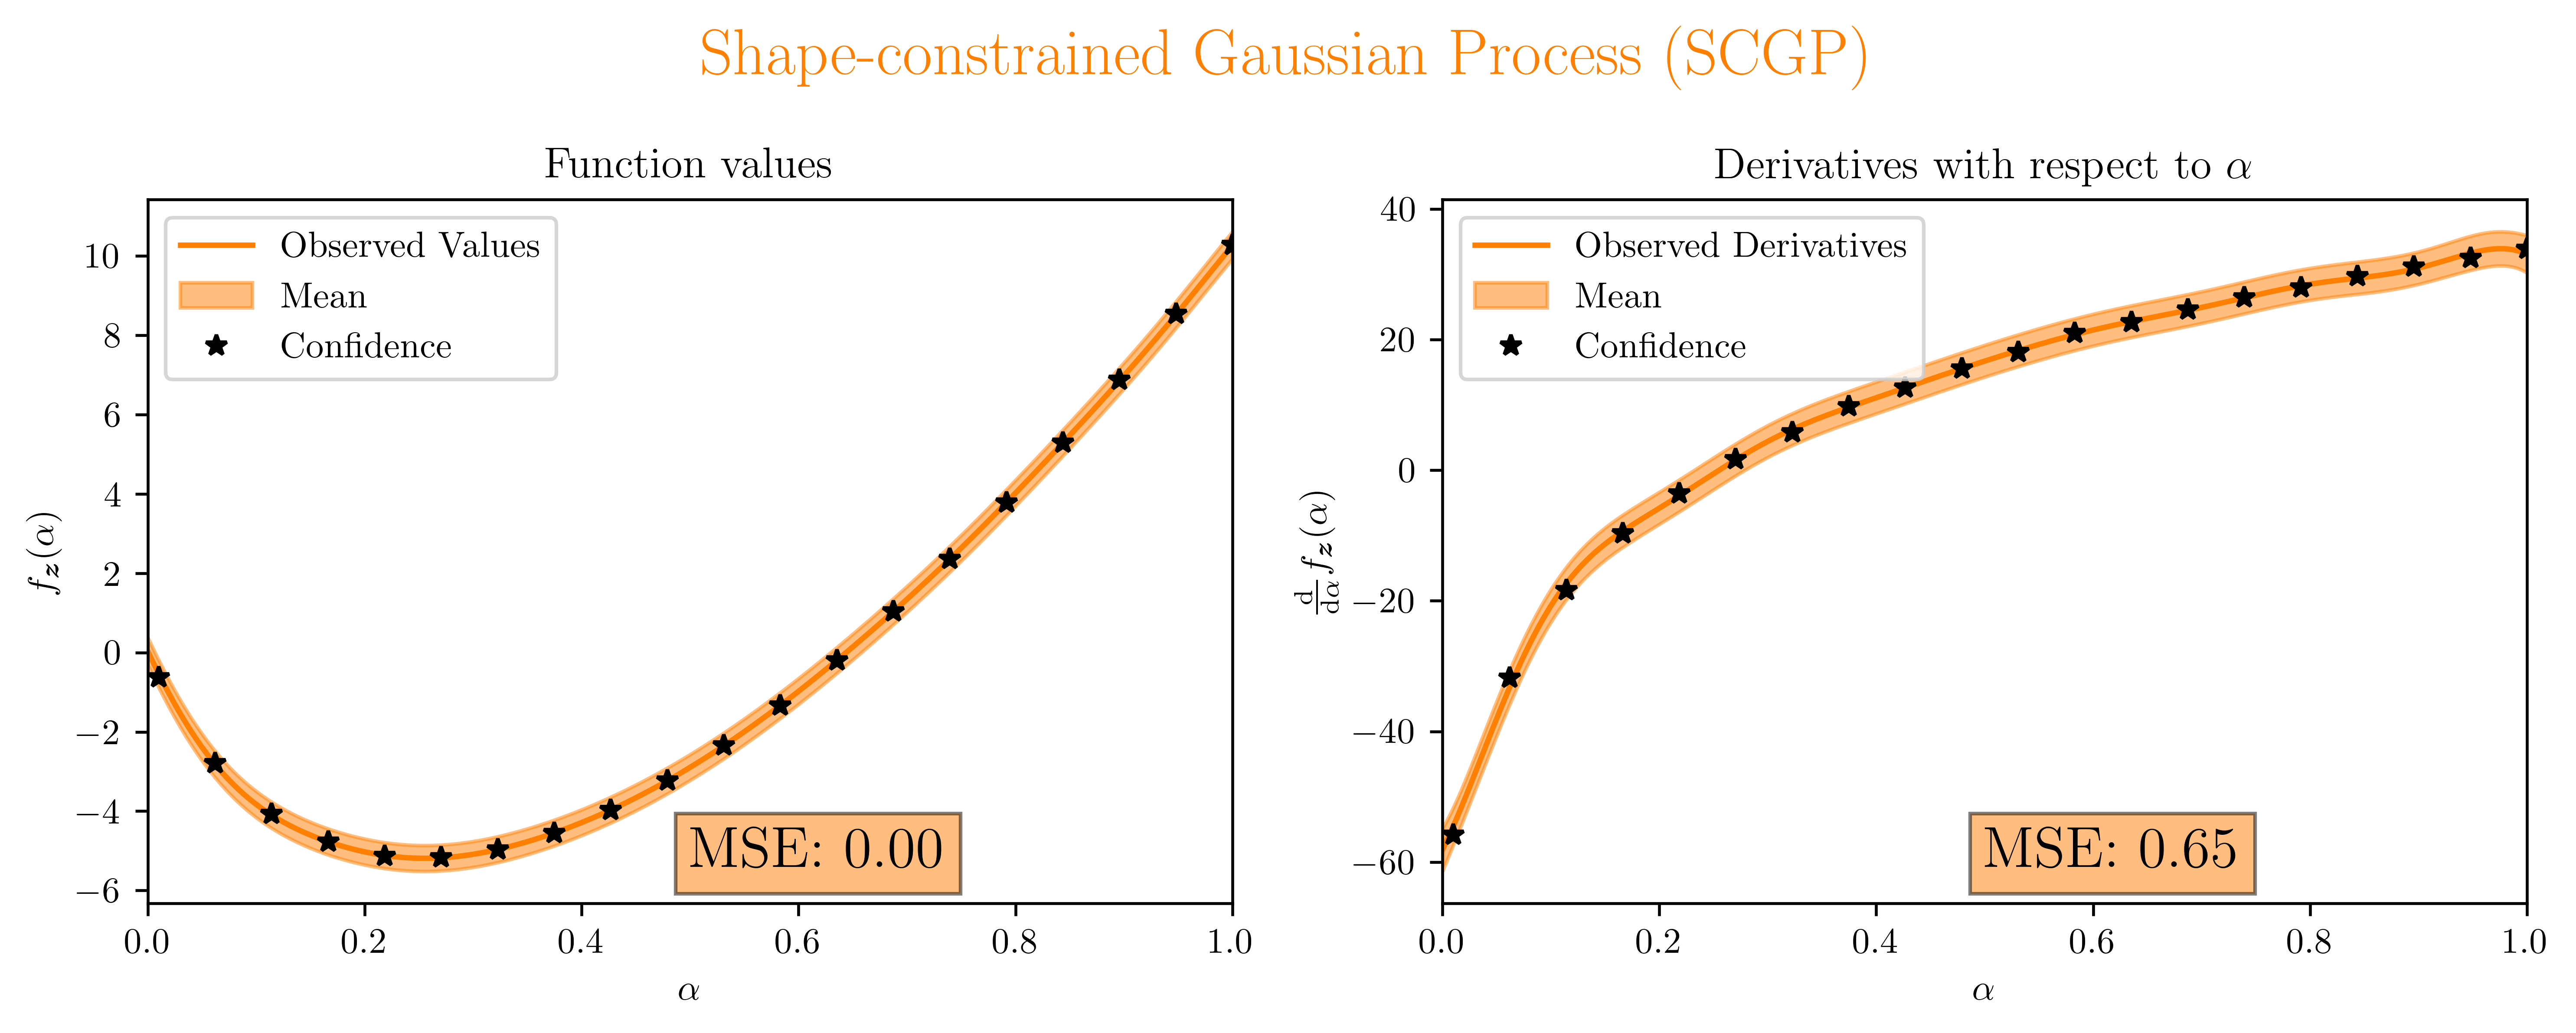
\includegraphics[width=.66\textwidth]{../experiments/uniform_new_MC/SCGP_20_nobs.png}
    \caption{ {\small Comparison between Gaussian Process with and without shape constraints under medium curvature and regular grid evaluation. Source: author.}}
    \label{fig:uniformMC}
\end{figure}

It can be observed that the Gaussian Process with shape constraints is able to capture the curvature of the function \( f_{\bfz}(\alpha) \) more accurately, while the Gaussian Process without shape constraints tends to underestimate the curvature.

\begin{obs}
    Note that the derivative process fitting was satisfactory, which will be important in future experiments. The comparison, however, should be made between the functions \( f_{\bfz}(\alpha) \) rather than between the functions \( f_{\bfz}^\prime(\alpha) \).
\end{obs}

In the case where evaluations are done on an irregular grid, \zcref{fig:adaptiveMC} shows the comparison between the methods. In this scenario, the SCGP correctly captures the shape constraint, while the traditional GP disregards the convexity of the function. However, both methods show a less satisfactory fit.

\begin{figure}[H]
    \centering
    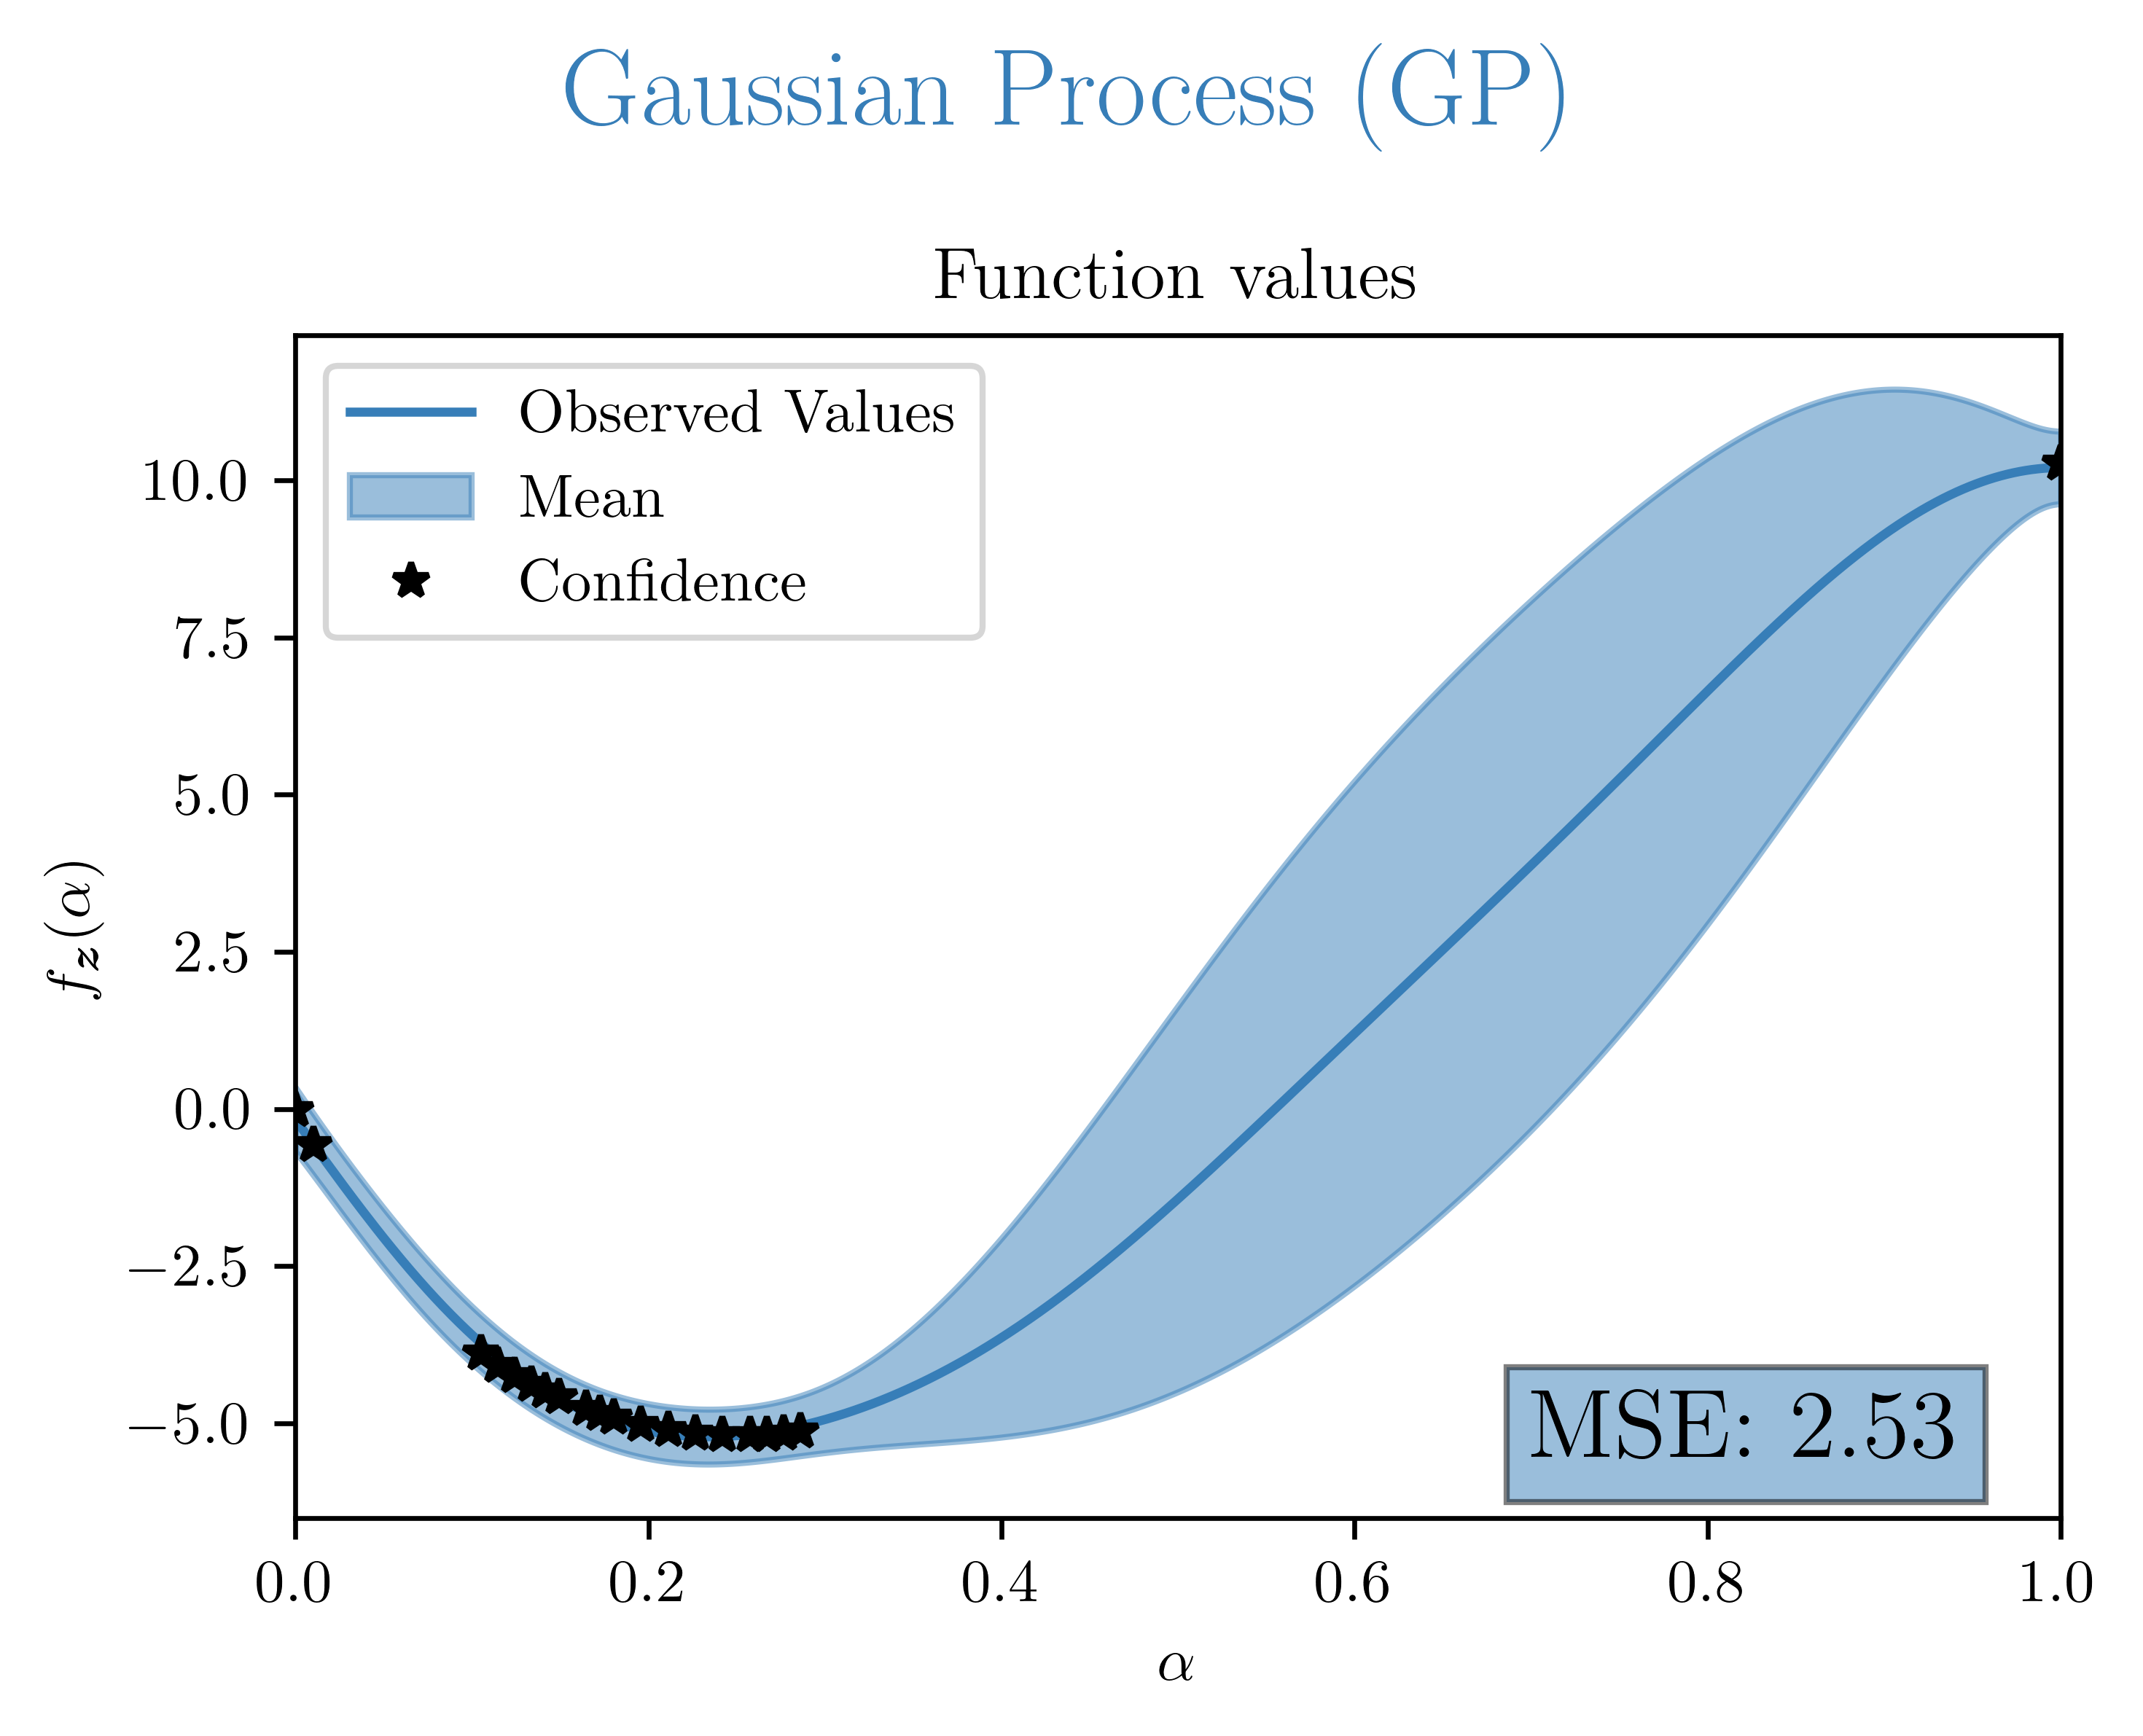
\includegraphics[width=.33\textwidth]{../experiments/adaptive_new_MC/GP_20_nobs.png}
    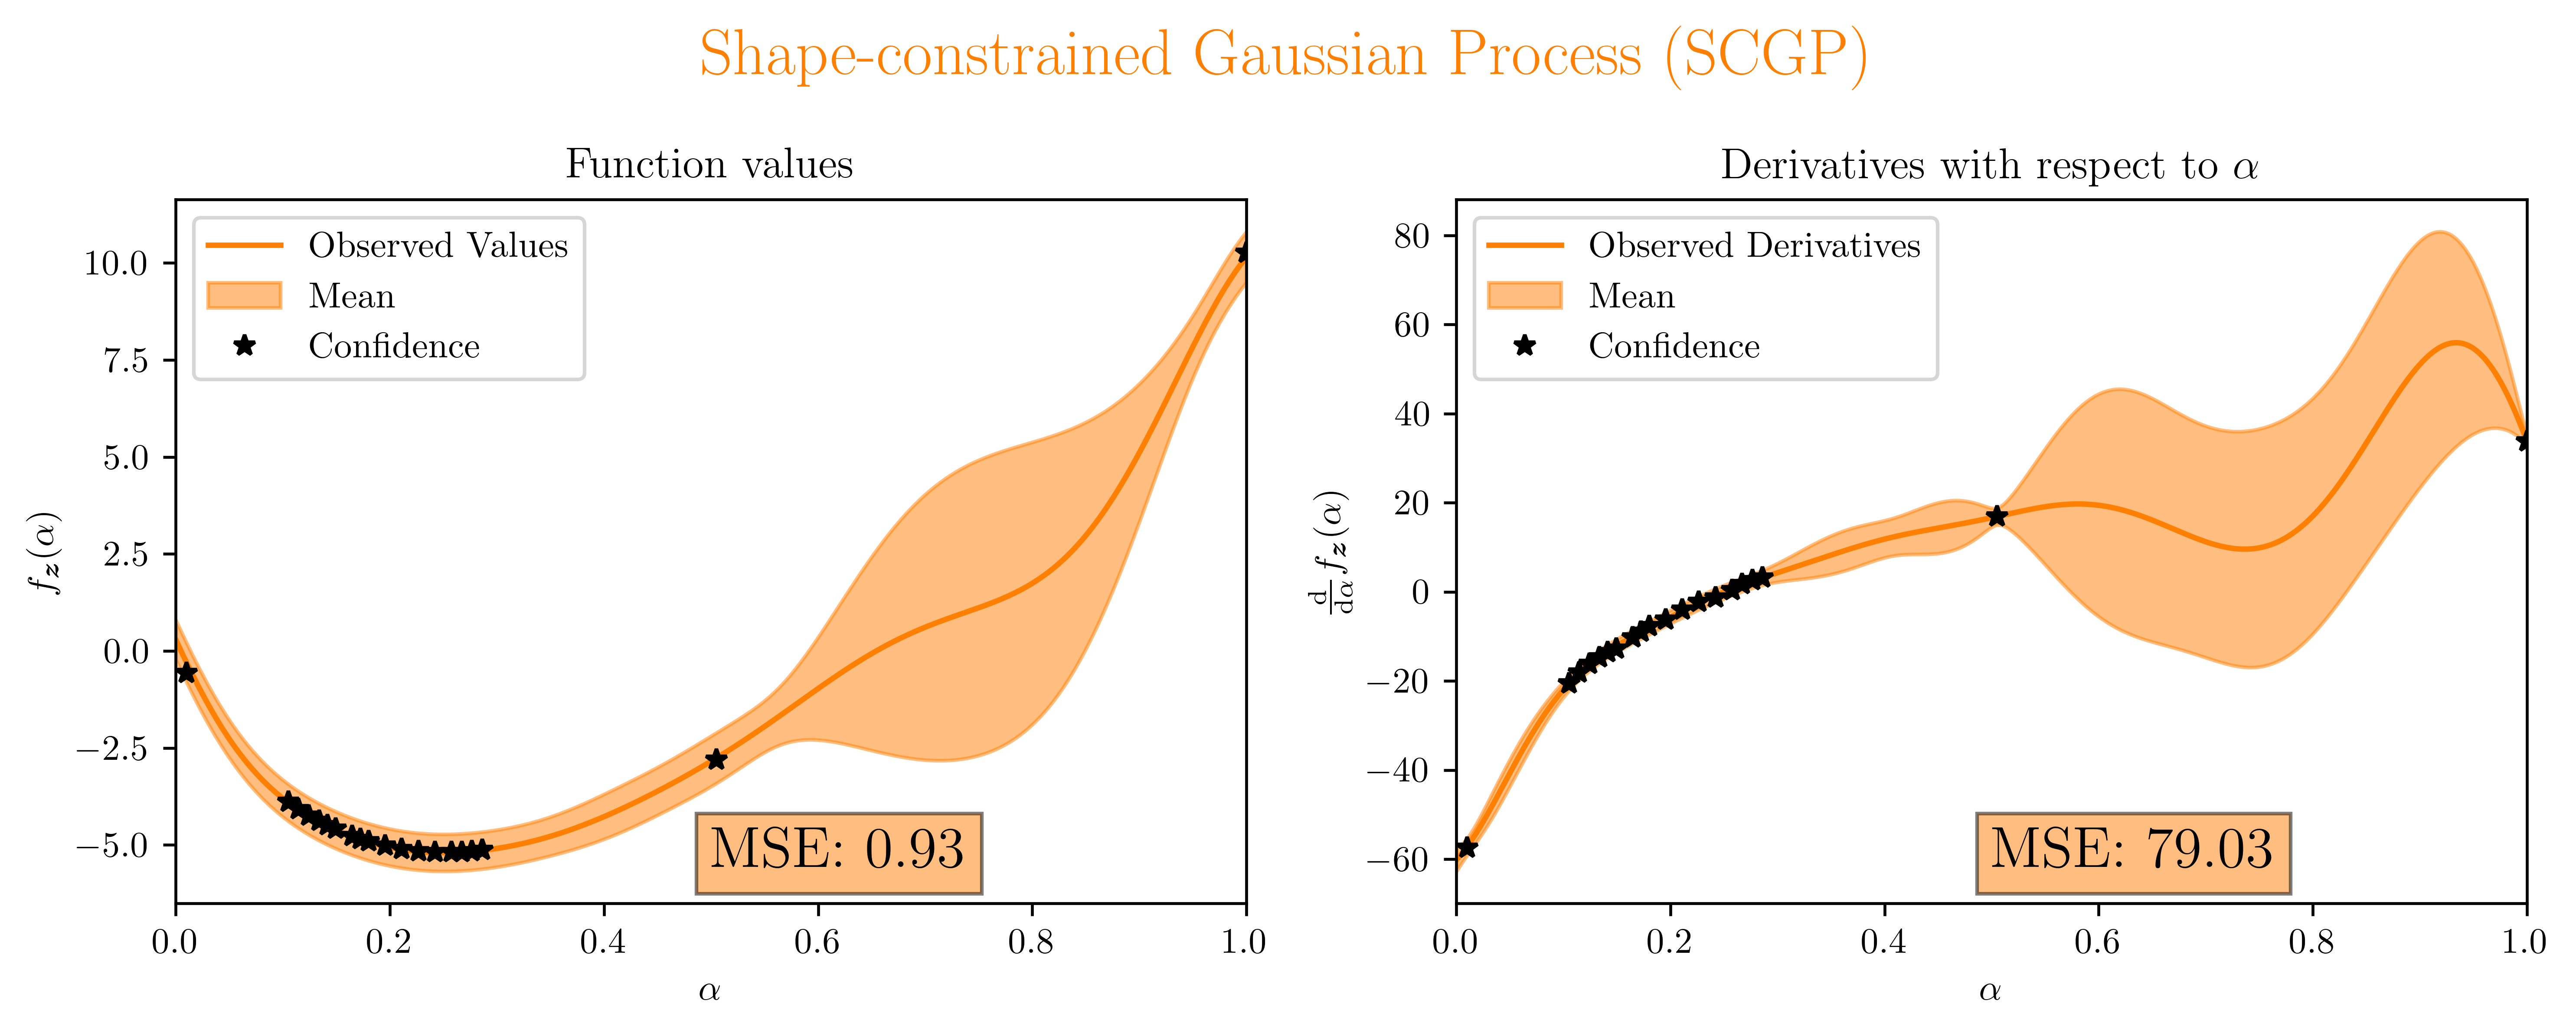
\includegraphics[width=.66\textwidth]{../experiments/adaptive_new_MC/SCGP_20_nobs.png}
    \caption{ {\small Comparison between Gaussian Process with and without shape constraints under medium curvature and irregular grid evaluation. Source: author.}}
    \label{fig:adaptiveMC}
\end{figure}

Evaluating the high curvature scenario, \zcref{fig:uniformHC} shows the comparison in the high curvature scenario with regular grid evaluation. In this case, the SCGP is much better at capturing the curvature of the function \( f_{\bfz}(\alpha) \) compared to the traditional Gaussian Process.

\begin{figure}[H]
    \centering
    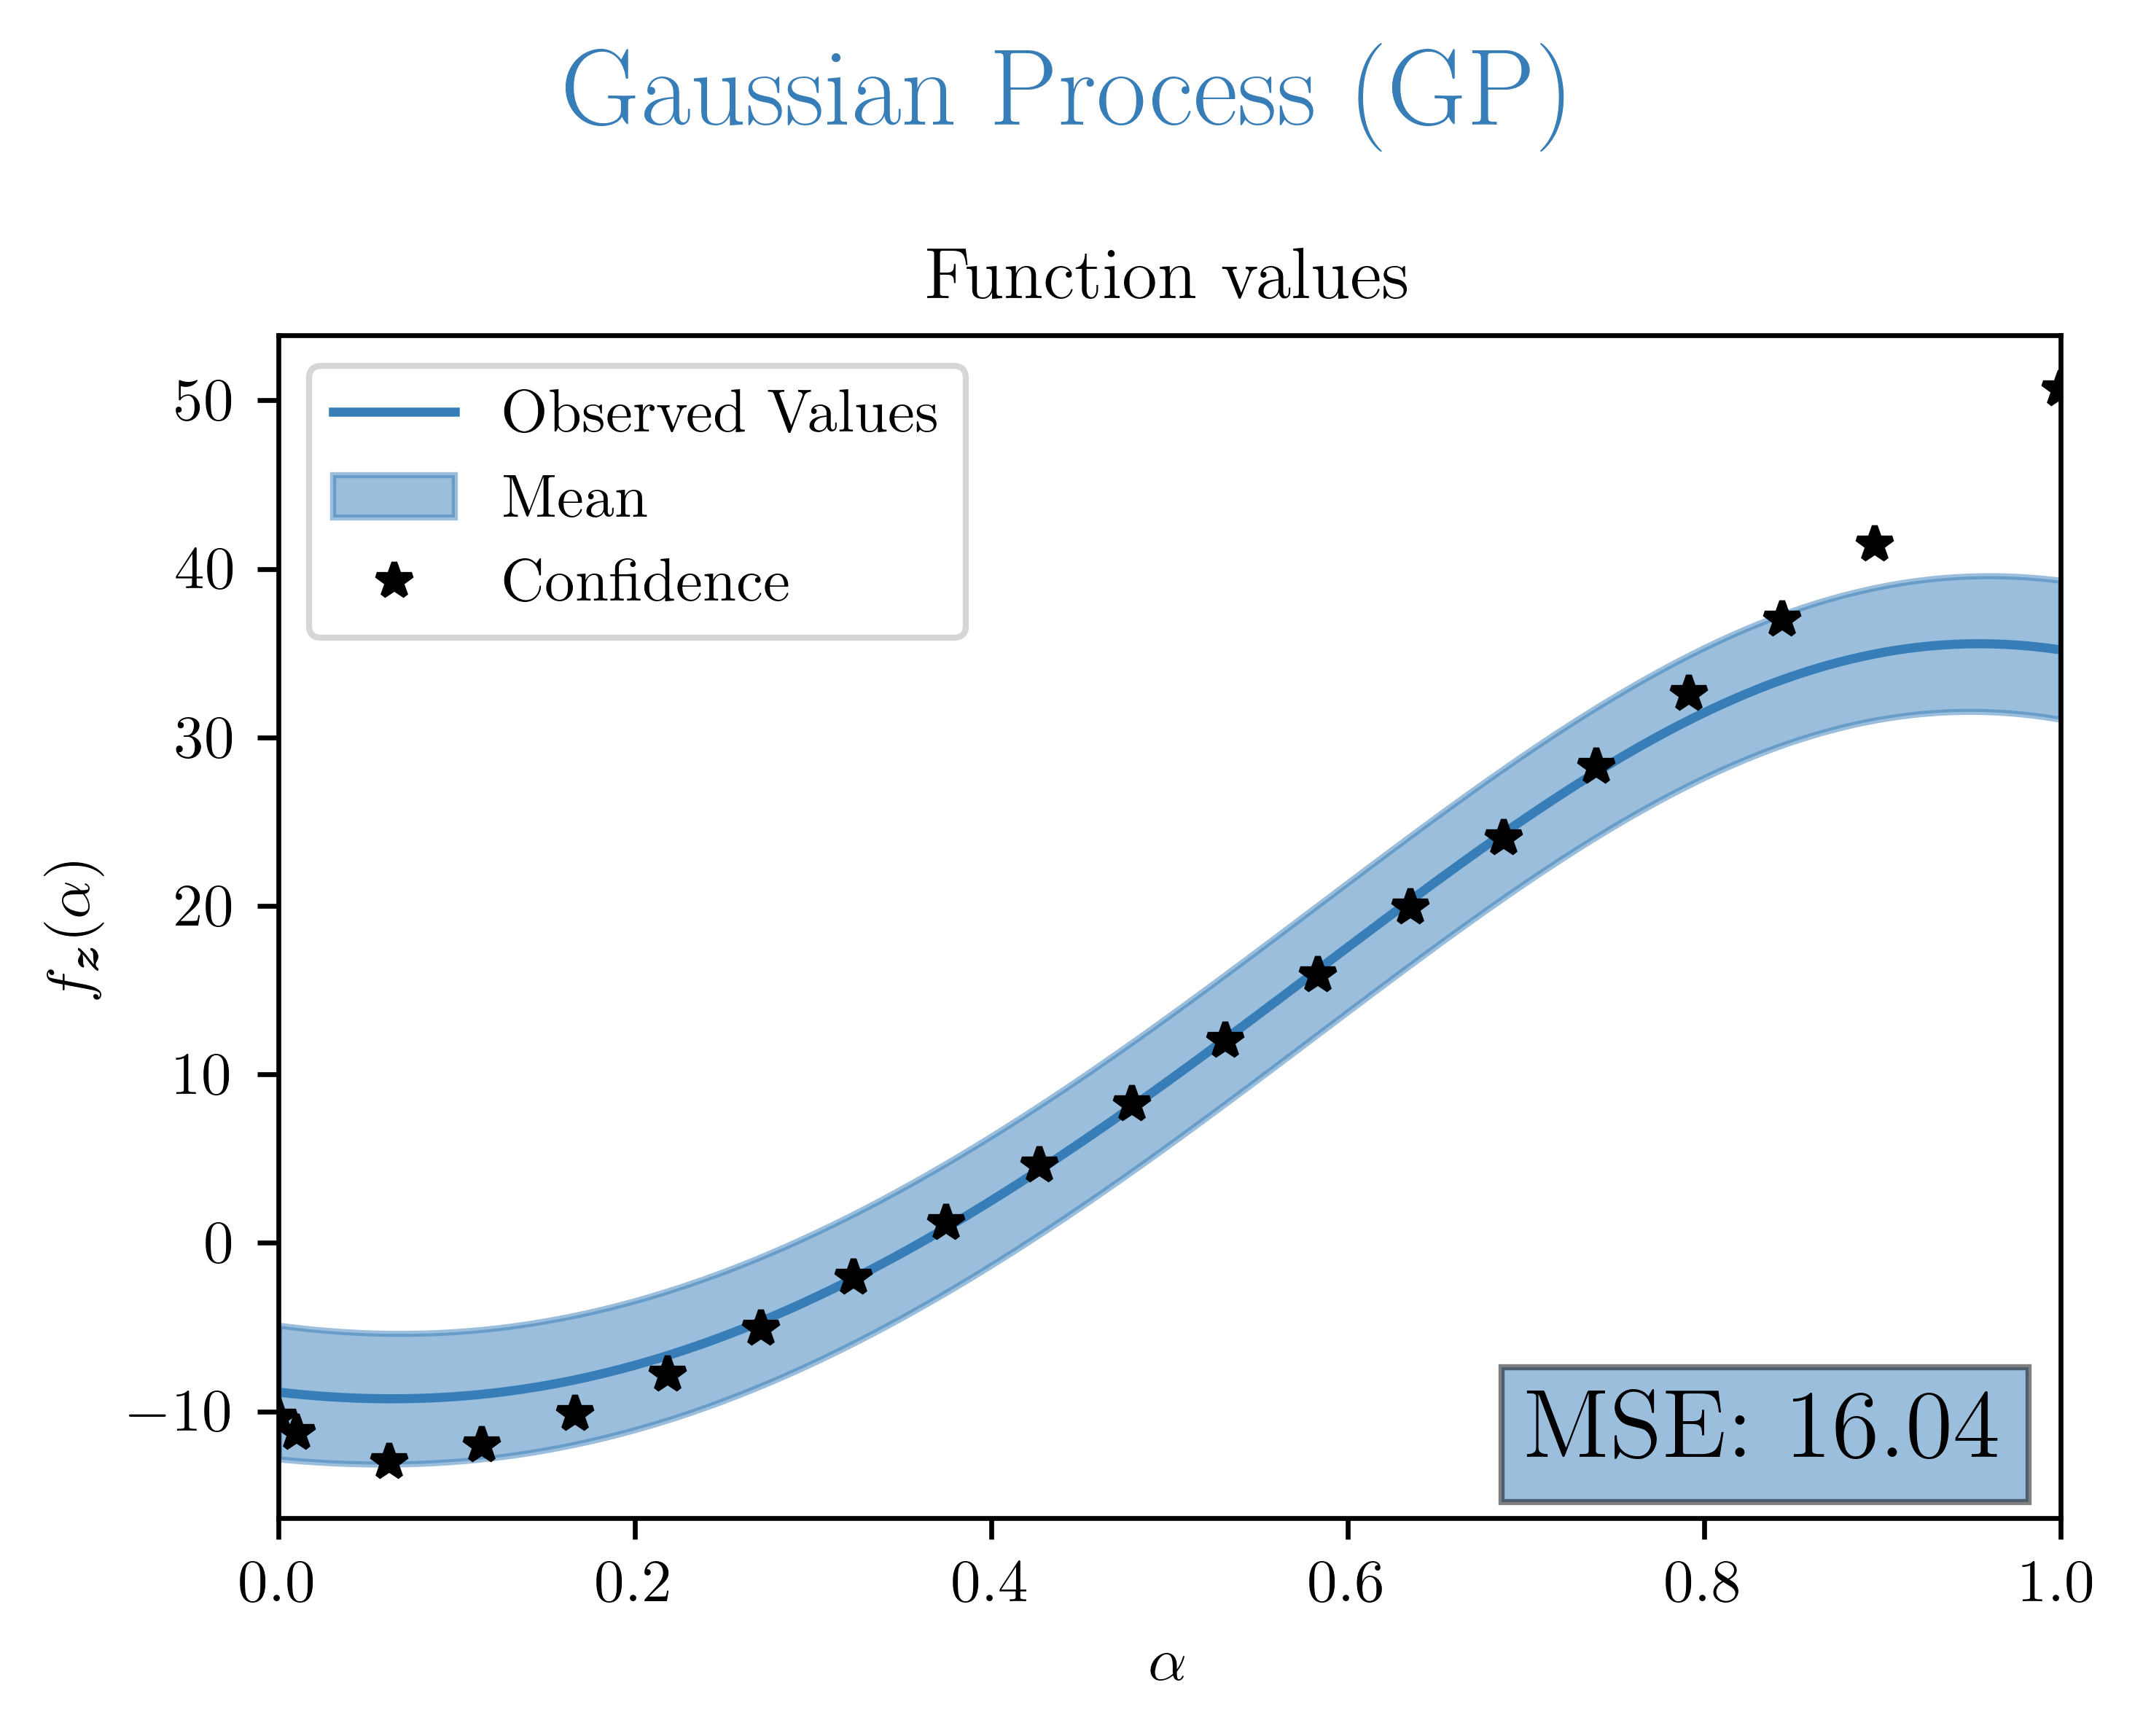
\includegraphics[width=.33\textwidth]{../experiments/uniform_new_HC/GP_20_nobs.png}
    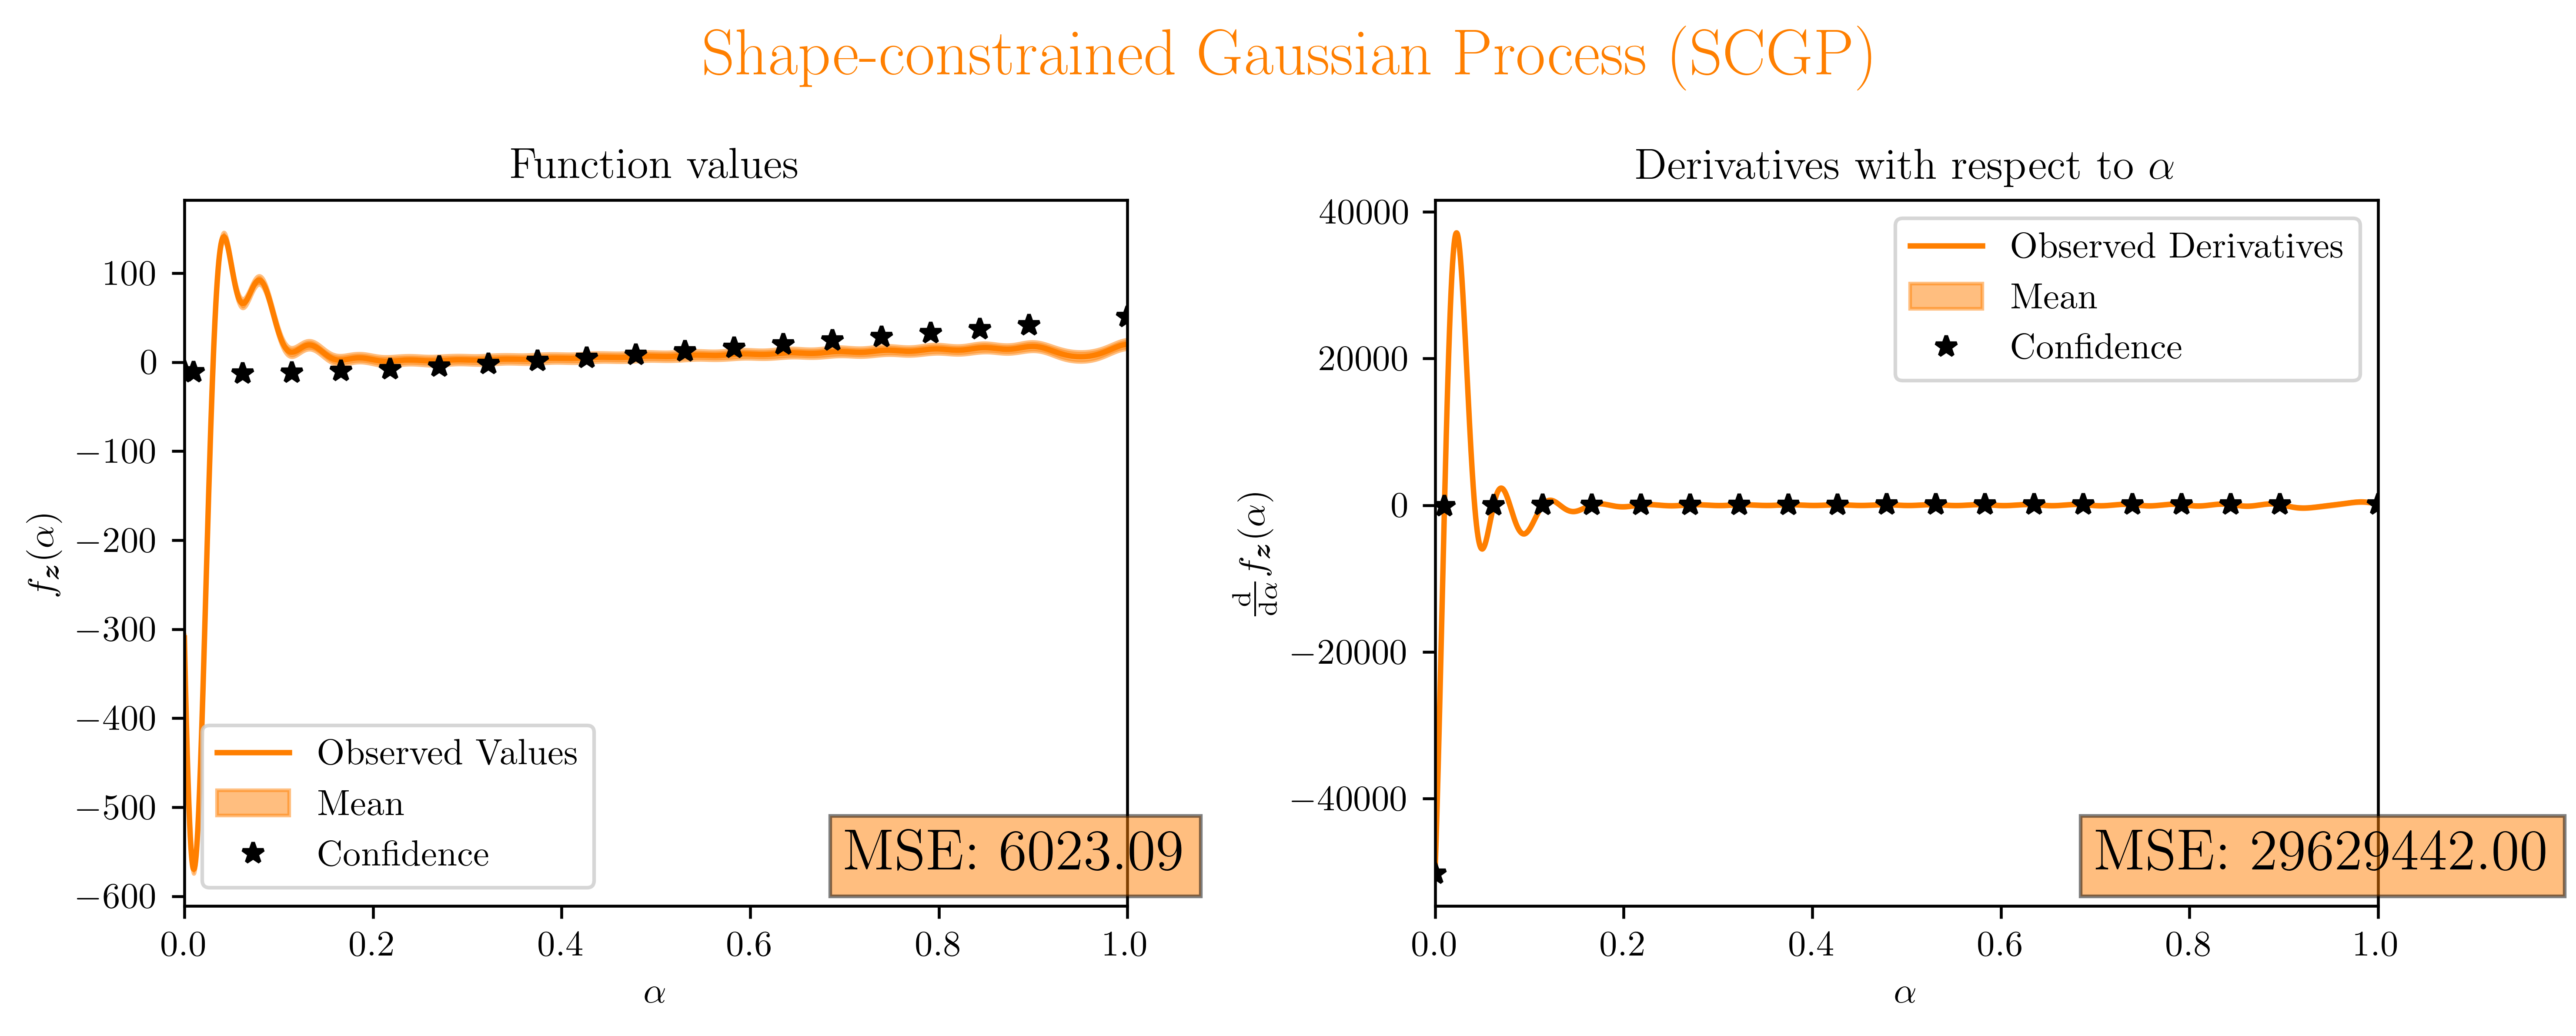
\includegraphics[width=.66\textwidth]{../experiments/uniform_new_HC/SCGP_20_nobs.png}
    \caption{ {\small Comparison between Gaussian Process with and without shape constraints under high curvature and regular grid evaluation. Source: author.}}
    \label{fig:uniformHC}
\end{figure}

In \zcref{fig:adaptiveHC}, both models perform poorly in the adaptive grid scenario with high curvature. In the case of the SCGP, the unsatisfactory fitting of the derivative process is a possible explanation for the model not performing as well as in previous scenarios.

\begin{figure}[H]
    \centering
    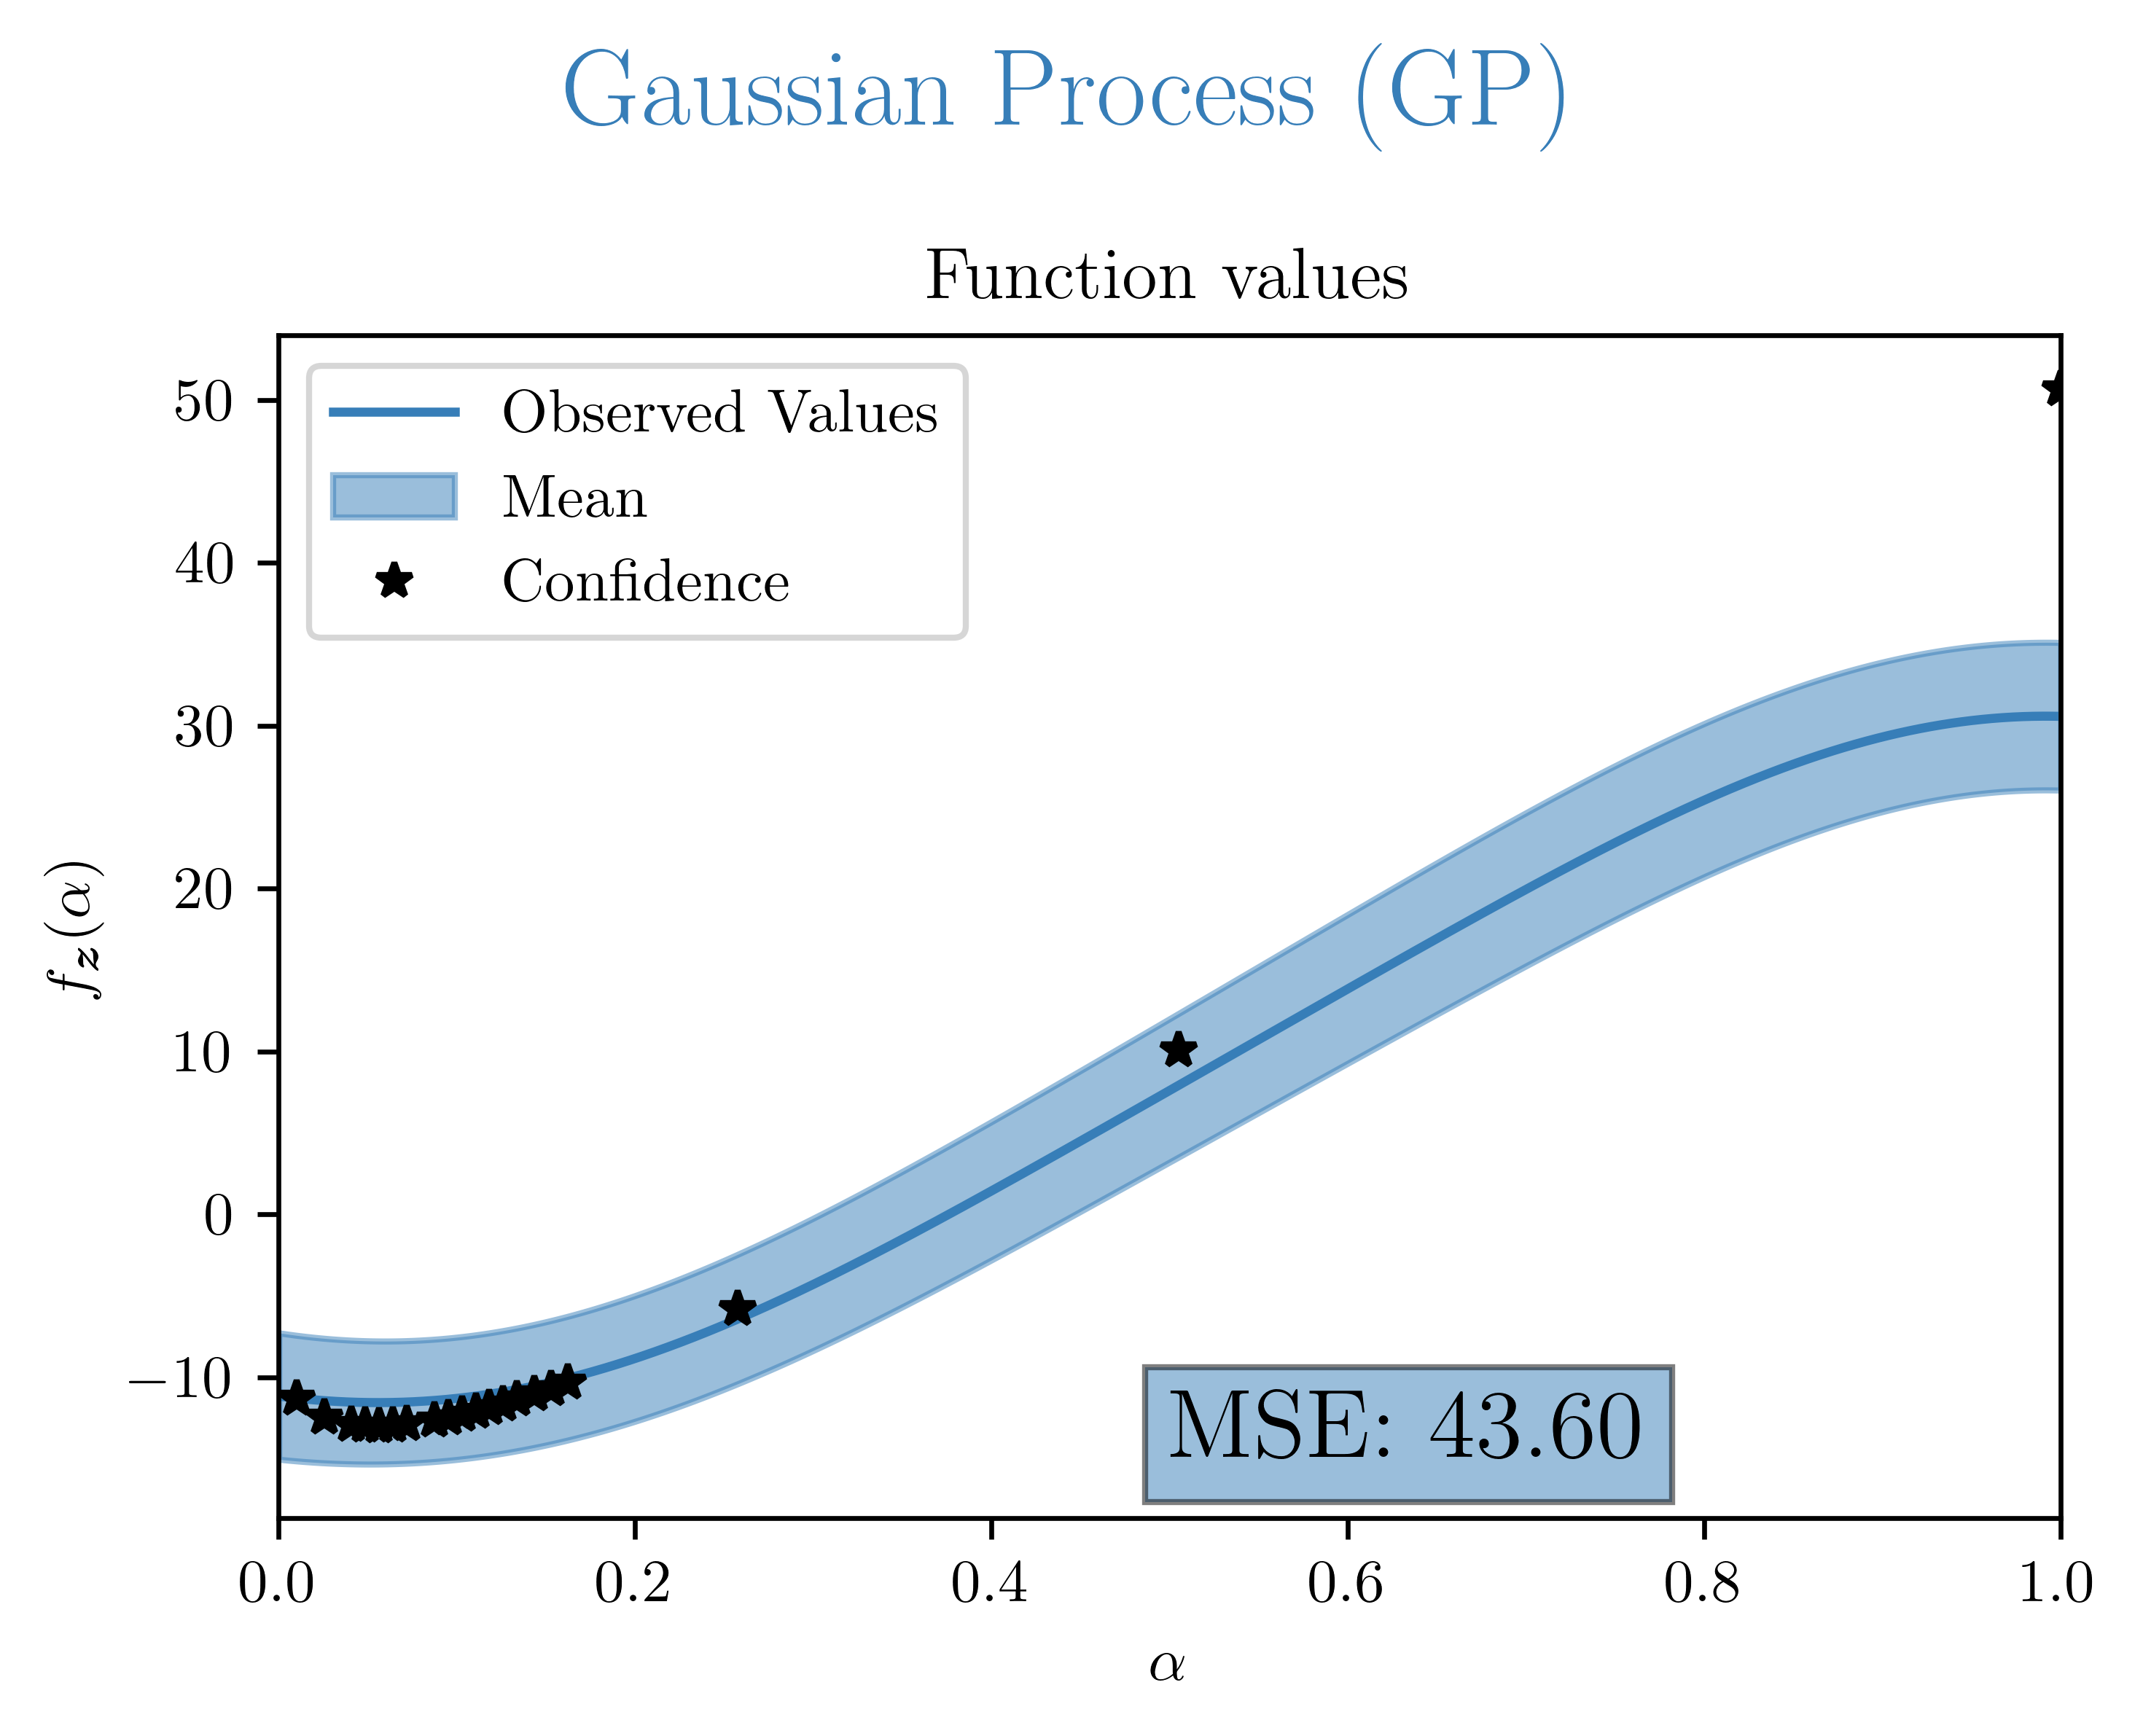
\includegraphics[width=.33\textwidth]{../experiments/adaptive_new_HC/GP_20_nobs.png}
    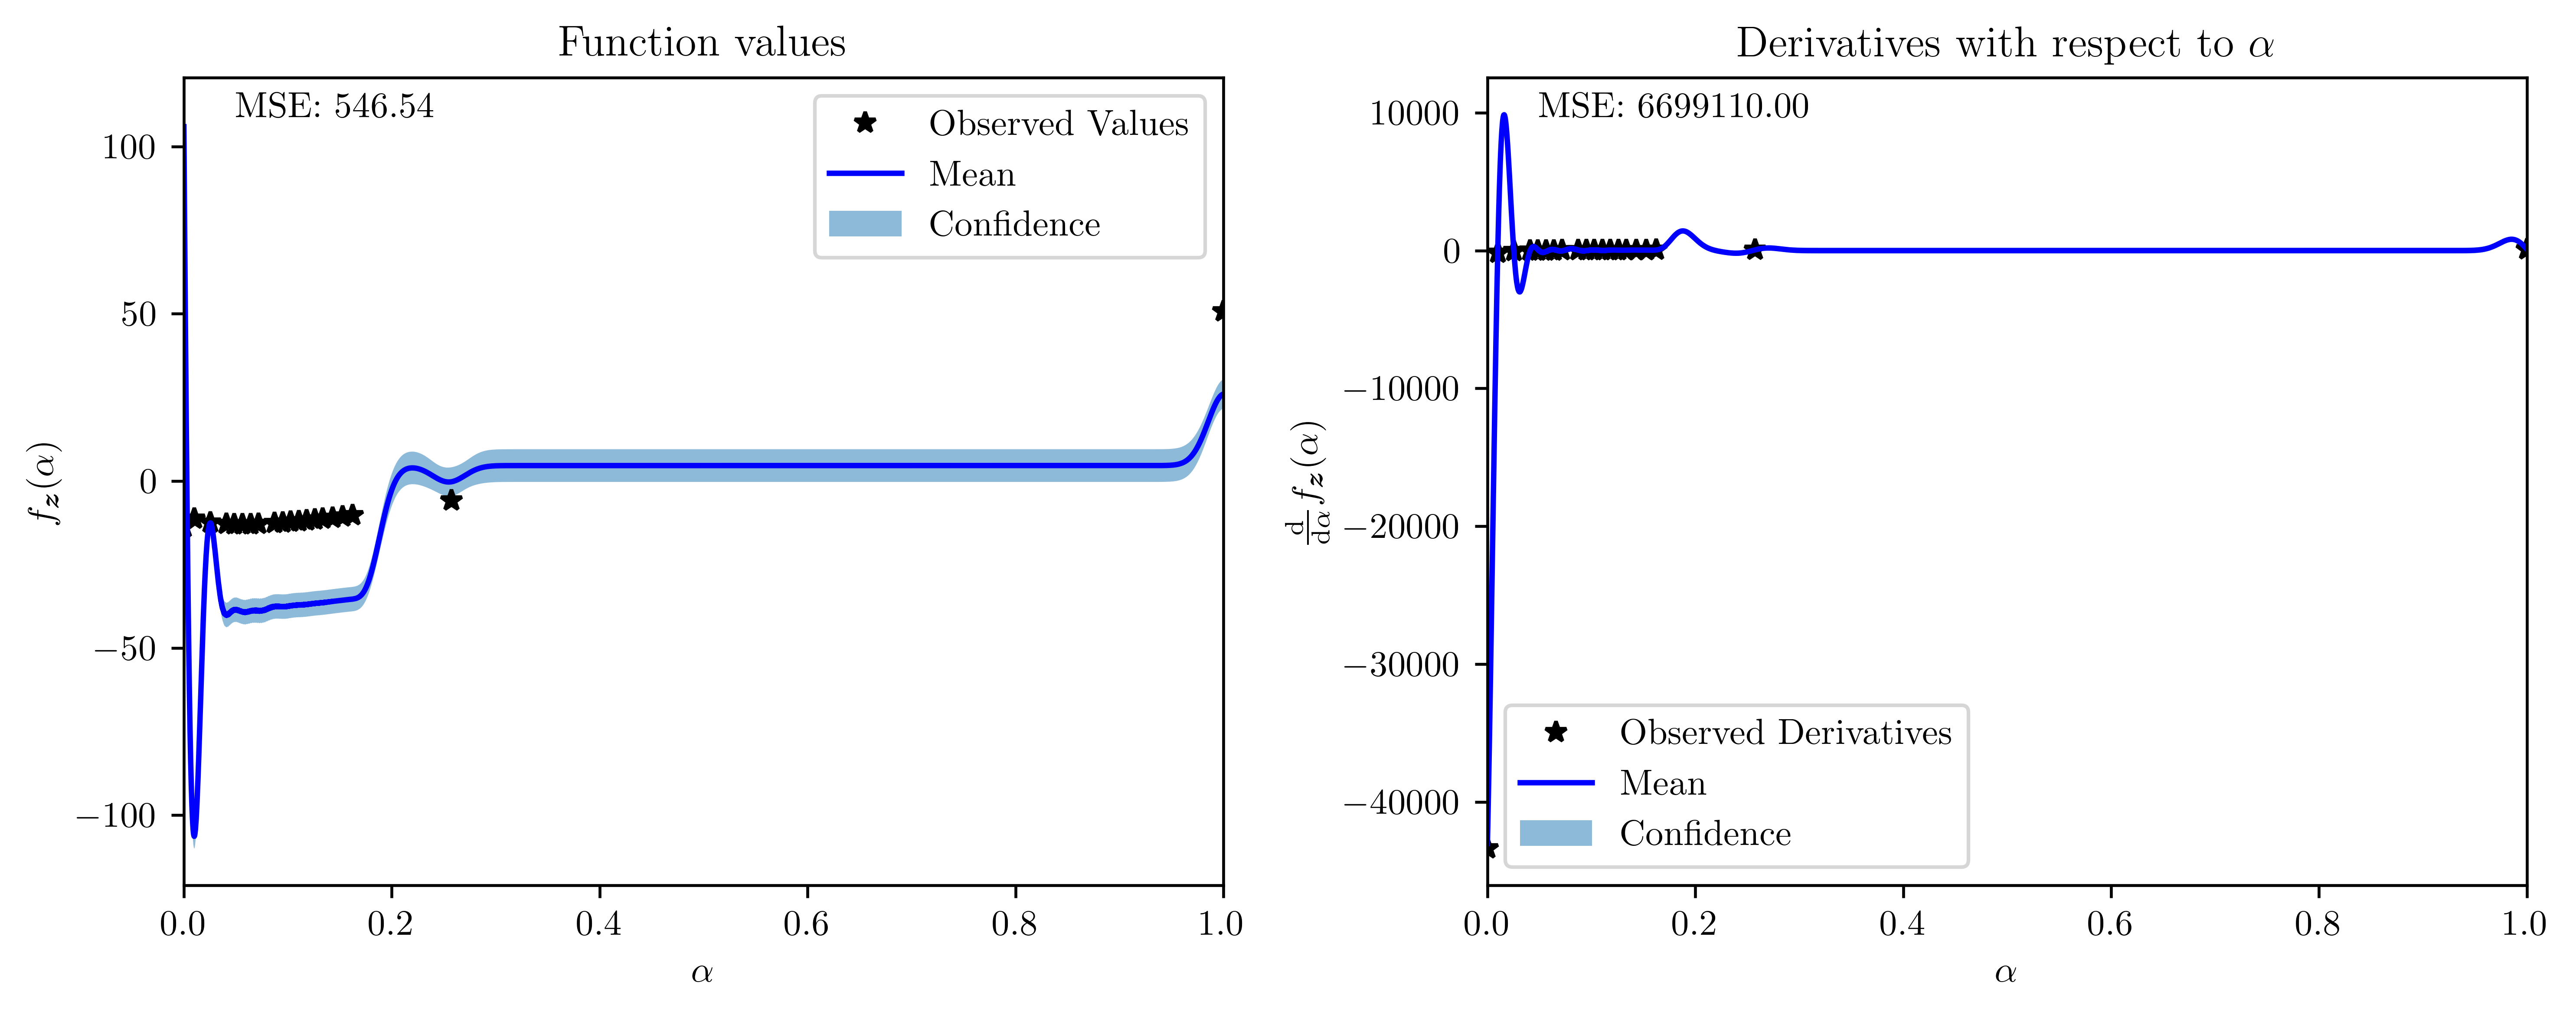
\includegraphics[width=.66\textwidth]{../experiments/adaptive_new_HC/SCGP_20_nobs.png}
    \caption{ {\small Comparison between Gaussian Process with and without shape constraints under high curvature and irregular grid evaluation. Source: author.}}
    \label{fig:adaptiveHC}
\end{figure}

\subsubsection{Reducing the Number of Observed Points}
\label{sec:reducingMC}

The second experiment consists of evaluating the fitting ability of the proposed methods under variations in the number of observed points.
For this, we will perform the fitting under medium curvature evaluated on a regular grid (which proved to be the best scenario in \zcref{sec:curvature}), but with \( M=\{6, 8, 10, 12, 14, 16, 18\} \) evaluations of \( f_{\bfz}(\alpha) \).

Observing \zcref{fig:reducingMCpt1}, it is possible to see that the traditional Gaussian Process is outperformed starting from 8 observed points, with an MSE approximately 18 times higher than the SCGP. Furthermore, in \zcref{fig:reducingMCpt2}, we see that the SCGP is able to fit the derivative process satisfactorily from 12 observed points, outperforming the traditional Gaussian Process in all scenarios.

\begin{figure}[H]
    \centering
    \resizebox{\textwidth}{!}{
    \begin{tabular}{|c|c|}
        \hline
        \subf{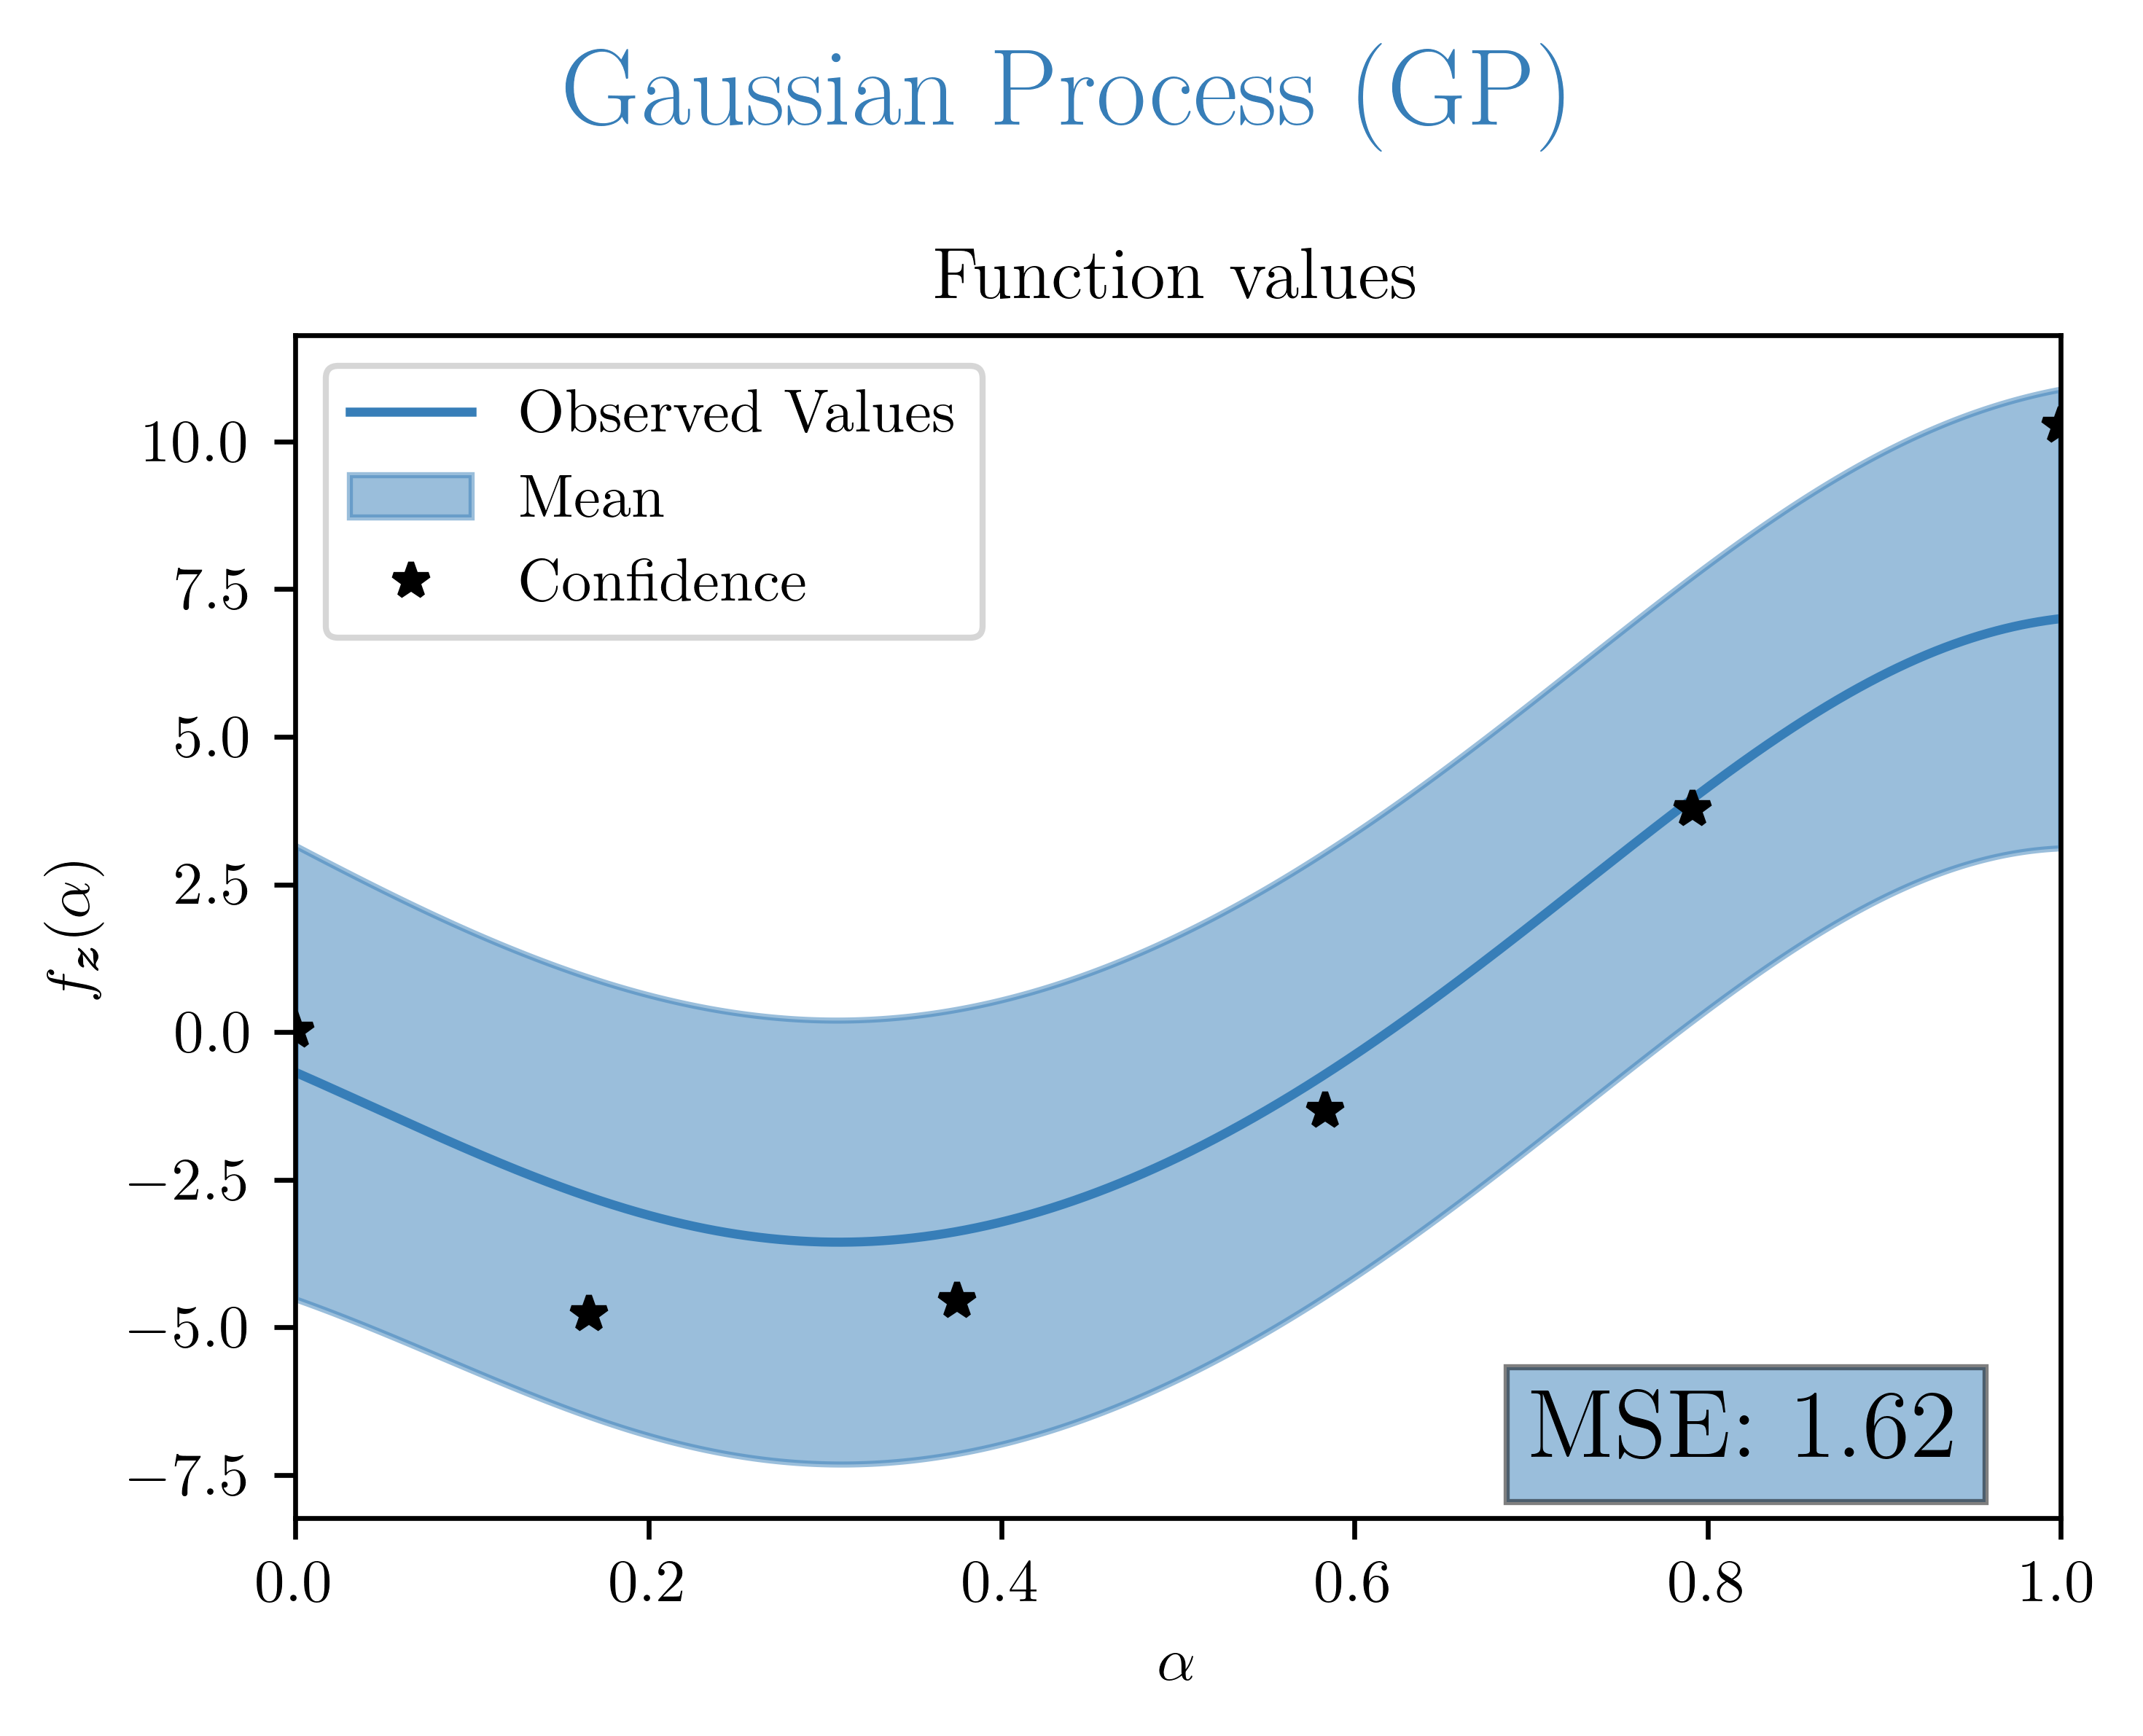
\includegraphics[width=.33\textwidth]{../experiments/uniform_new_MC/GP_6_nobs.png}}{GP with 6 evaluations} & \subf{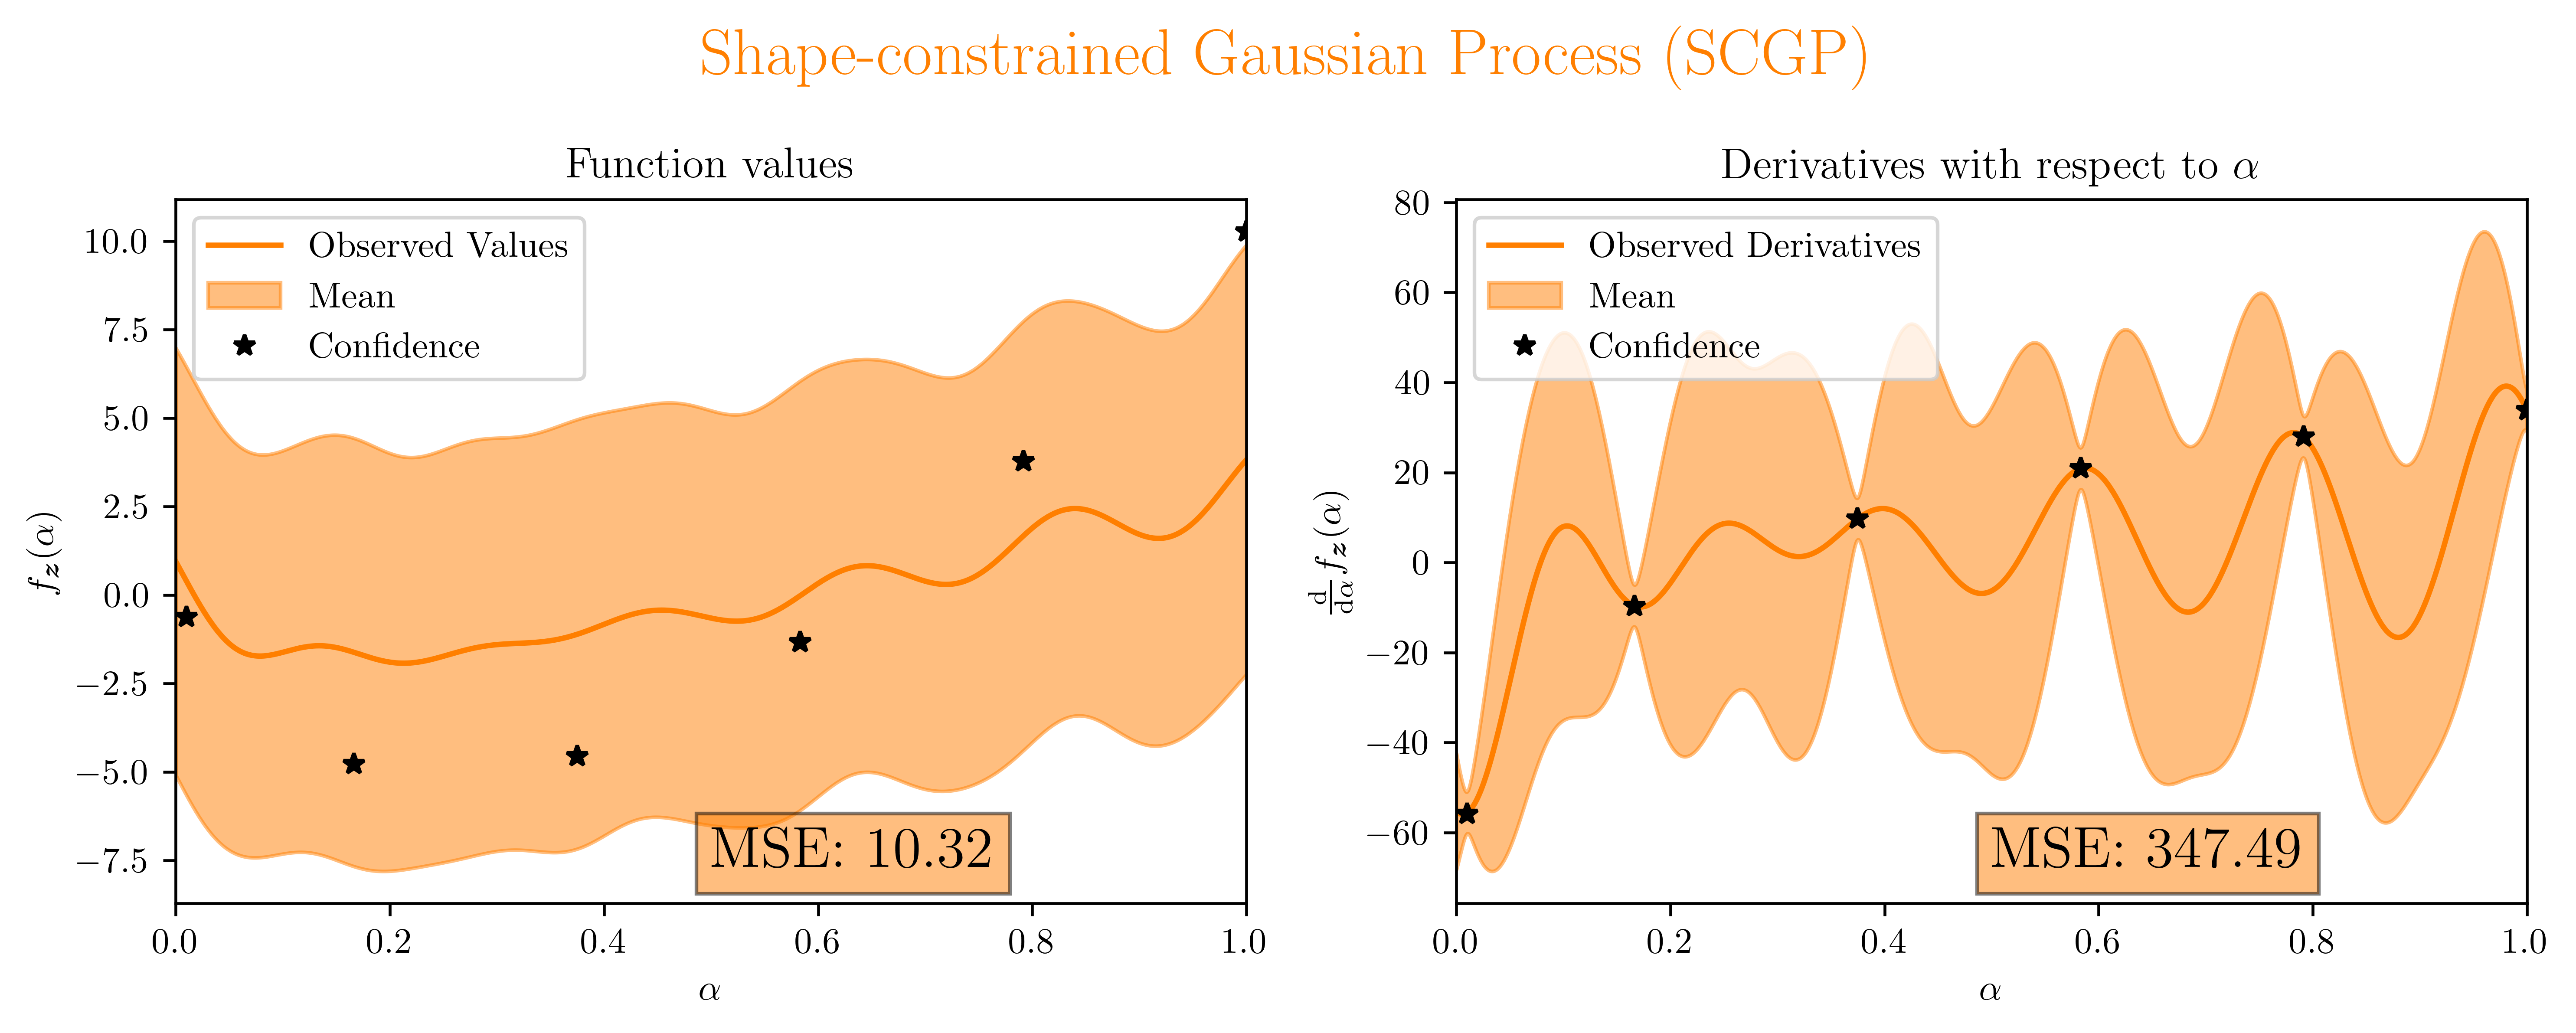
\includegraphics[width=.66\textwidth]{../experiments/uniform_new_MC/SCGP_6_nobs.png}}{SCGP with 6 evaluations} \\
        \hline
        \subf{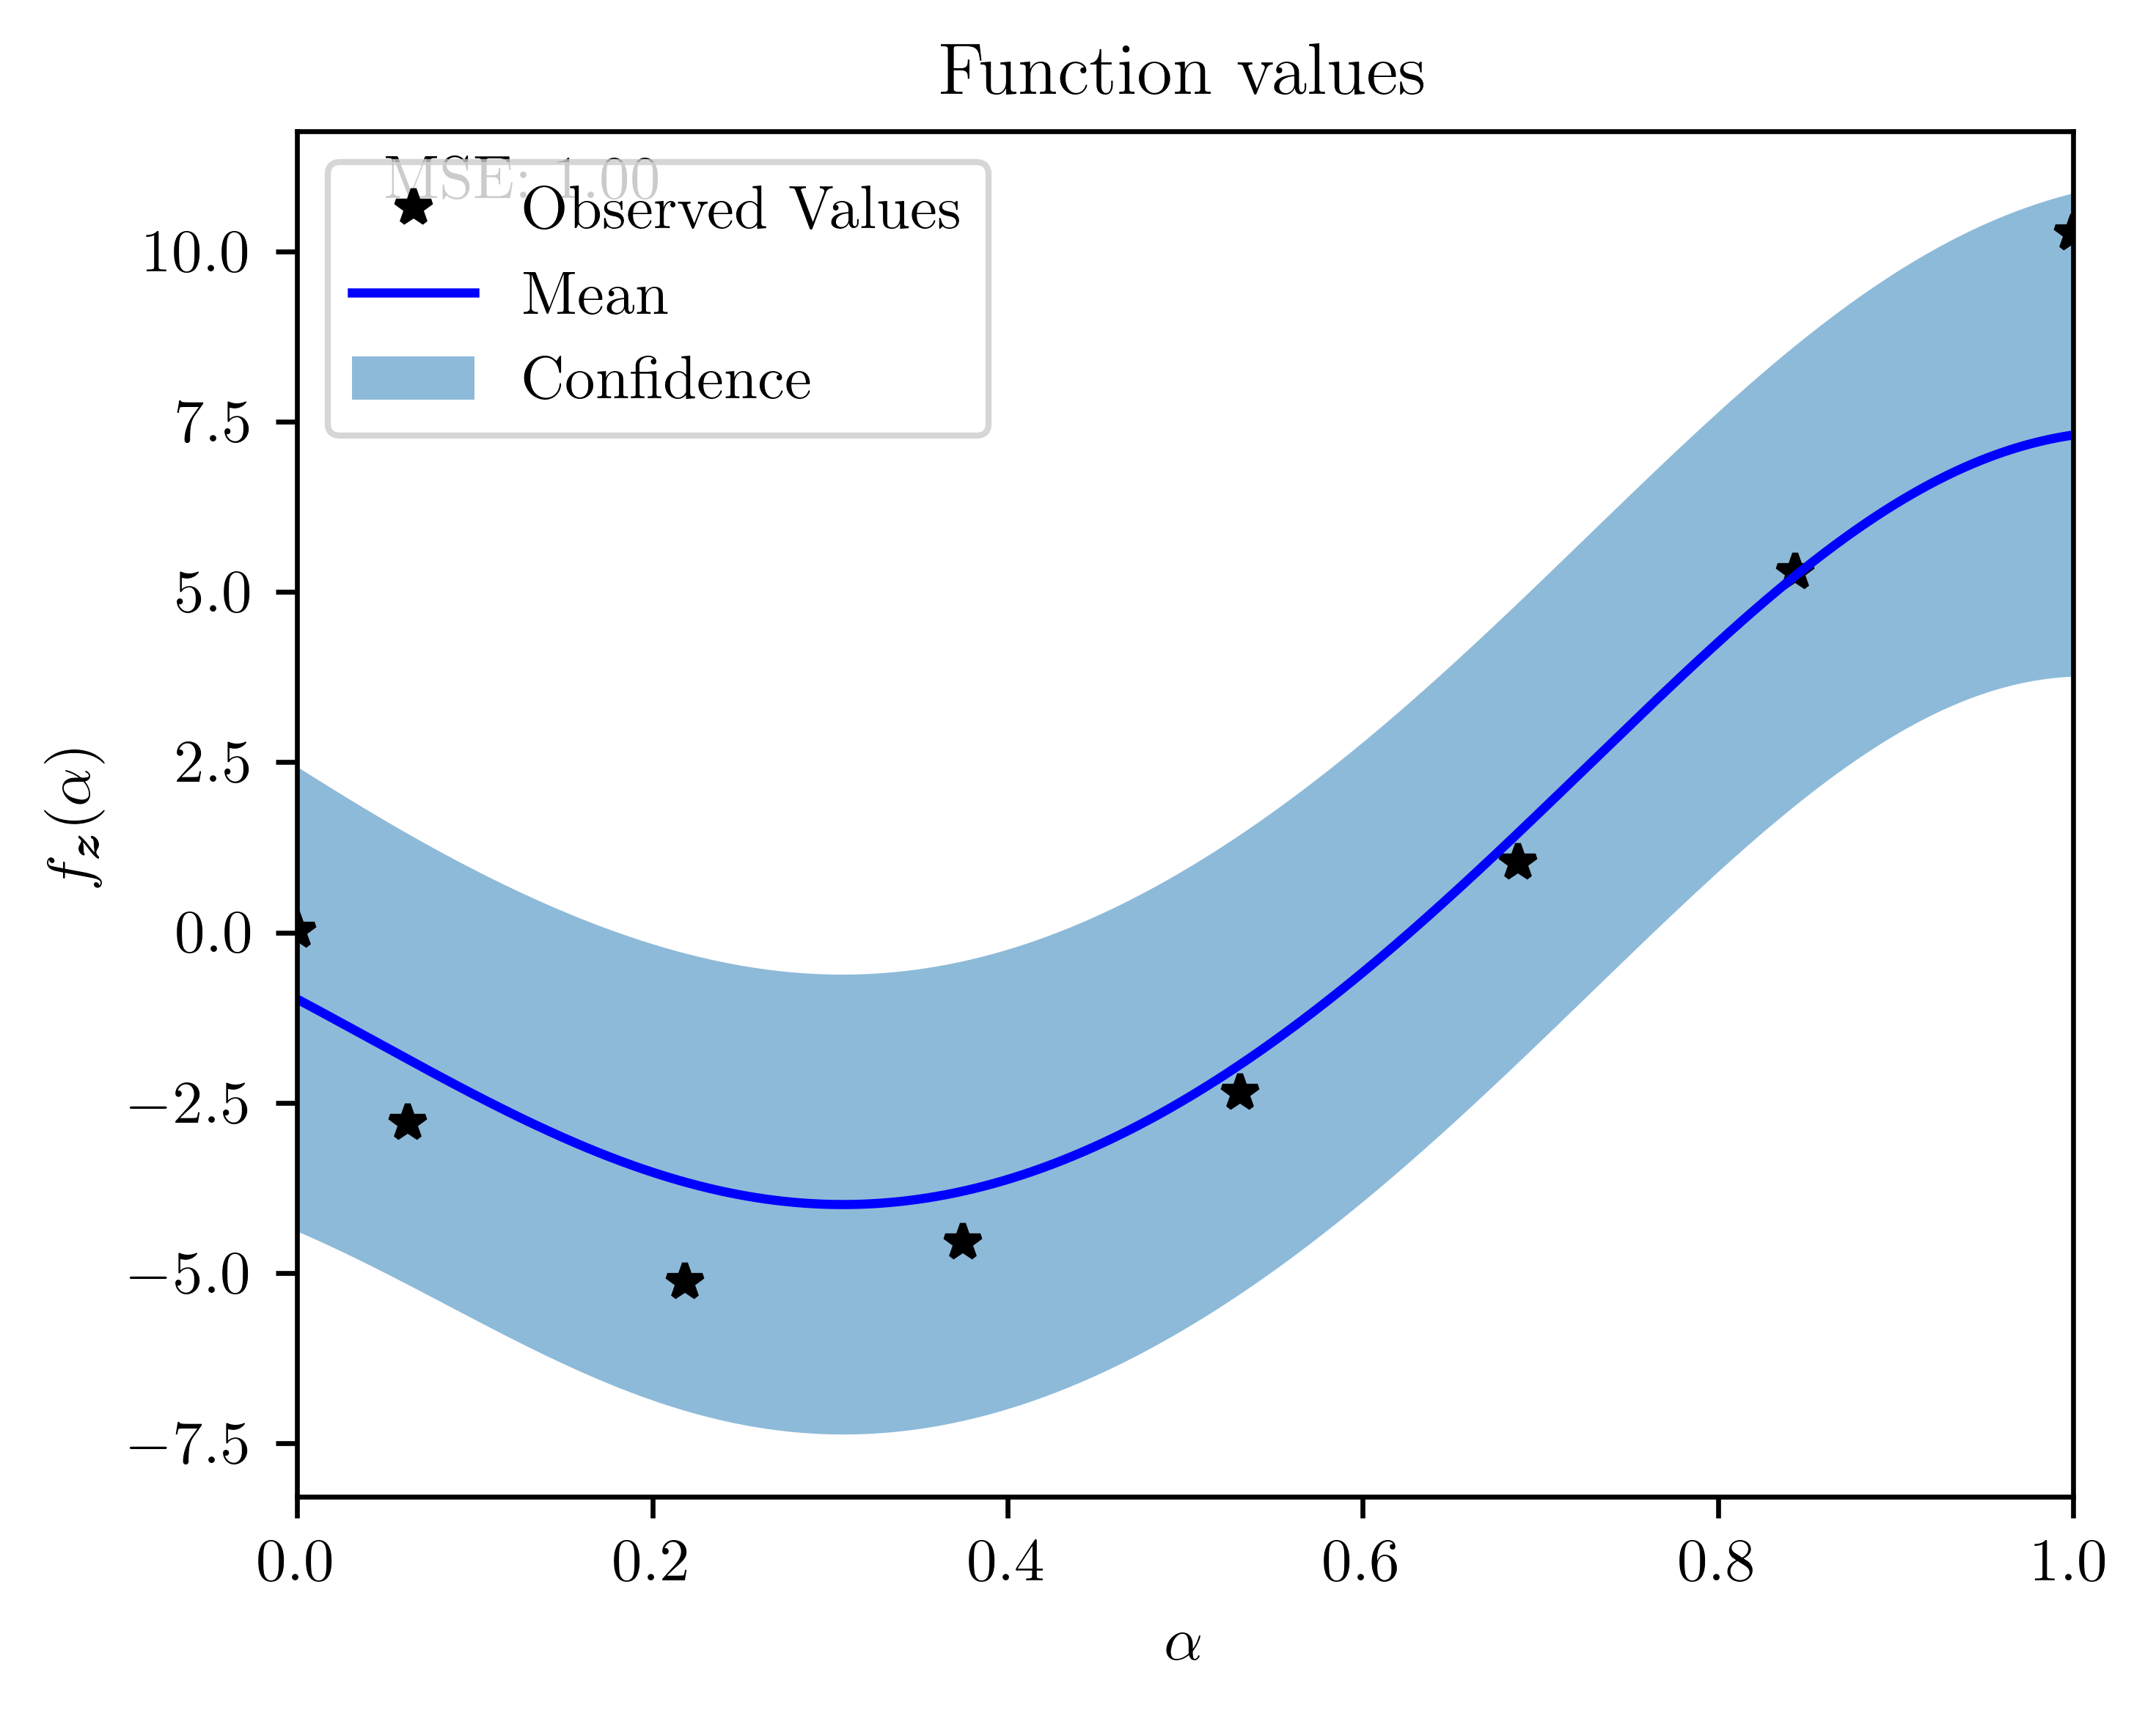
\includegraphics[width=.33\textwidth]{../experiments/uniform_new_MC/GP_8_nobs.png}}{GP with 8 evaluations} & \subf{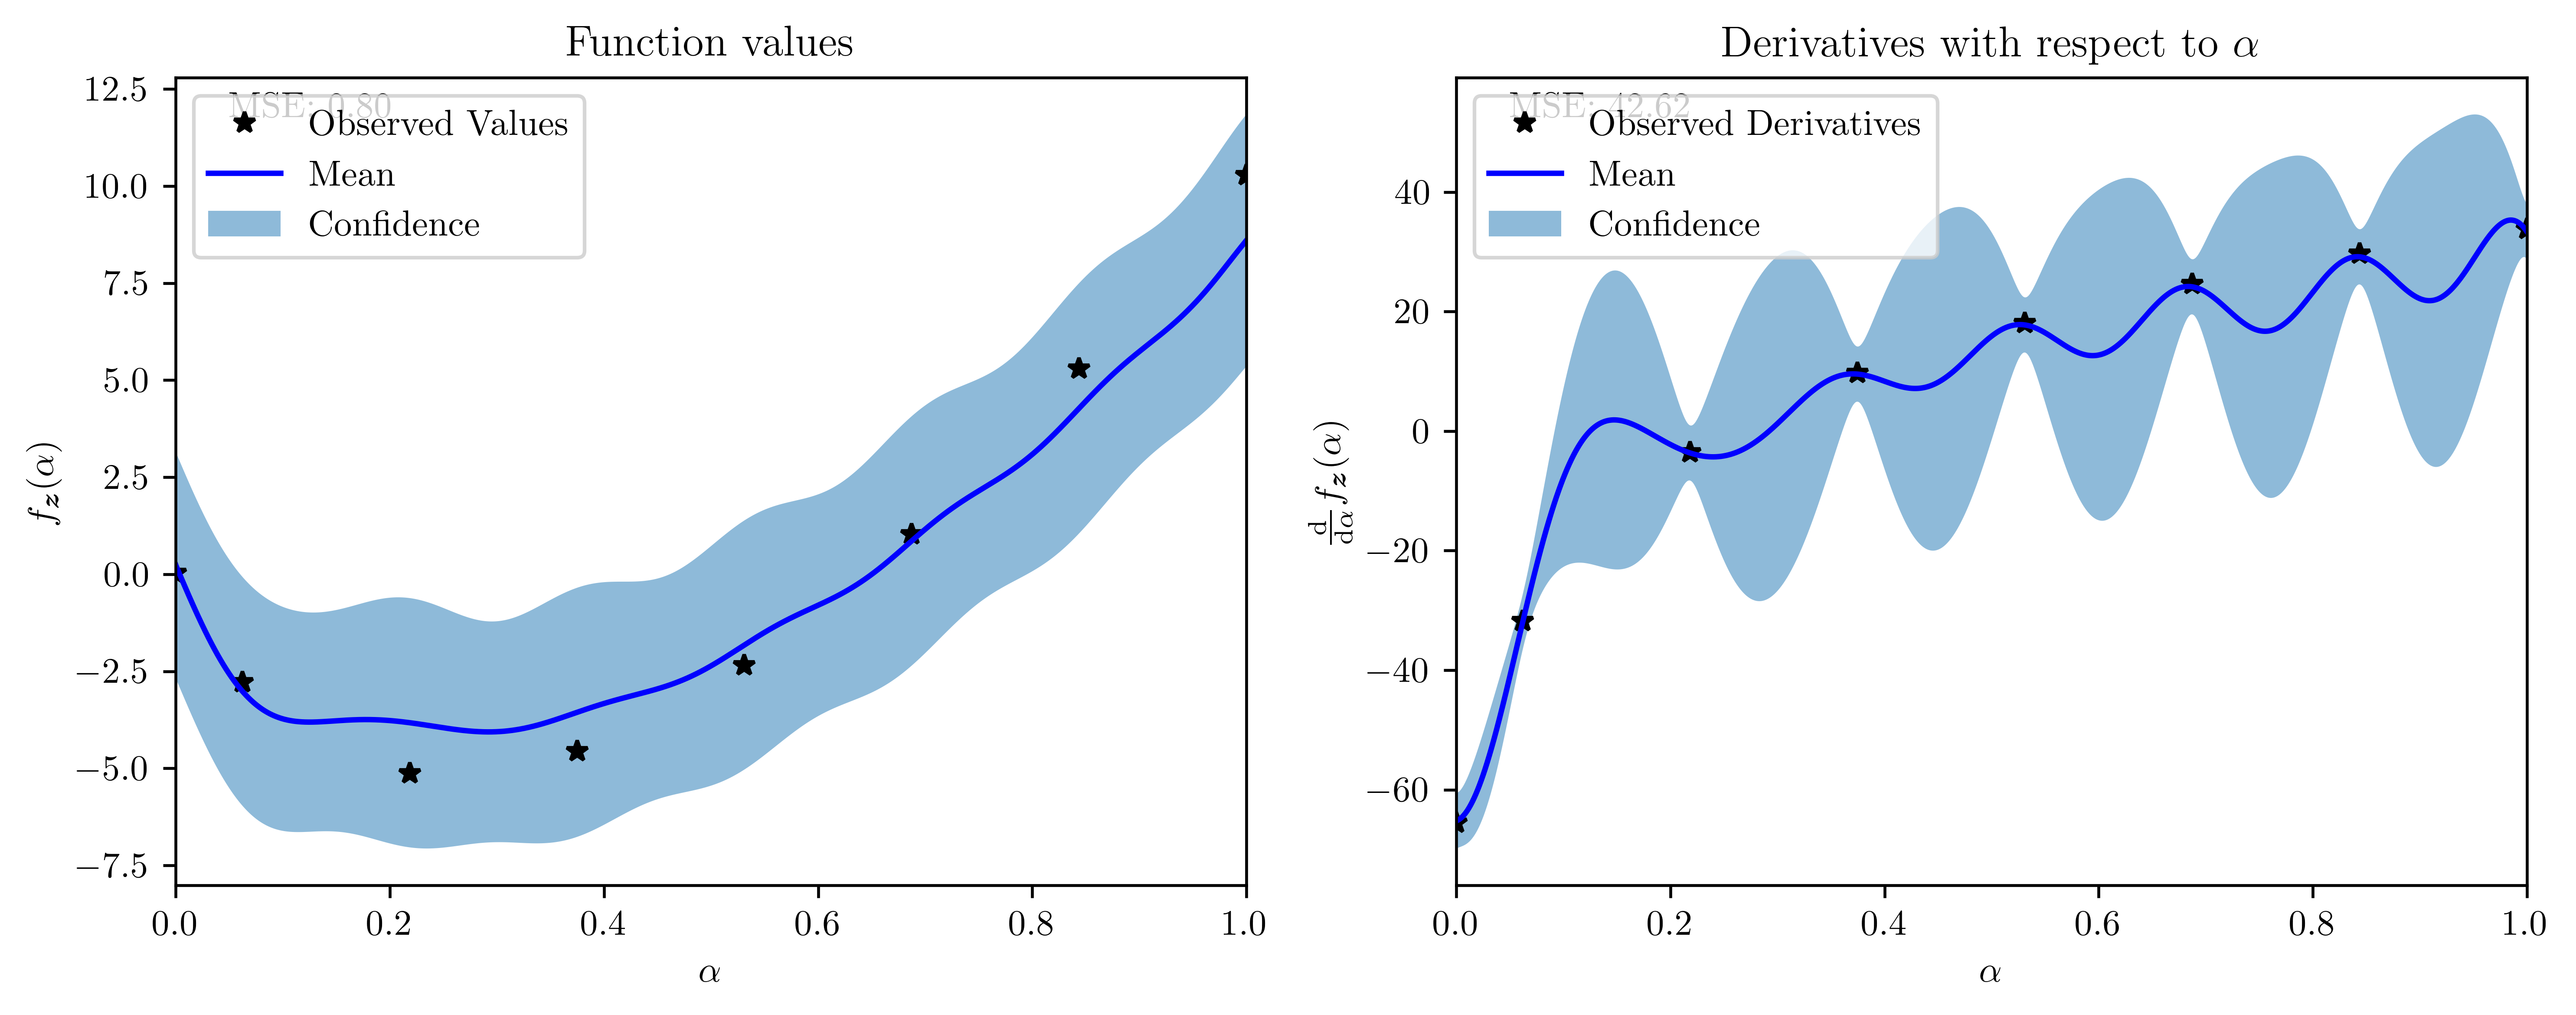
\includegraphics[width=.66\textwidth]{../experiments/uniform_new_MC/SCGP_8_nobs.png}}{SCGP with 8 evaluations} \\
        \hline
        \subf{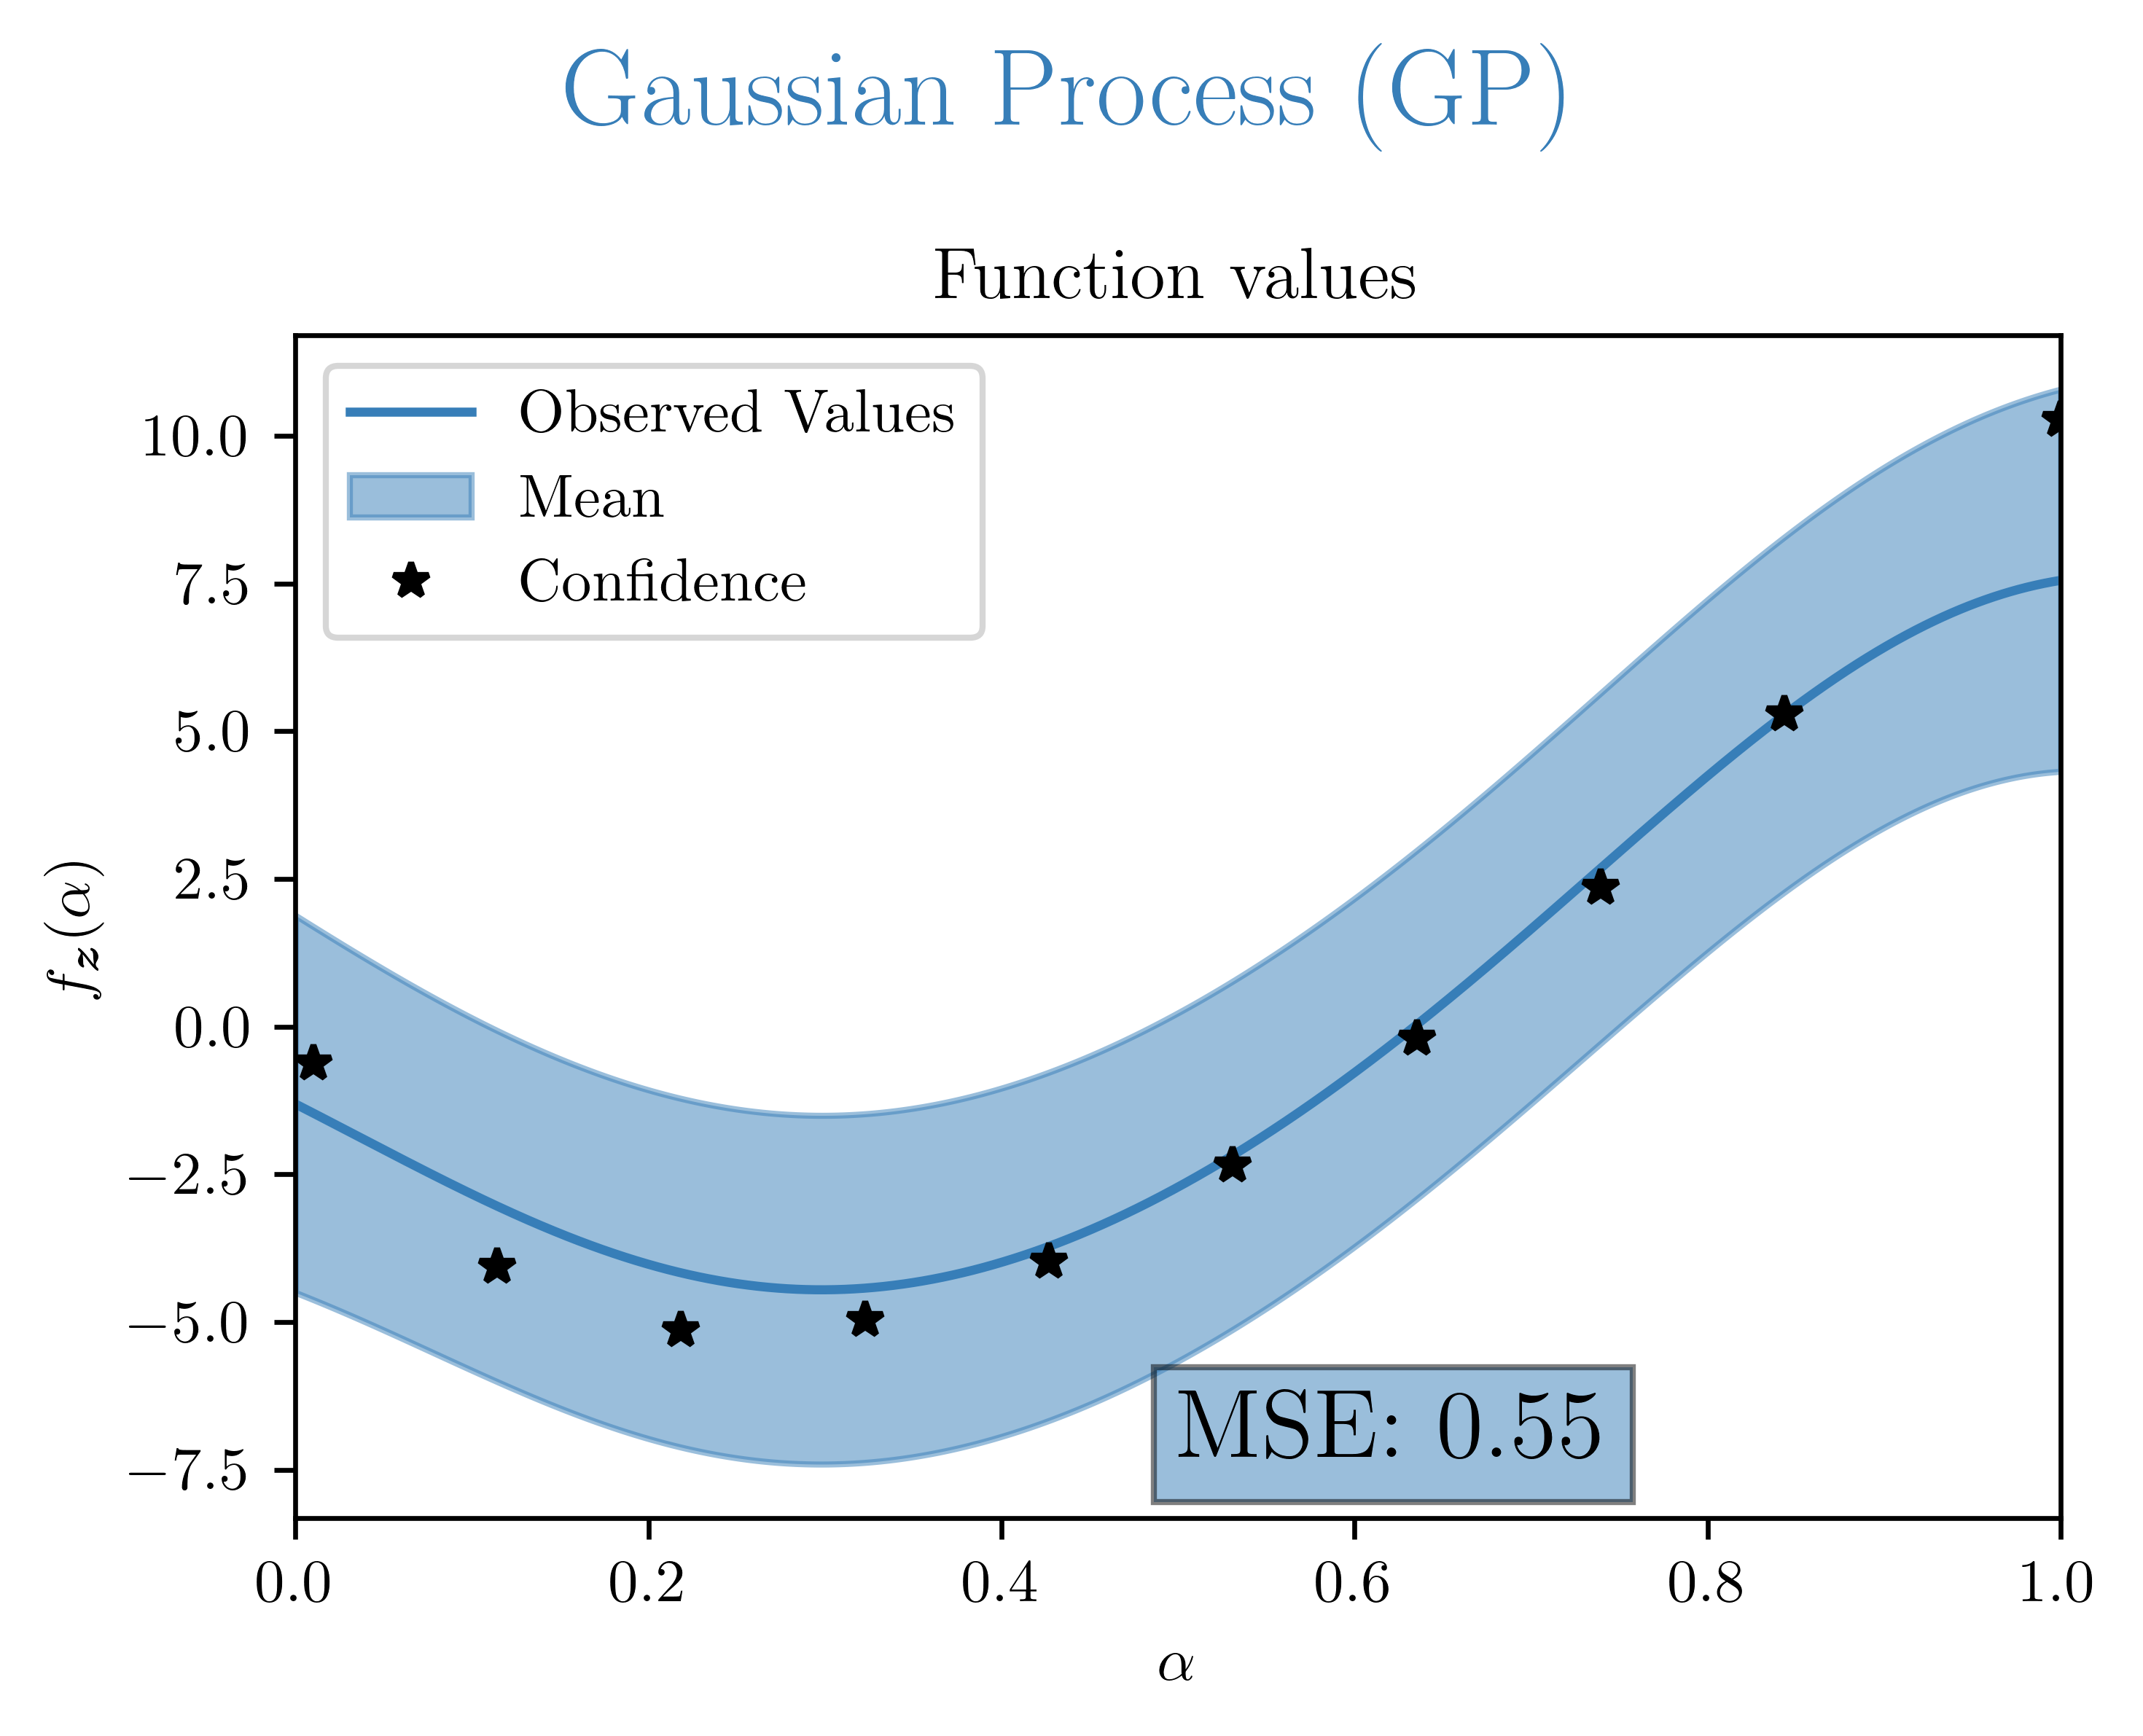
\includegraphics[width=.33\textwidth]{../experiments/uniform_new_MC/GP_10_nobs.png}}{GP with 10 evaluations} & \subf{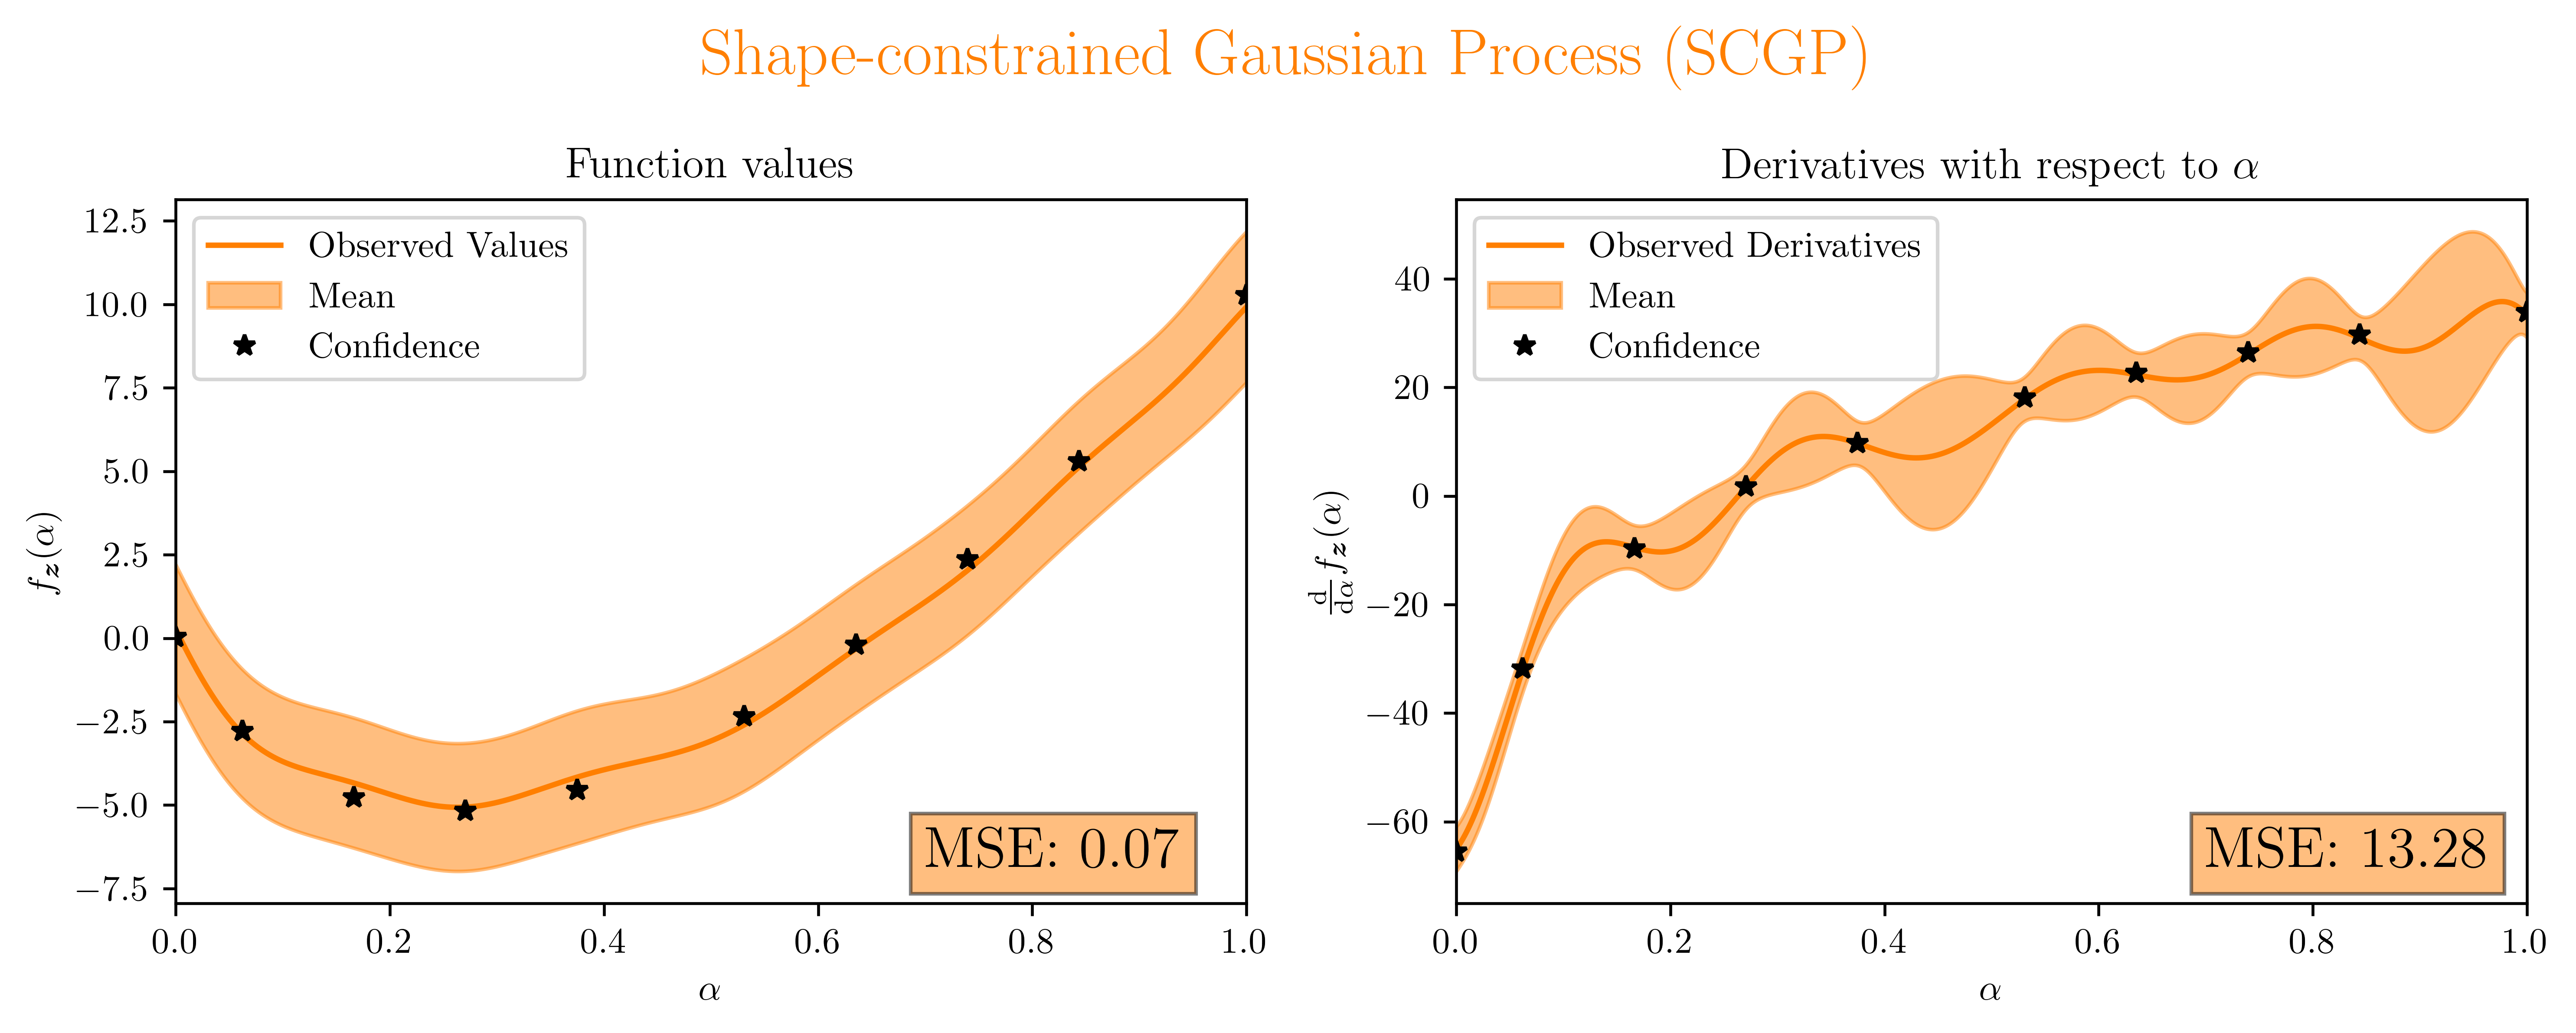
\includegraphics[width=.66\textwidth]{../experiments/uniform_new_MC/SCGP_10_nobs.png}}{SCGP with 10 evaluations} \\
        \hline
    \end{tabular}}
    \caption{ {\small Comparison between Gaussian Process with and without shape constraints under medium curvature and regular grid evaluation (6 to 10 points). Source: author.}}
    \label{fig:reducingMCpt1}
\end{figure}

\begin{figure}[H]
    \centering
    \resizebox{\textwidth}{!}{
    \begin{tabular}{|c|c|}
        \hline
        \subf{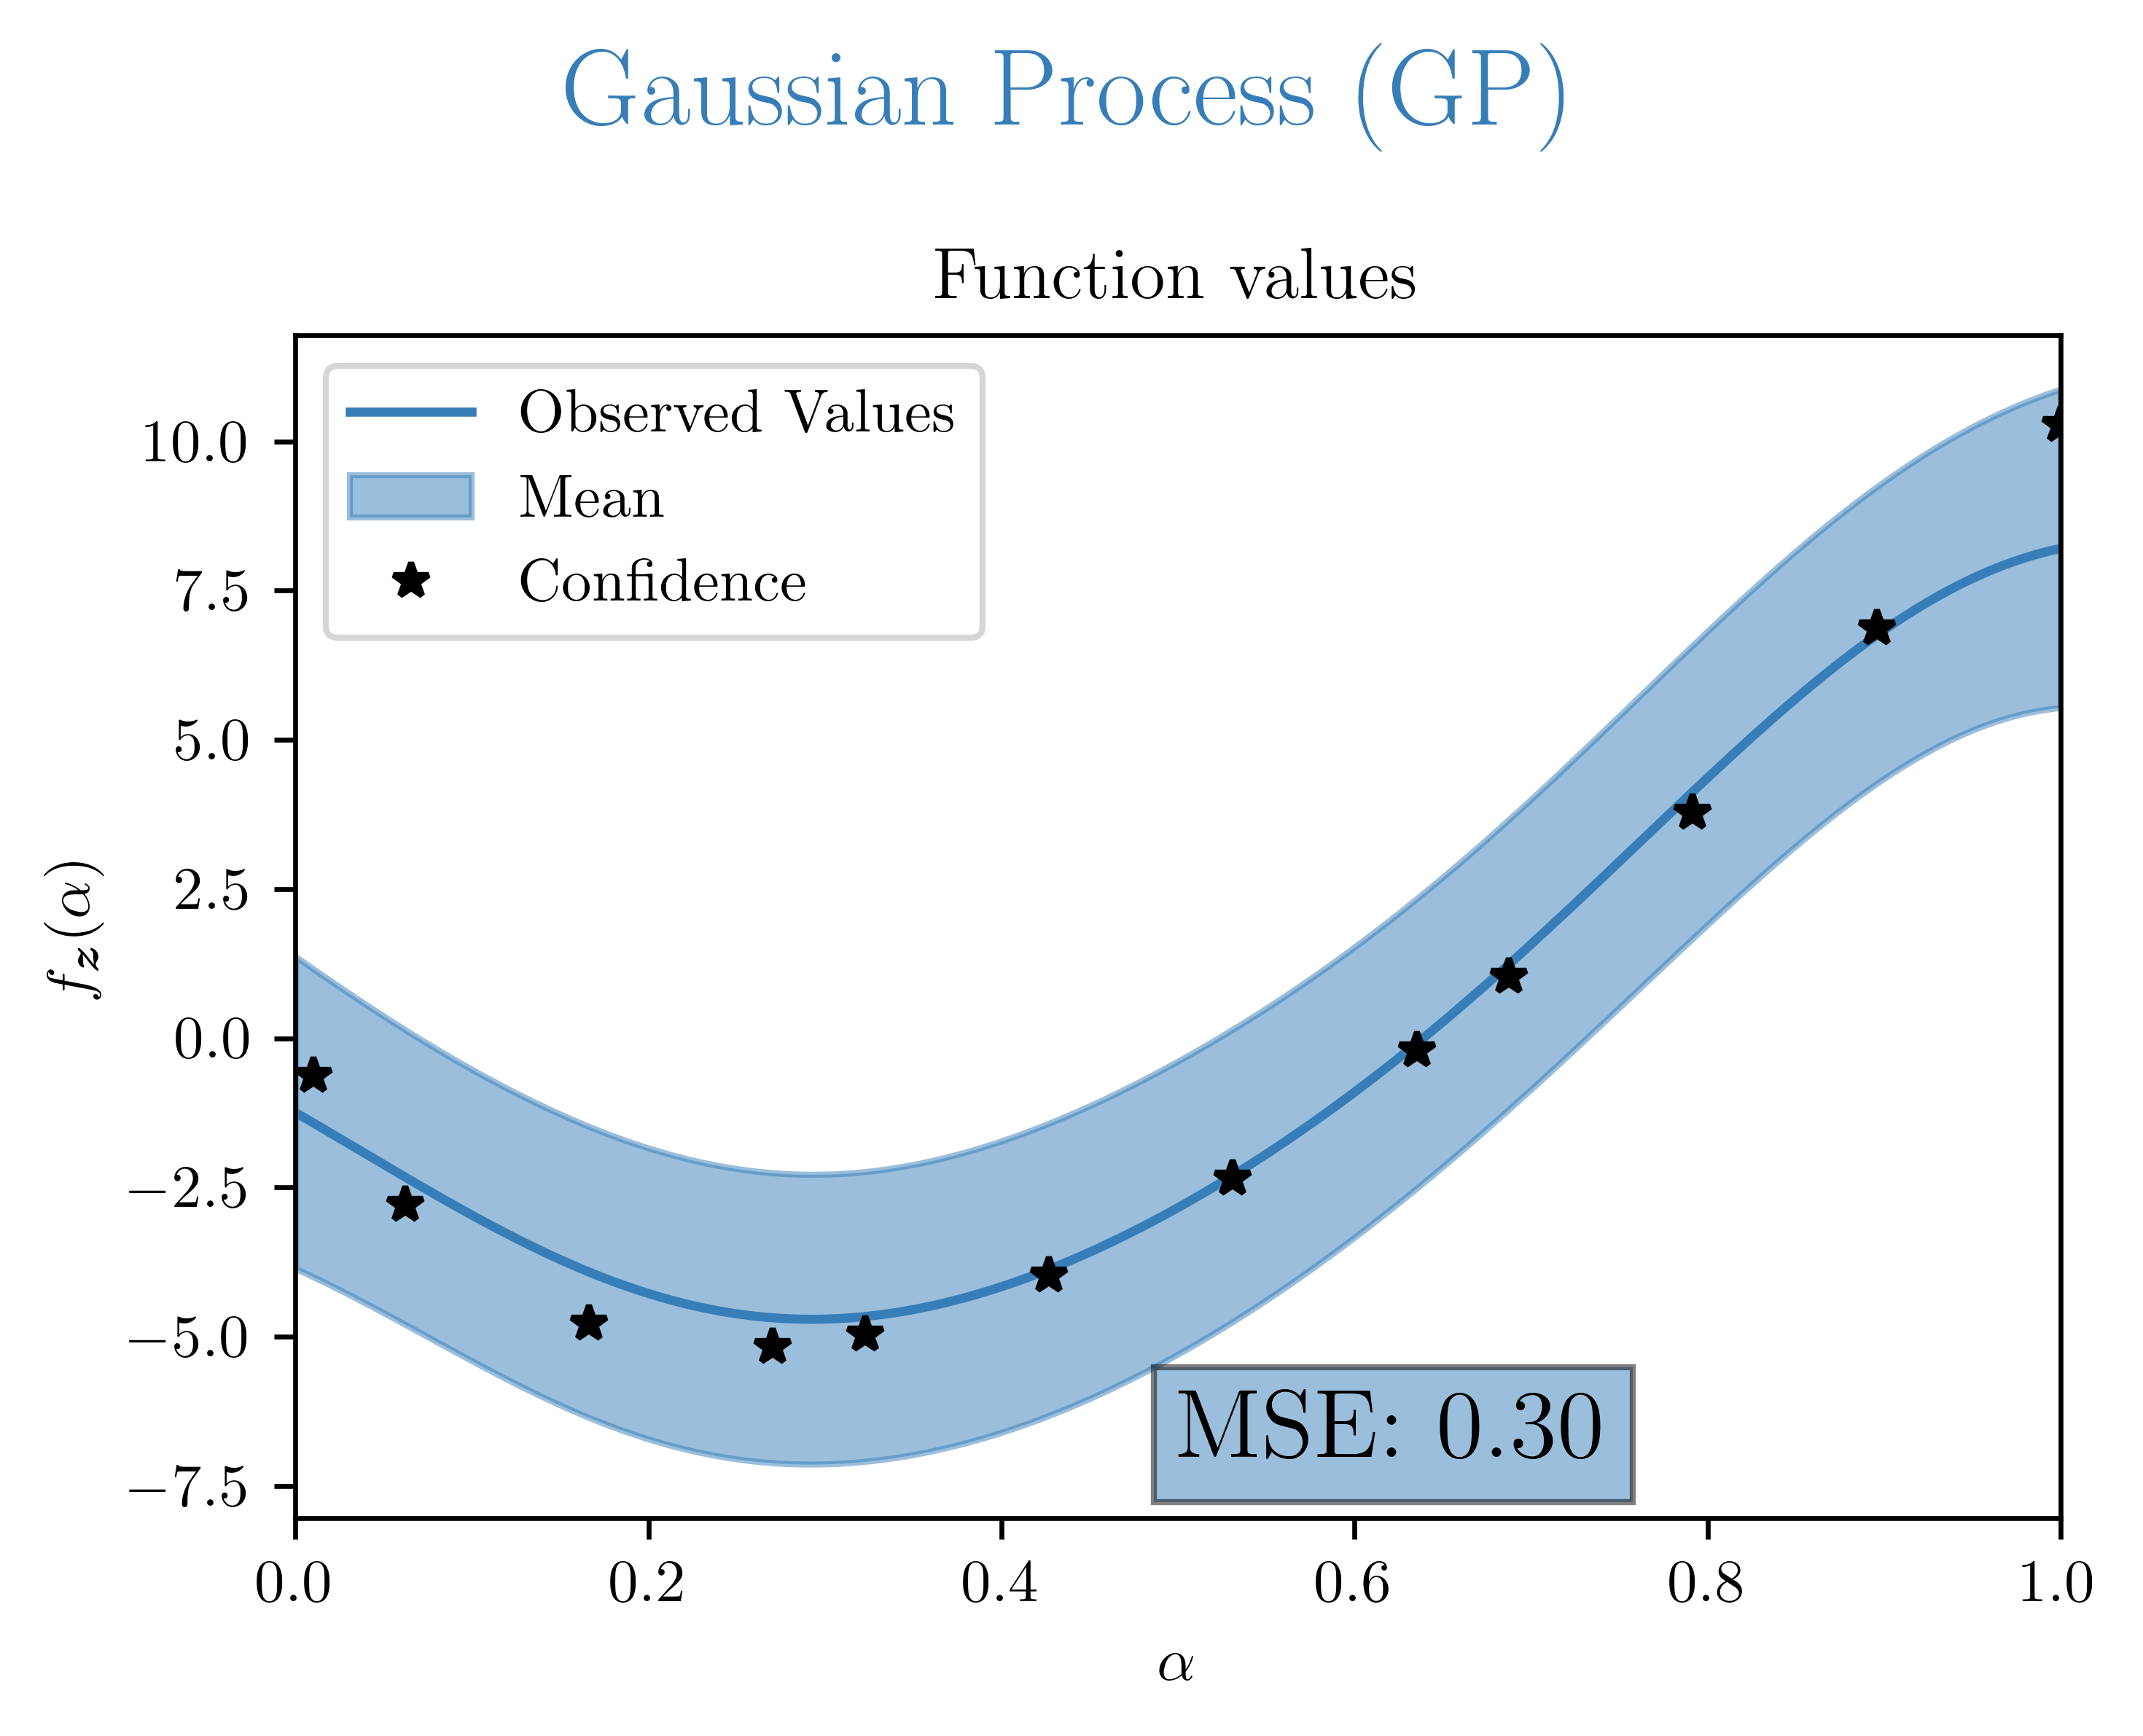
\includegraphics[width=.33\textwidth]{../experiments/uniform_new_MC/GP_12_nobs.png}}{GP with 12 evaluations} & \subf{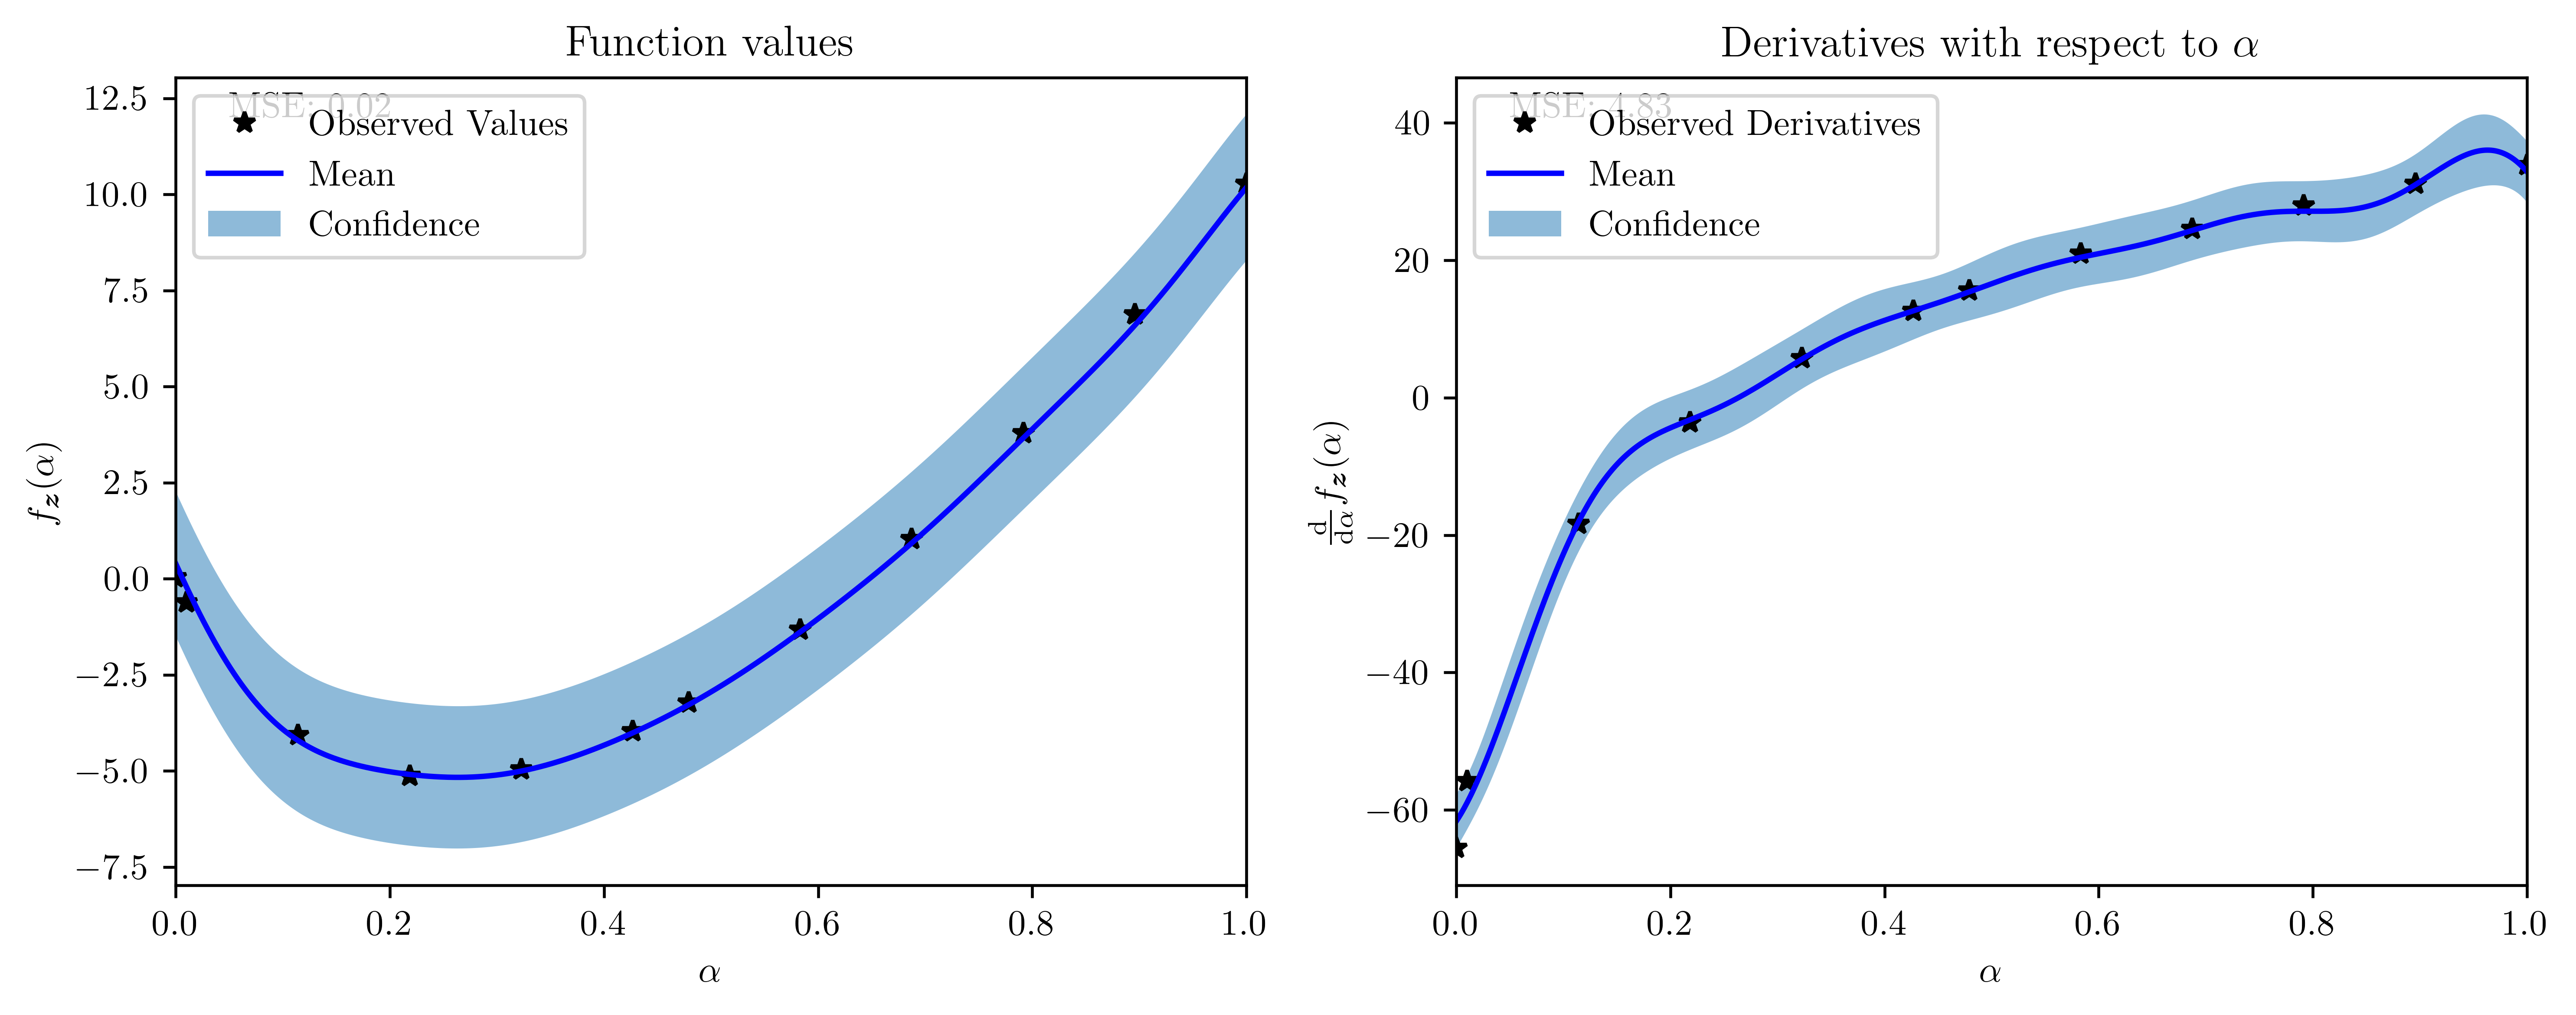
\includegraphics[width=.66\textwidth]{../experiments/uniform_new_MC/SCGP_12_nobs.png}}{SCGP with 12 evaluations} \\
        \hline
        \subf{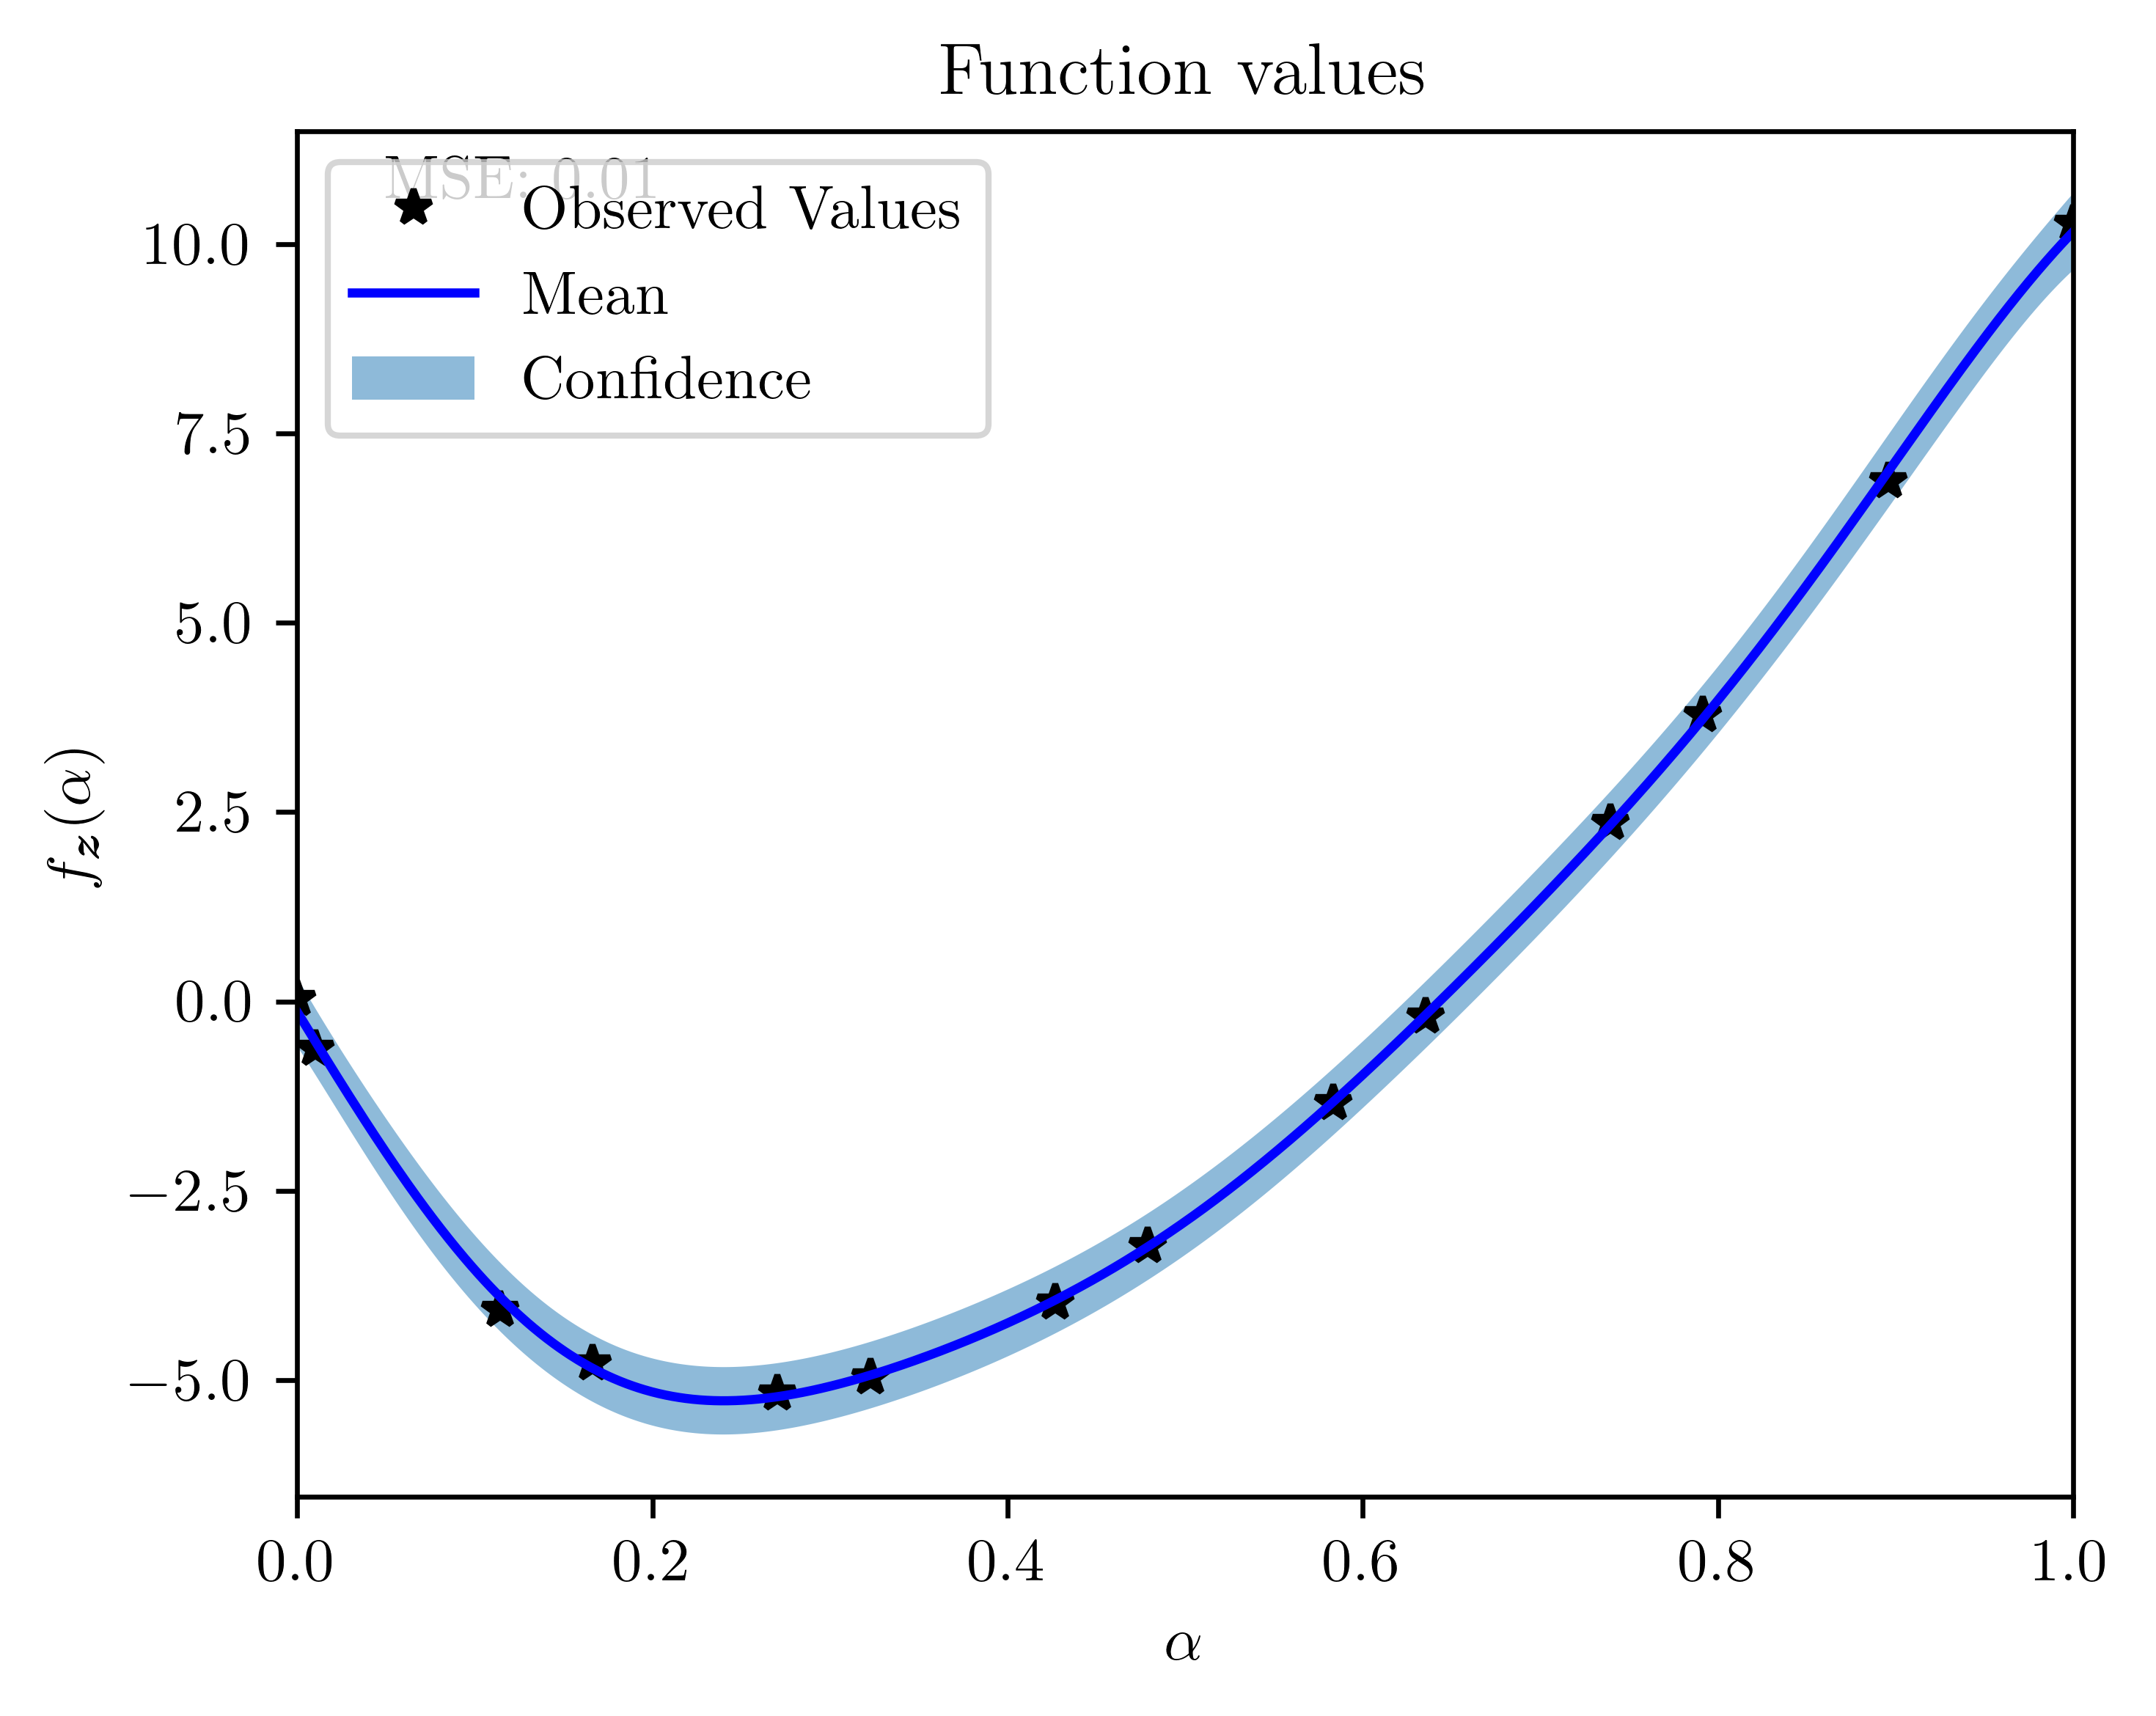
\includegraphics[width=.33\textwidth]{../experiments/uniform_new_MC/GP_14_nobs.png}}{GP with 14 evaluations} & \subf{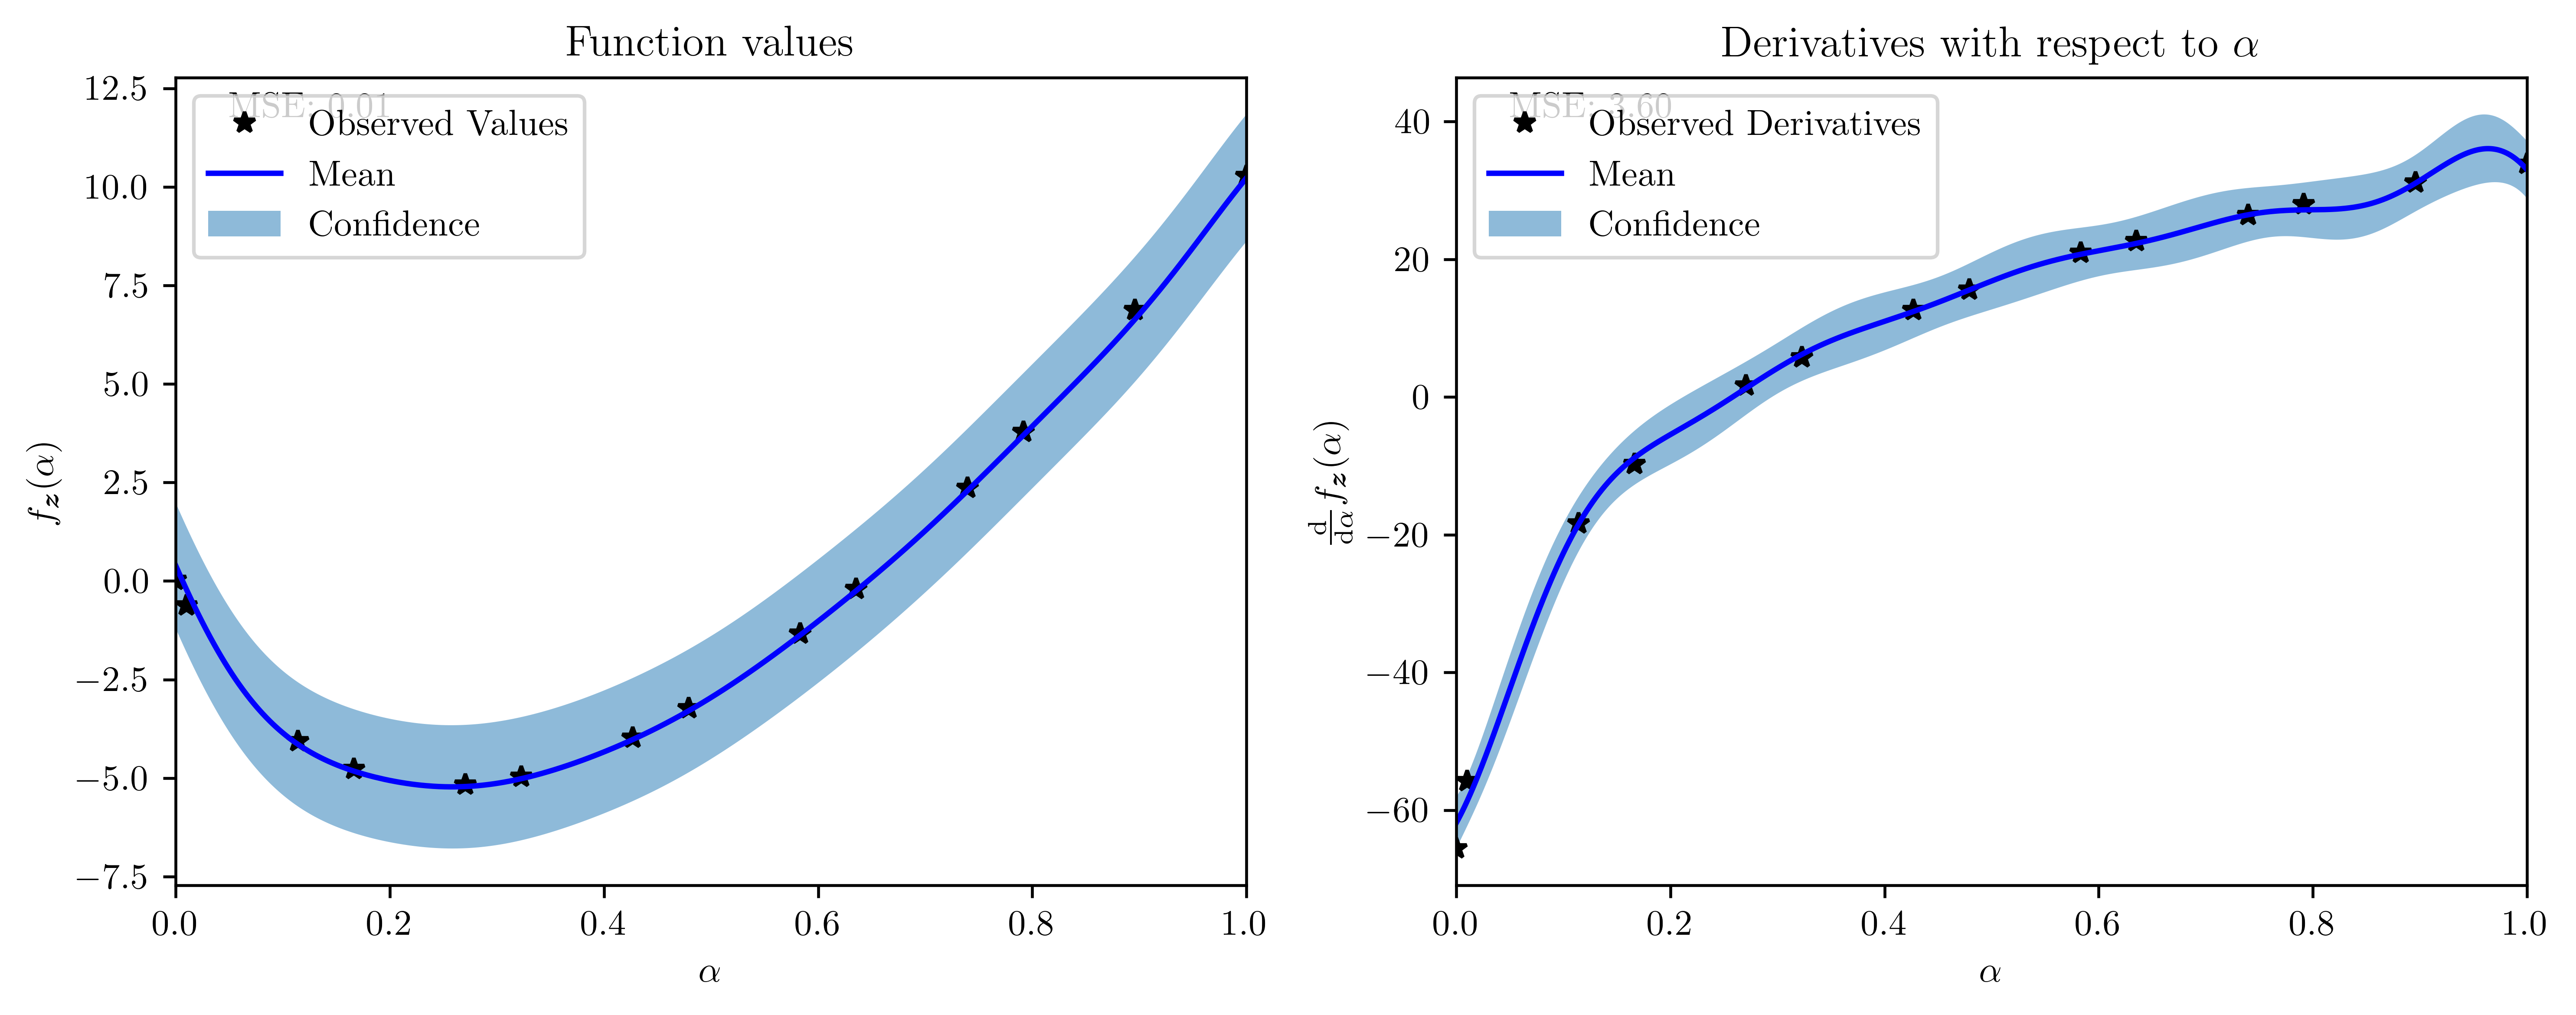
\includegraphics[width=.66\textwidth]{../experiments/uniform_new_MC/SCGP_14_nobs.png}}{SCGP with 14 evaluations} \\
        \hline
        \subf{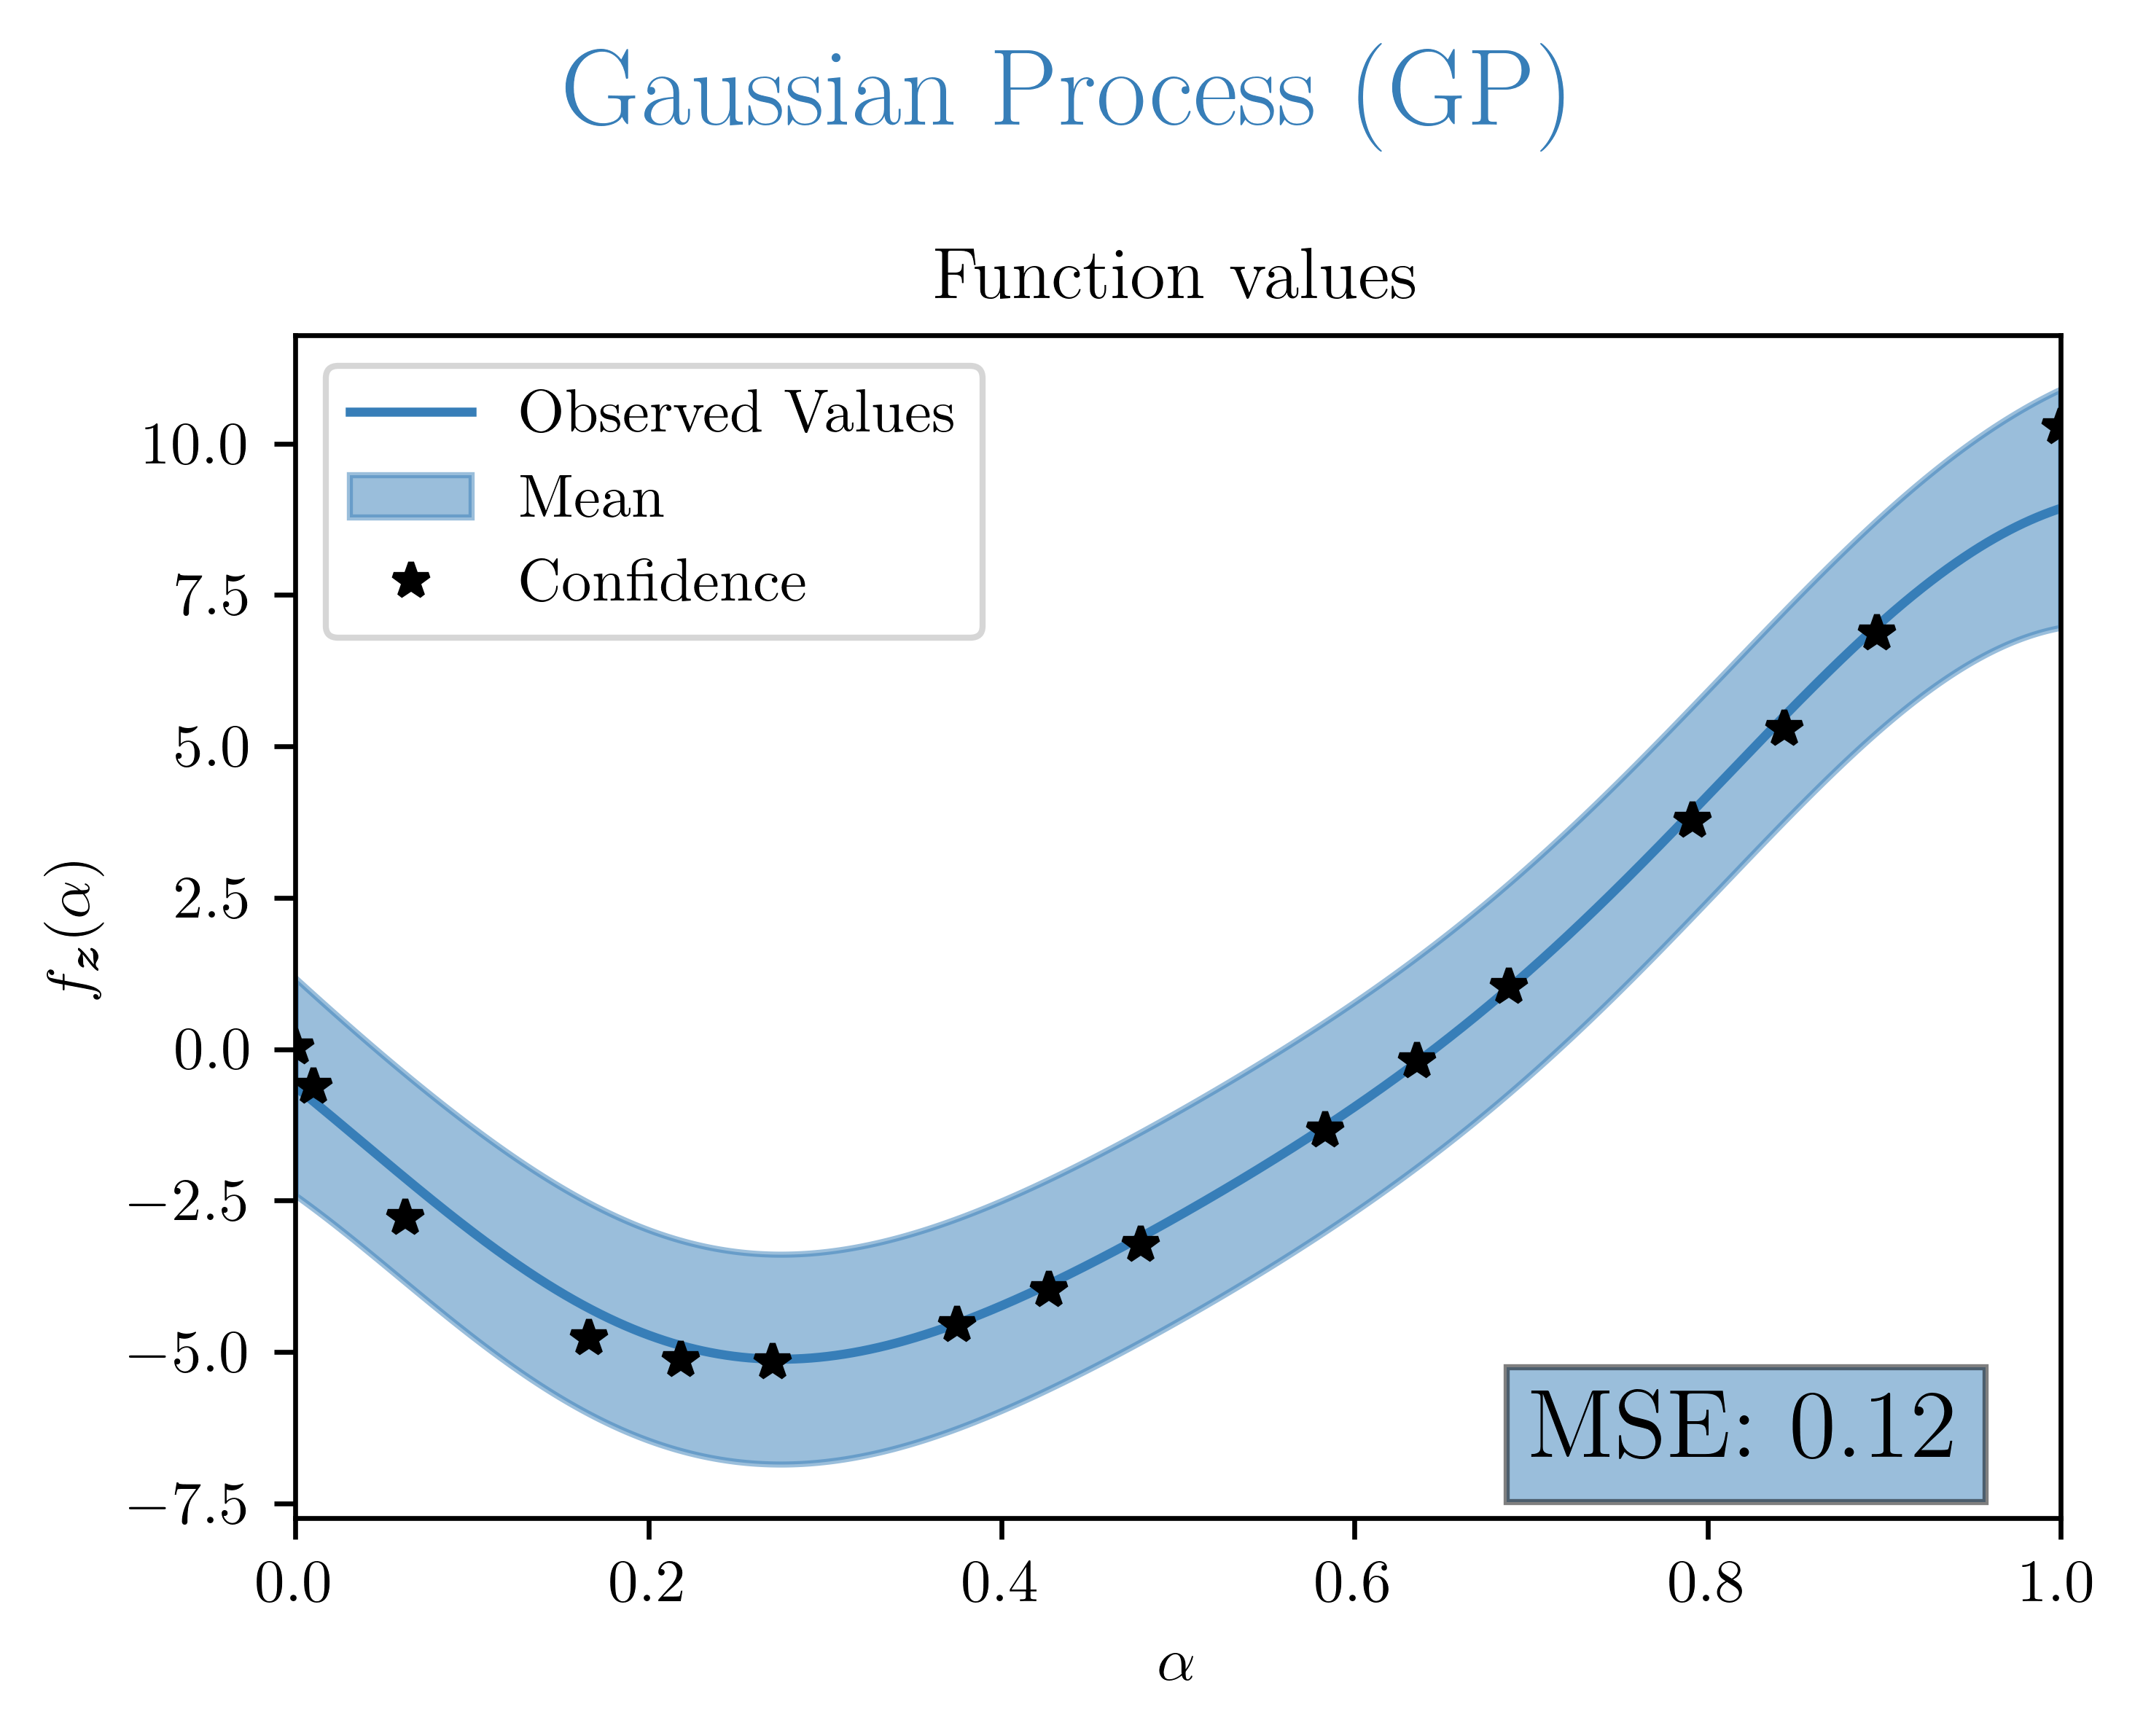
\includegraphics[width=.33\textwidth]{../experiments/uniform_new_MC/GP_16_nobs.png}}{GP with 16 evaluations} & \subf{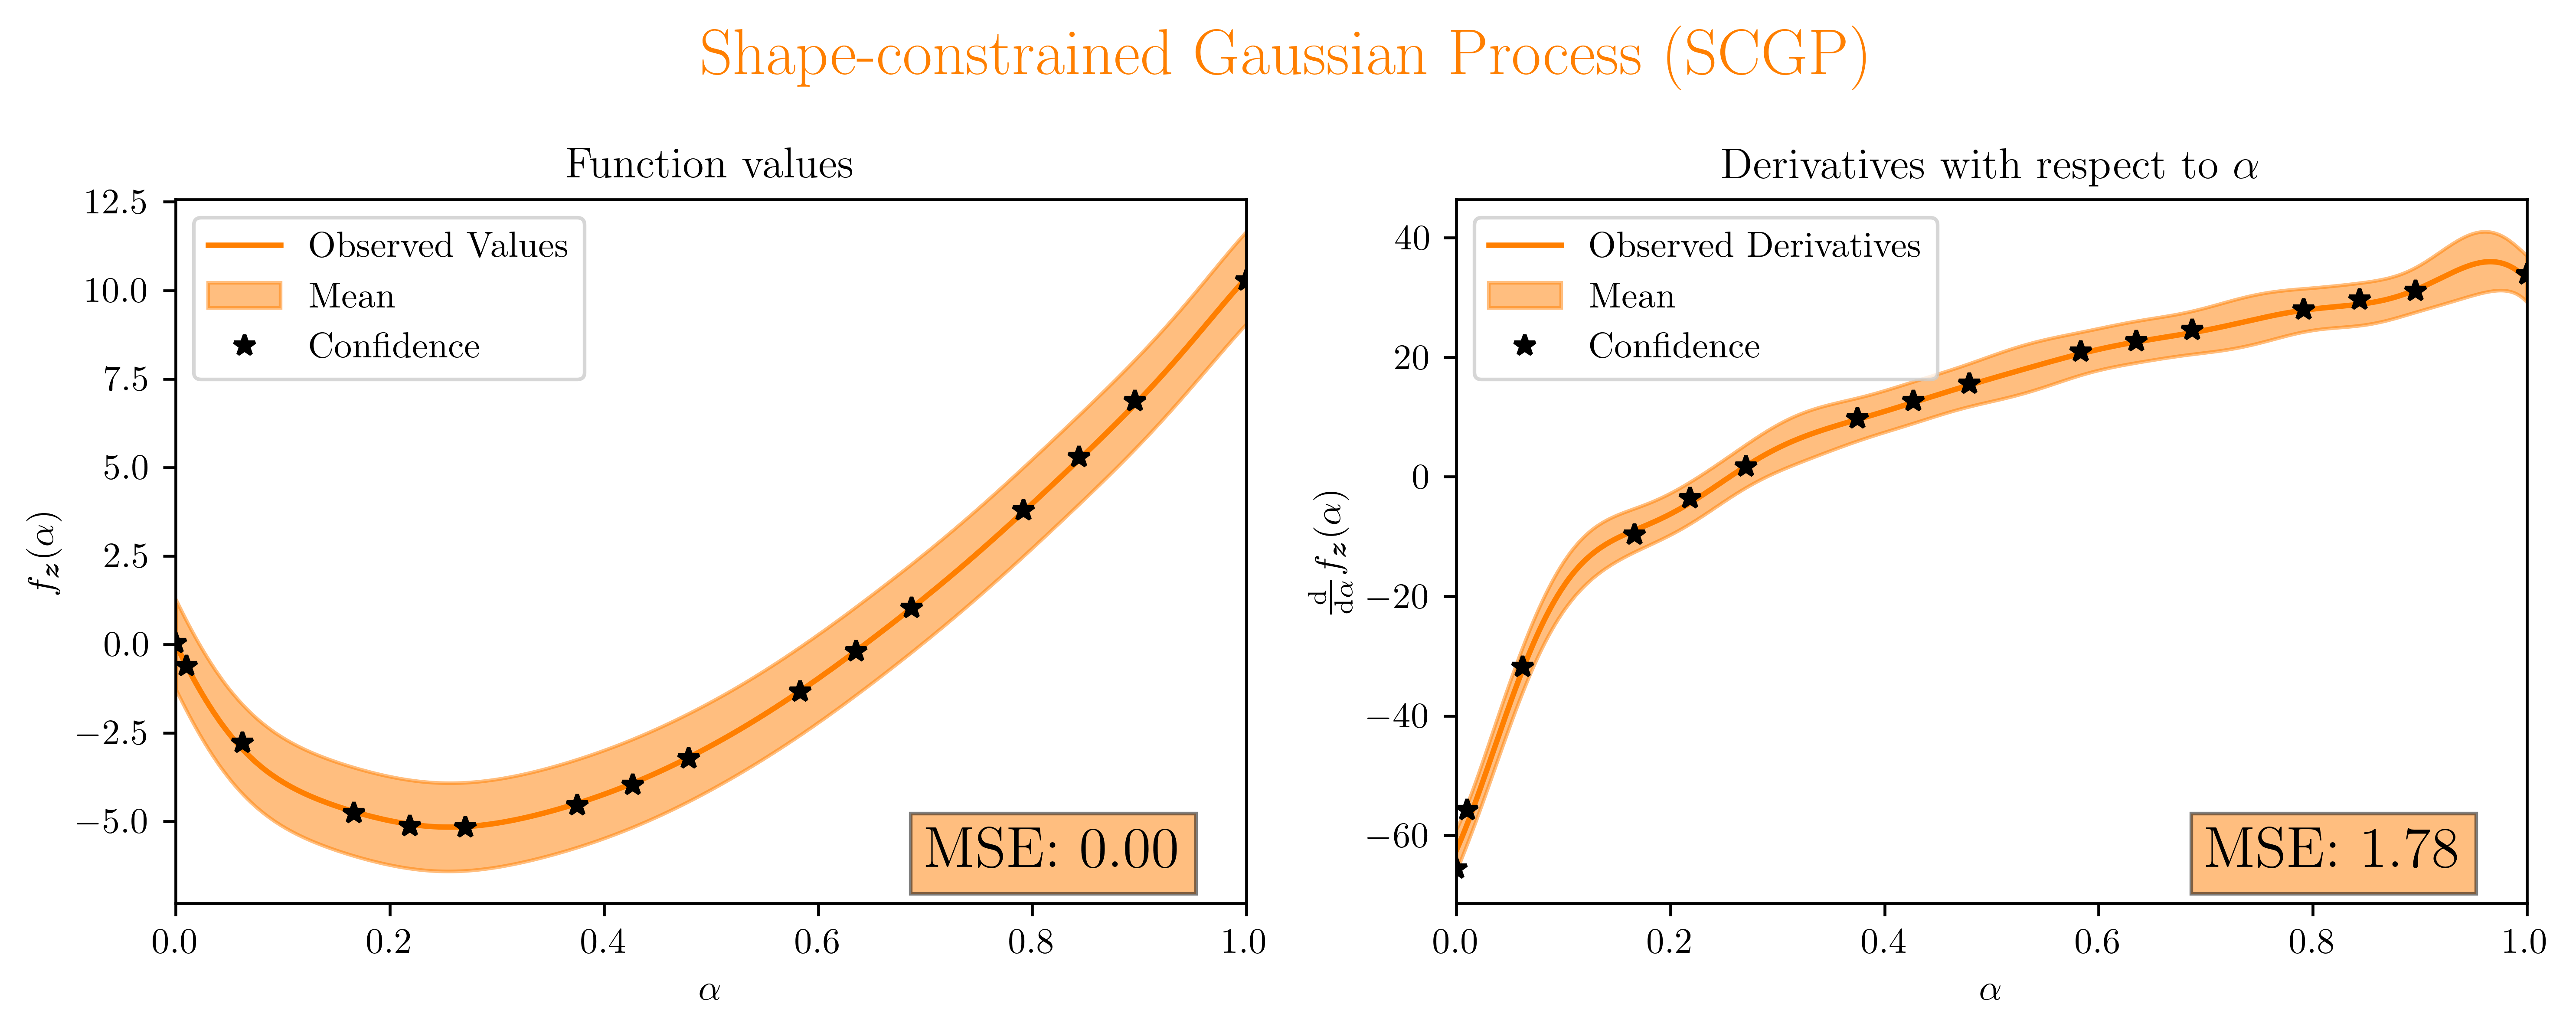
\includegraphics[width=.66\textwidth]{../experiments/uniform_new_MC/SCGP_16_nobs.png}}{SCGP with 16 evaluations} \\
        \hline
        \subf{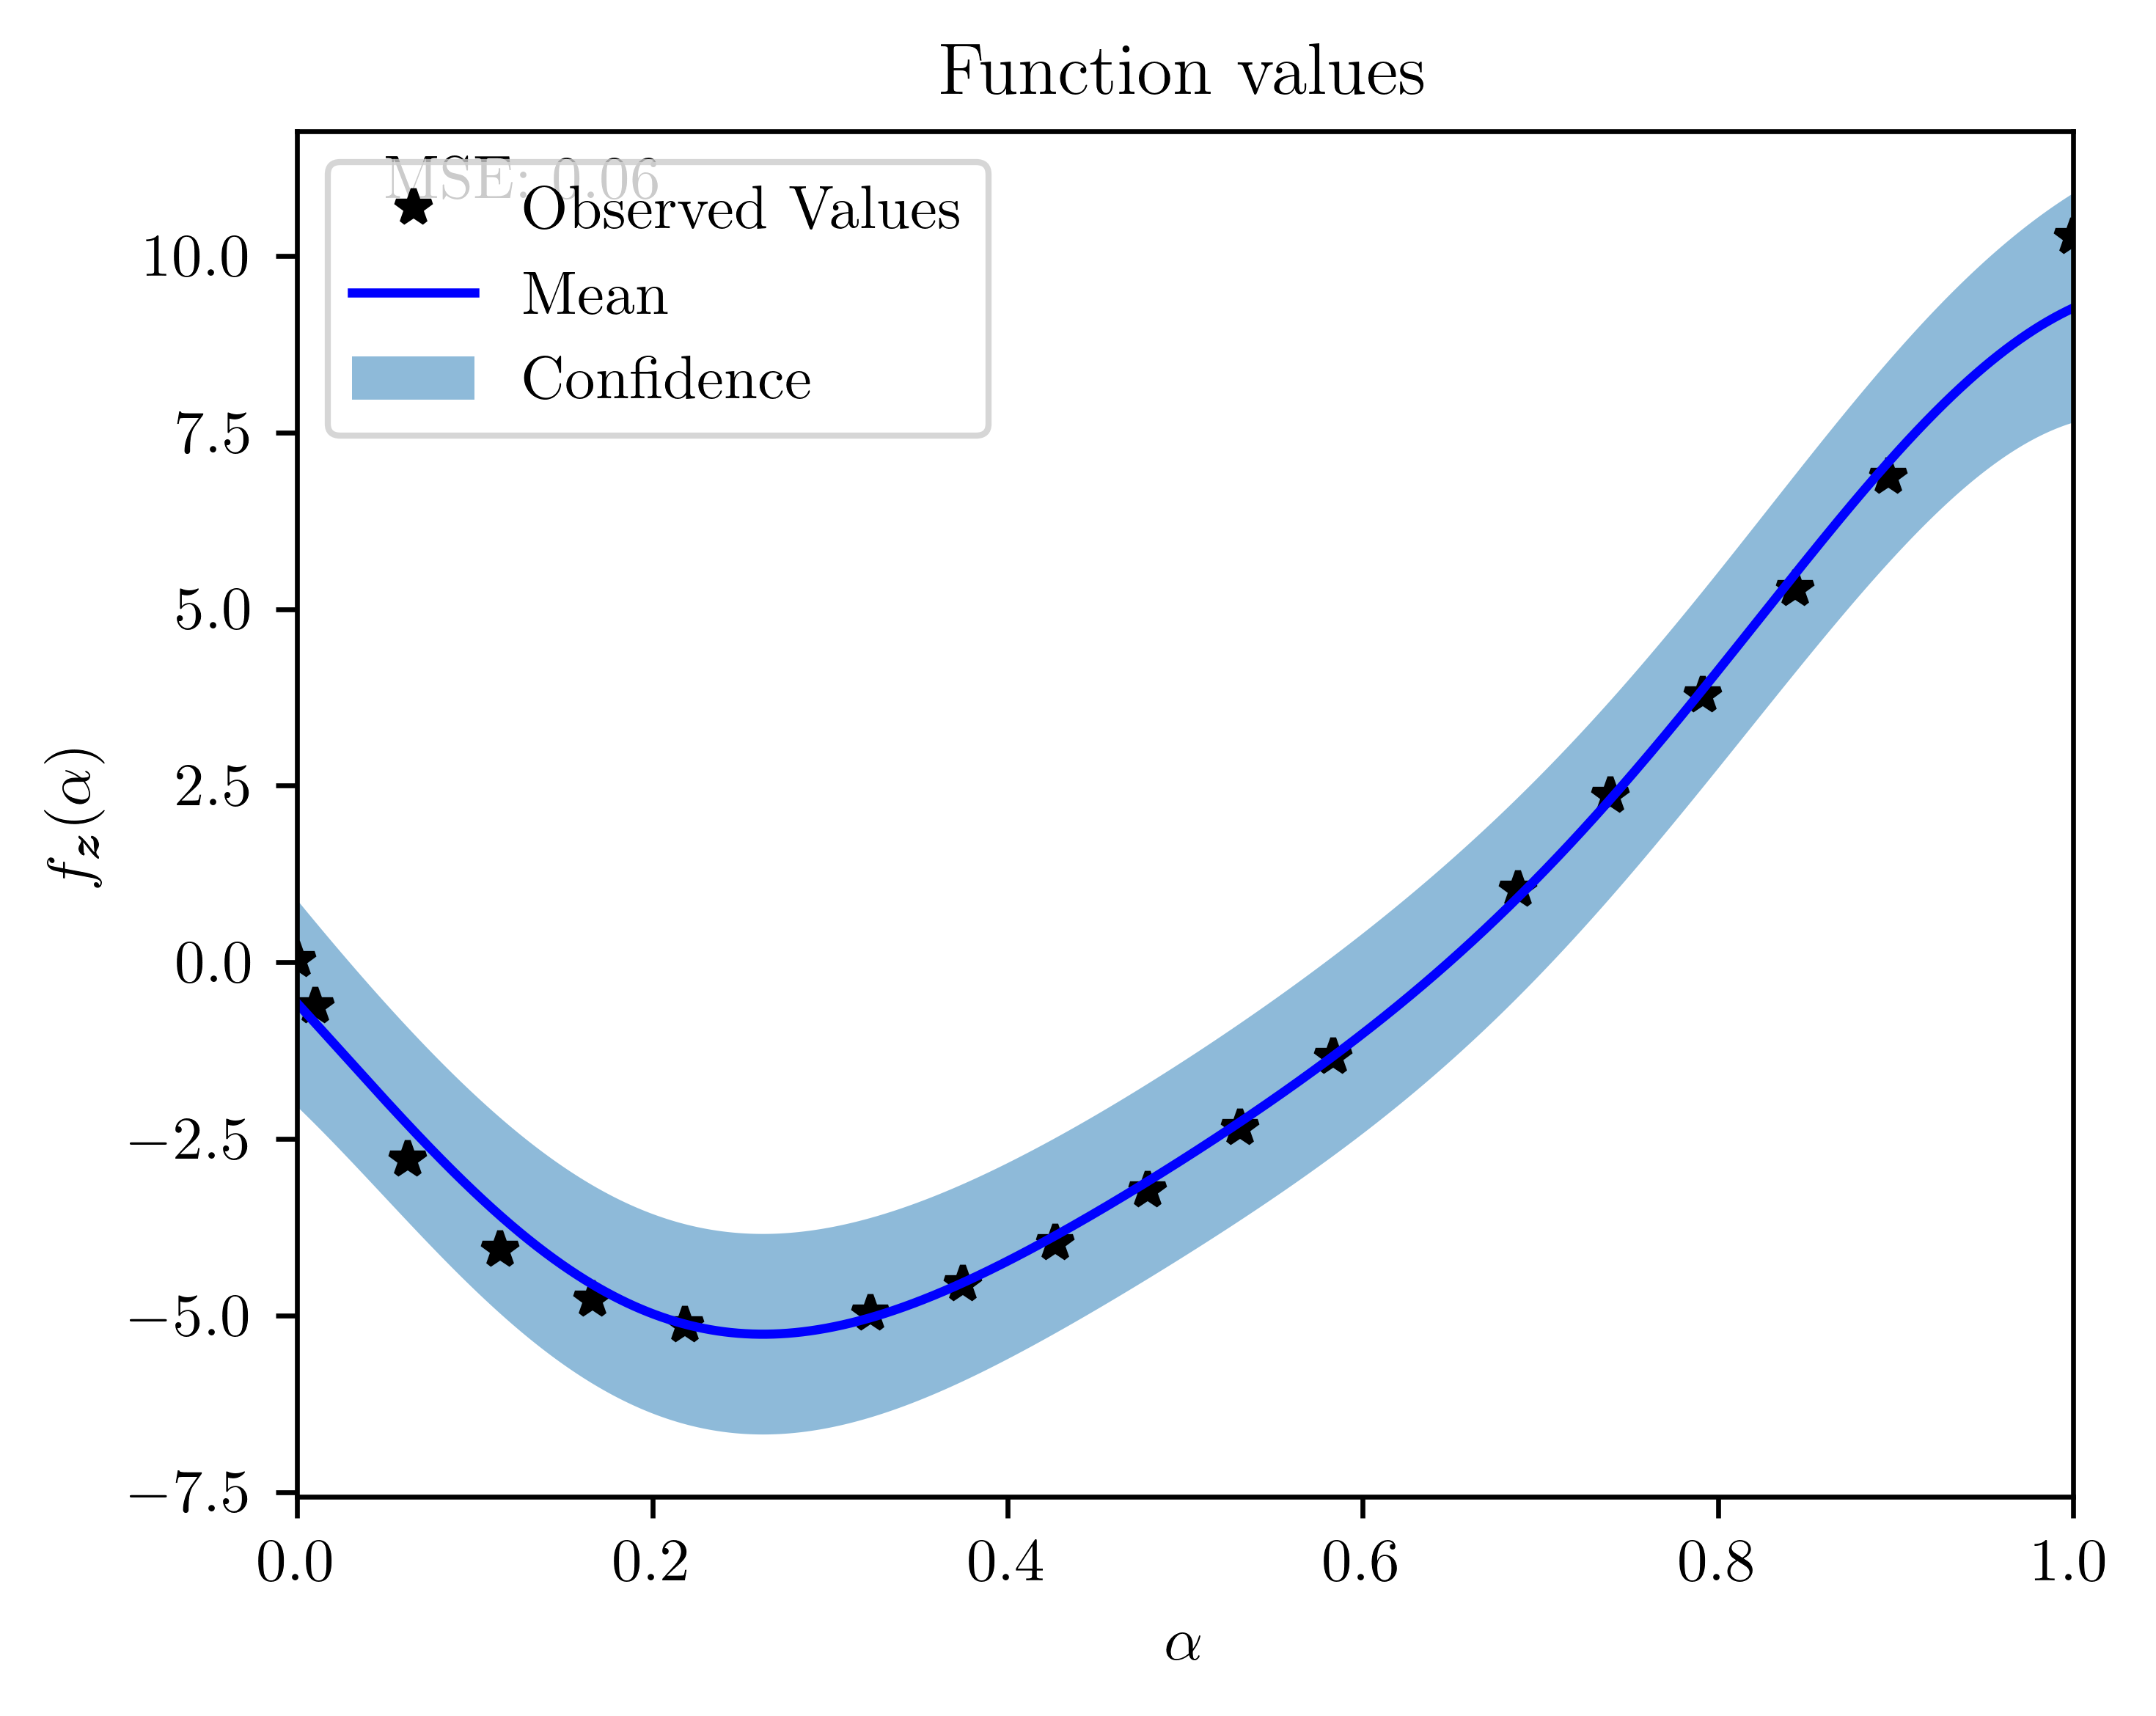
\includegraphics[width=.33\textwidth]{../experiments/uniform_new_MC/GP_18_nobs.png}}{GP with 18 evaluations} & \subf{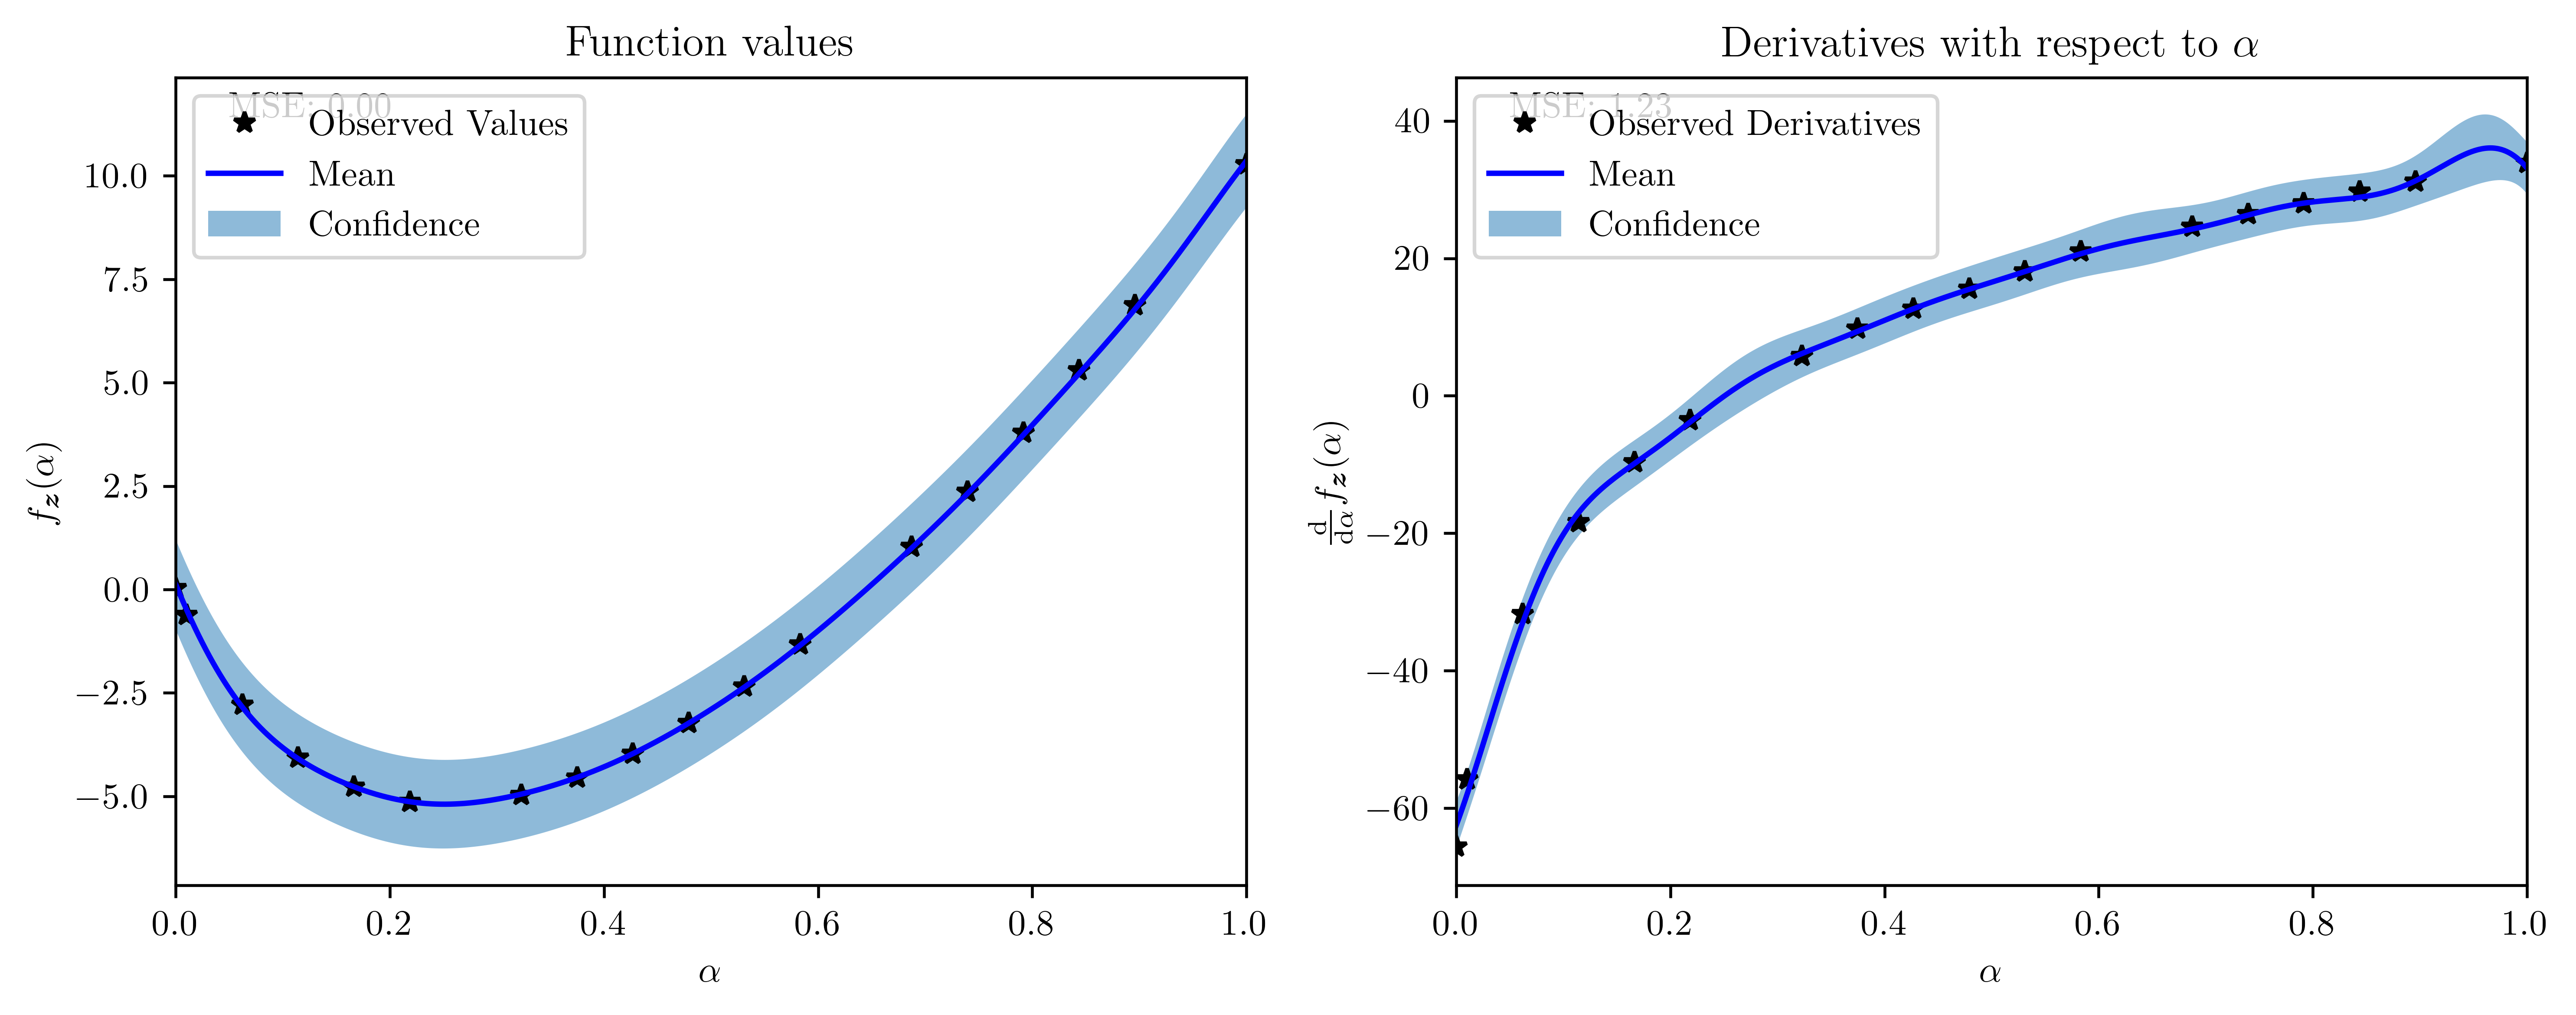
\includegraphics[width=.66\textwidth]{../experiments/uniform_new_MC/SCGP_18_nobs.png}}{SCGP with 18 evaluations} \\
        \hline
    \end{tabular}}
    \caption{ {\small Comparison between Gaussian Process with and without shape constraints under medium curvature and regular grid evaluation (12 to 18 points). Source: author.}}
    \label{fig:reducingMCpt2}
\end{figure}

\subsection{Comparison with SCAM}

Shape Constrained Additive Models (SCAM)~\cite{Pya2014} provide an alternative for incorporating shape constraints in function emulation processes. They extend the concept of GAMs (mentioned in \zcref{sec:gam}) to include shape constraints. The SCAM implementation used here was performed in \texttt{R} with the \texttt{scam} library \cite{scam2012}.

There is no direct uncertainty quantification in SCAM, which is a disadvantage compared to SCGP. In this case, approximate confidence intervals are used through estimators for the standard deviation of each prediction. Note that these confidence intervals cannot be interpreted as Bayesian guarantees and vice versa.

\subsubsection{Variations in Curvature and Position of Observed Values}

We compared the SCGP with the SCAM in the same scenarios of high and medium curvature, evaluated on both regular and irregular grids.

\begin{figure}[H]
    \centering
    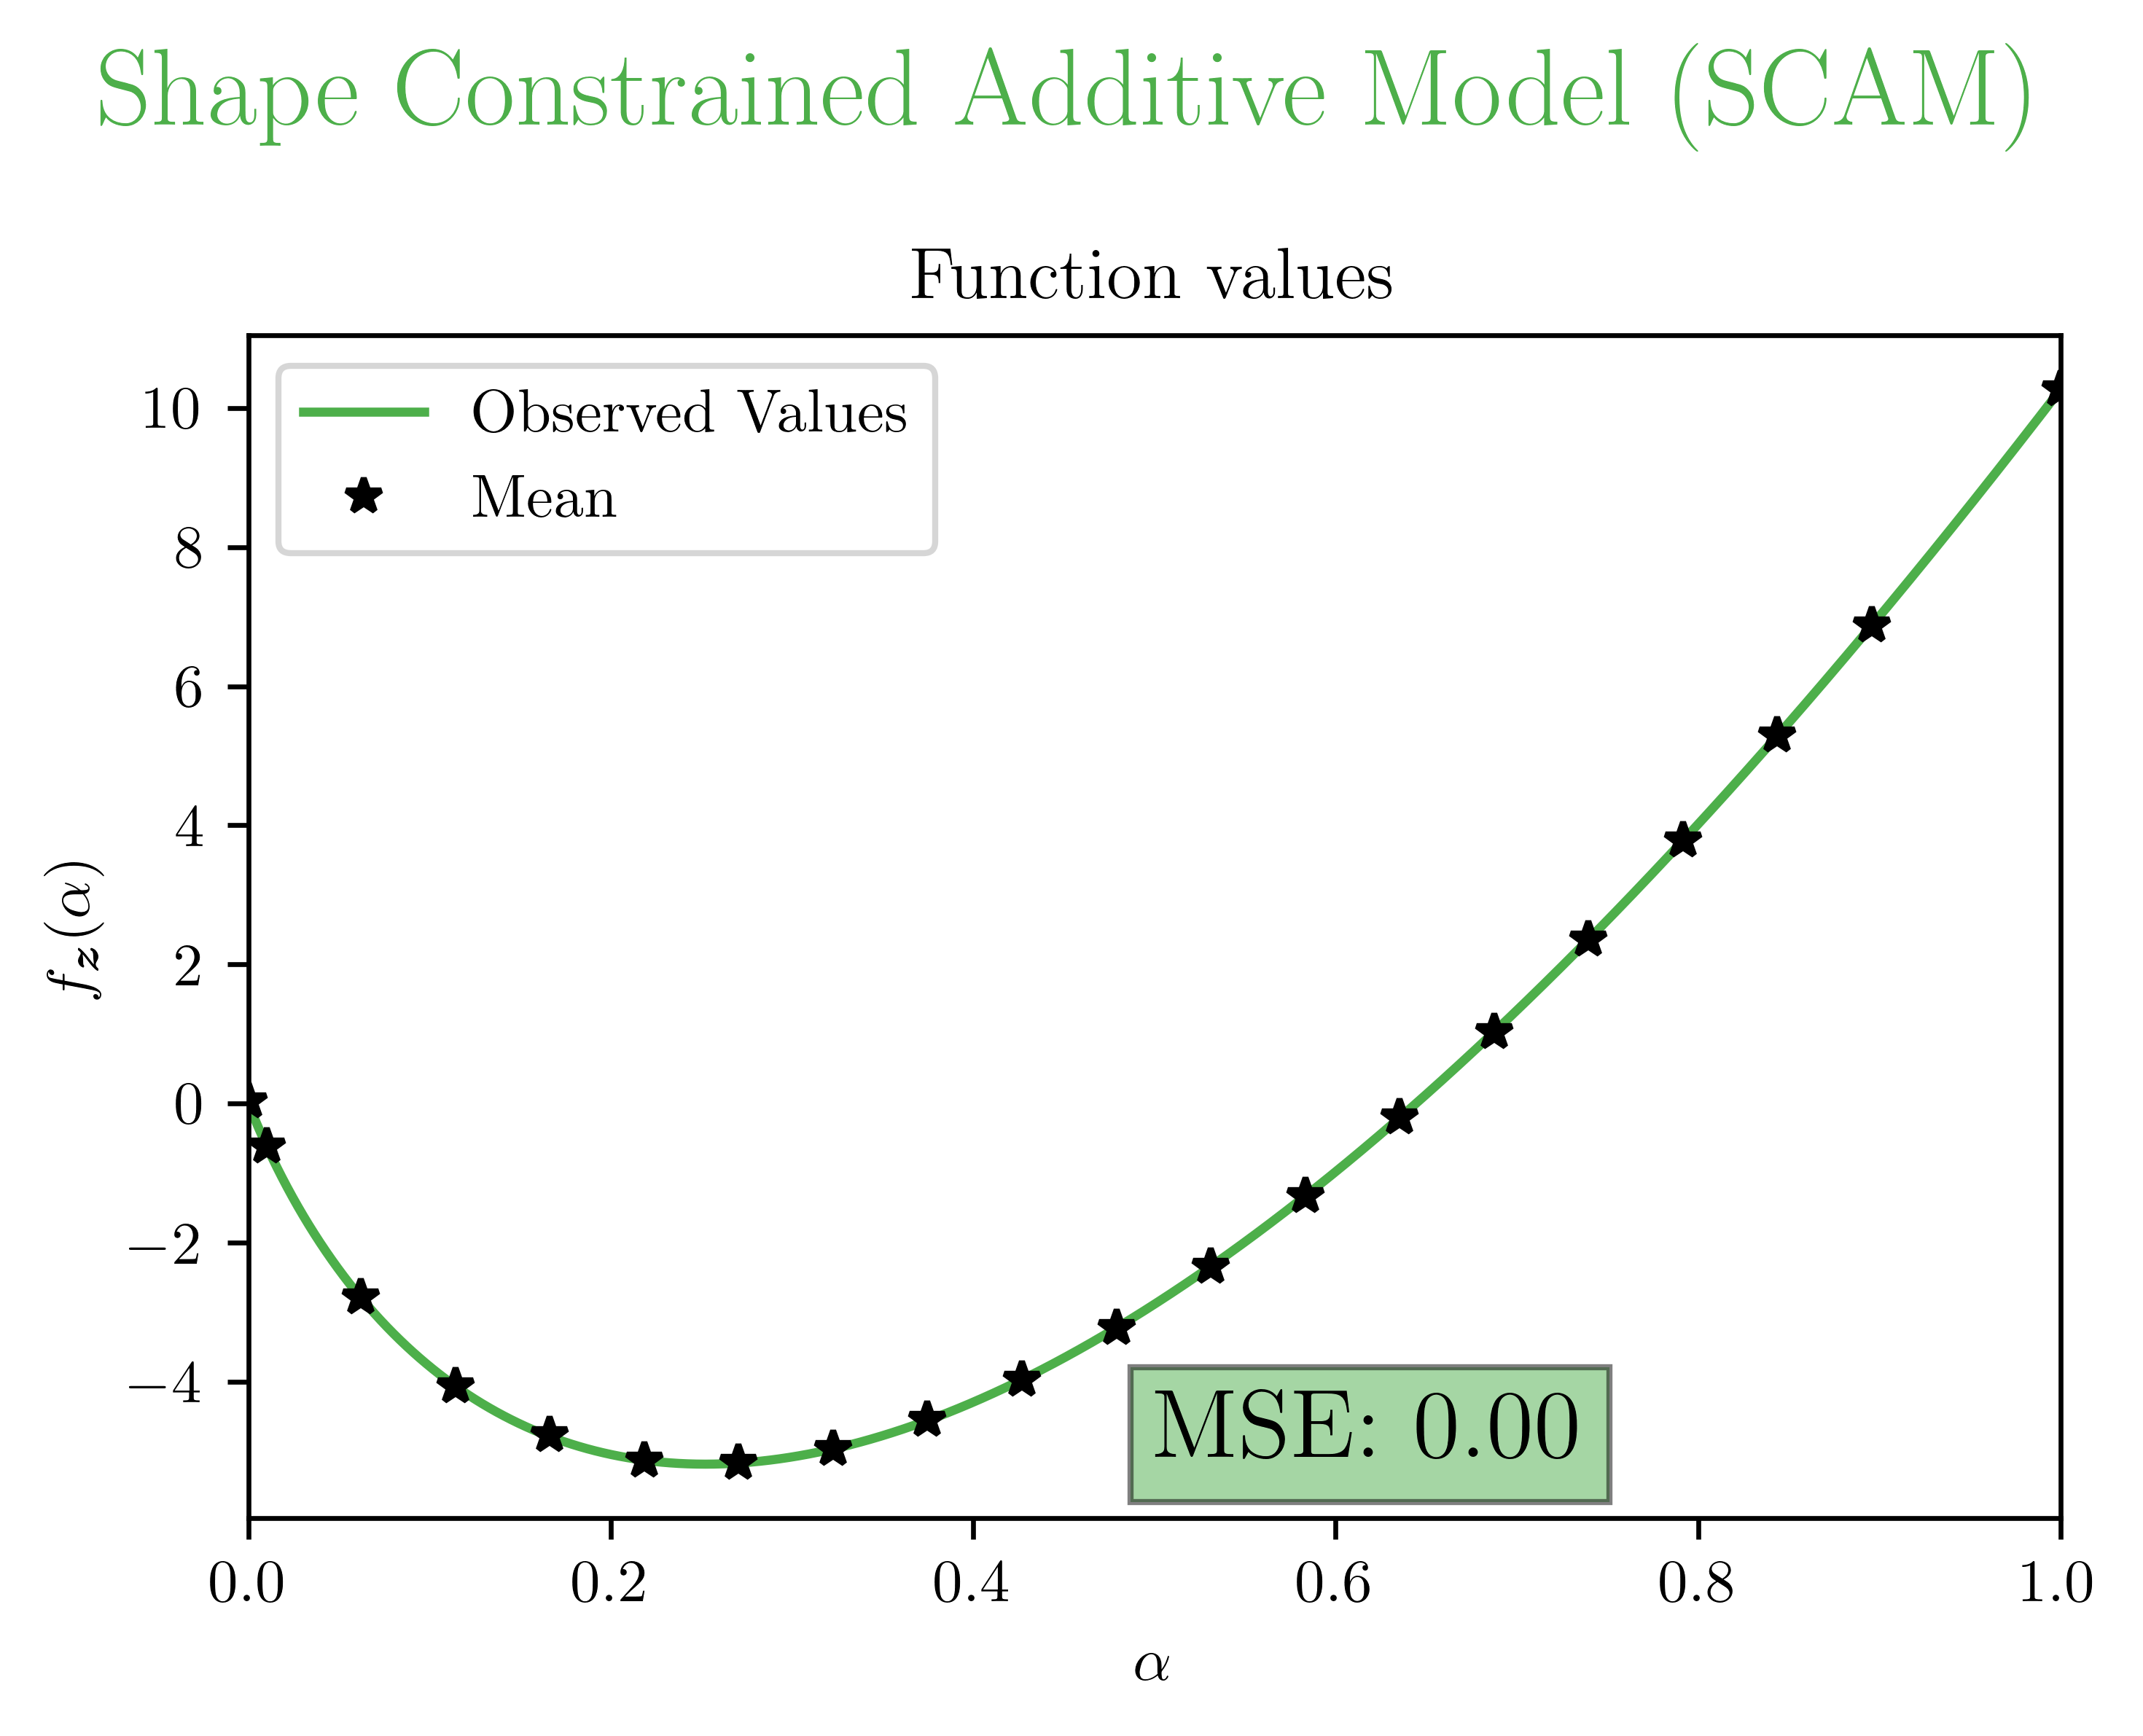
\includegraphics[width=.33\textwidth]{../experiments/uniform_new_MC/SCAM_20_nobs.png}
    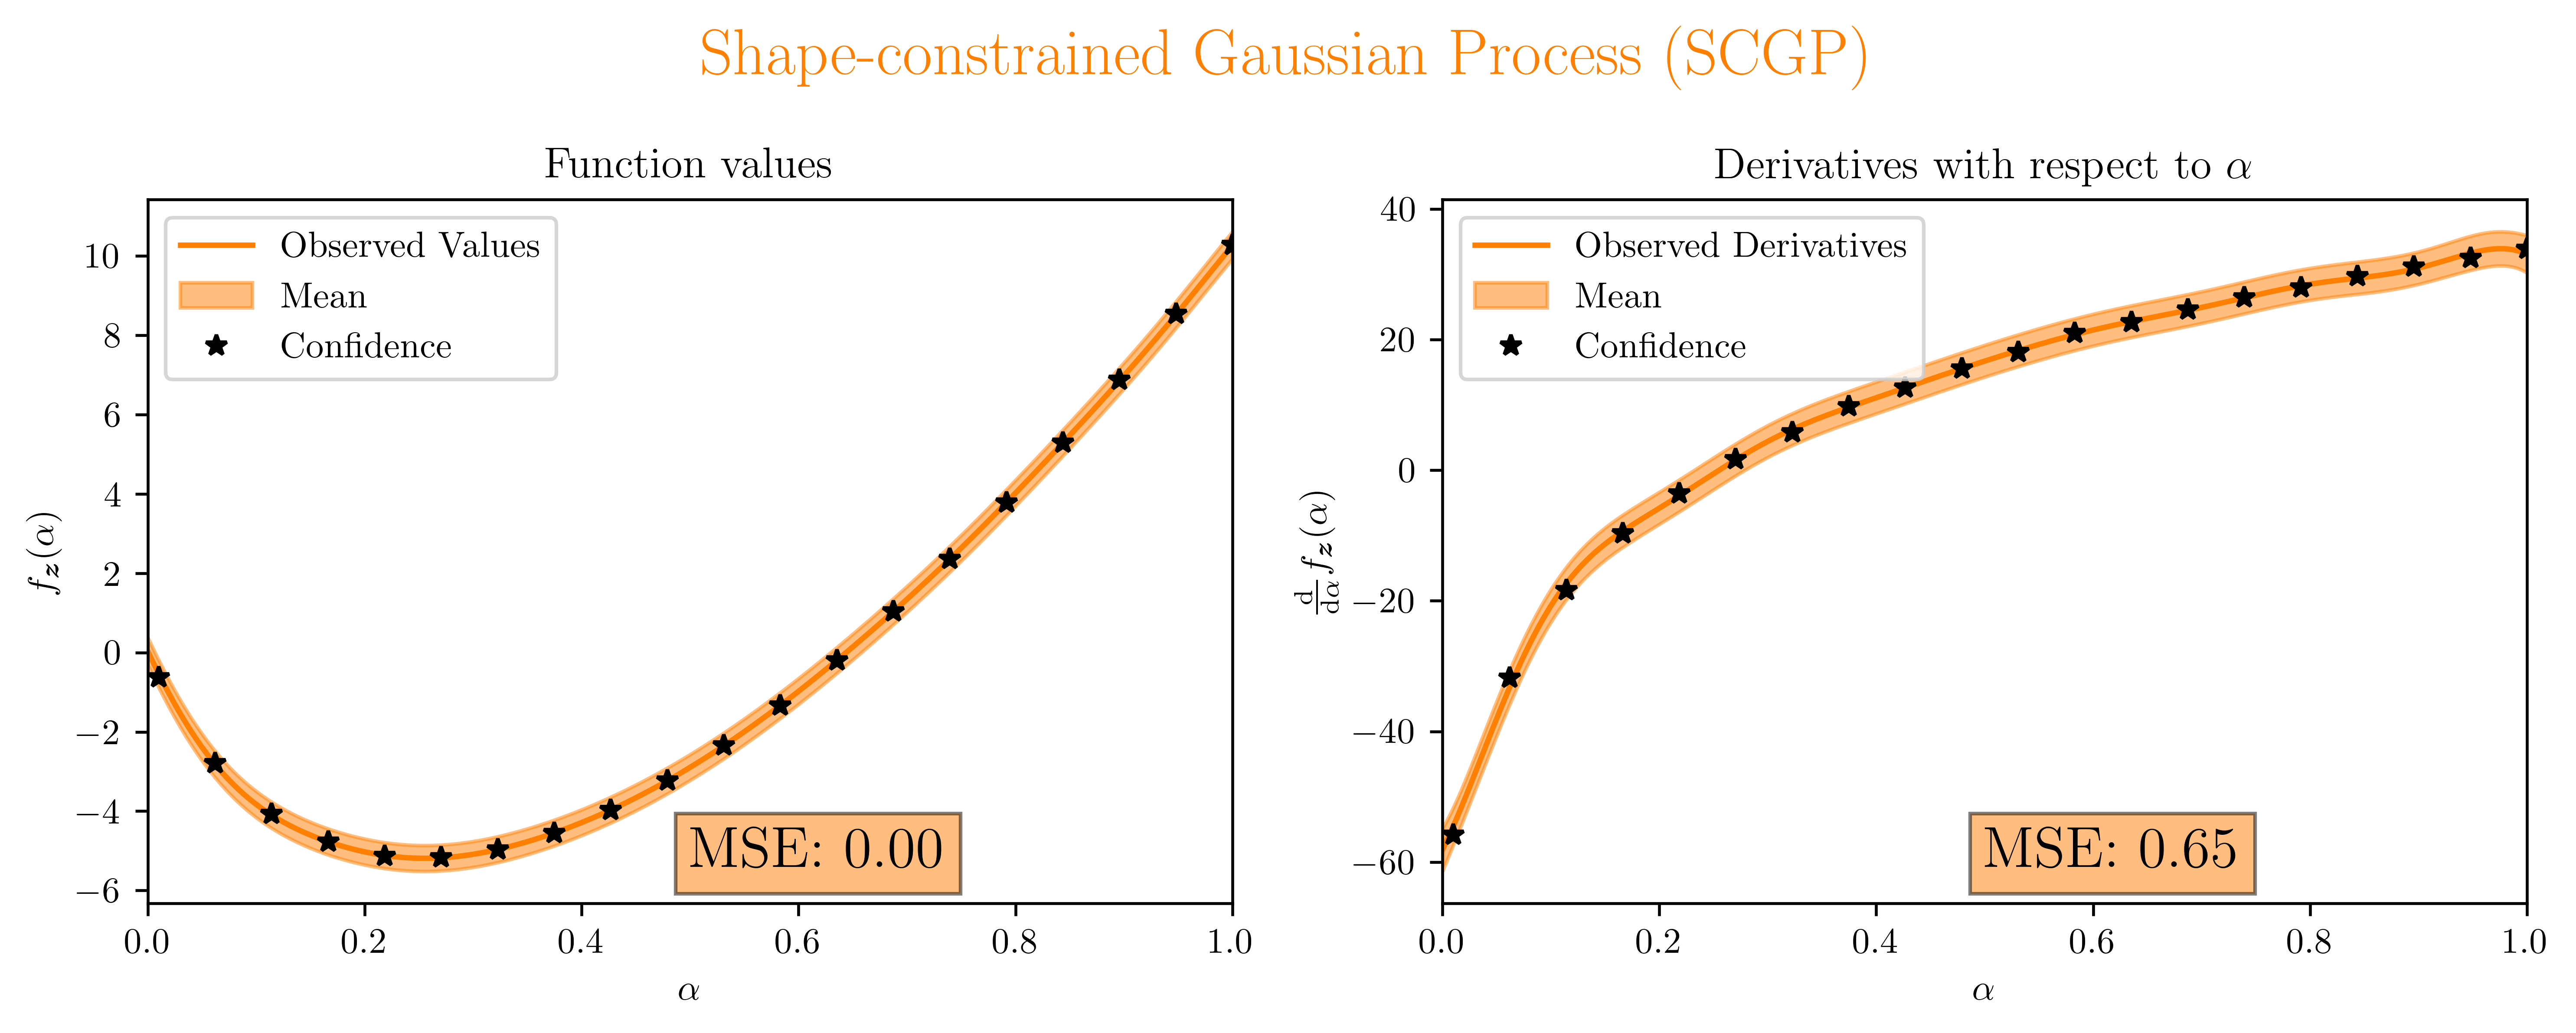
\includegraphics[width=.66\textwidth]{../experiments/uniform_new_MC/SCGP_20_nobs.png}
    \caption{ {\small Comparison between SCAM and SCGP under medium curvature and regular grid evaluation. Source: author.}}
    \label{fig:SCAMuniformMC}
\end{figure}

Observing \zcref{fig:SCAMuniformMC}, we see that both methods performed well in capturing the curvature of the function \( f_{\bfz}(\alpha) \).

\begin{figure}[H]
    \centering
    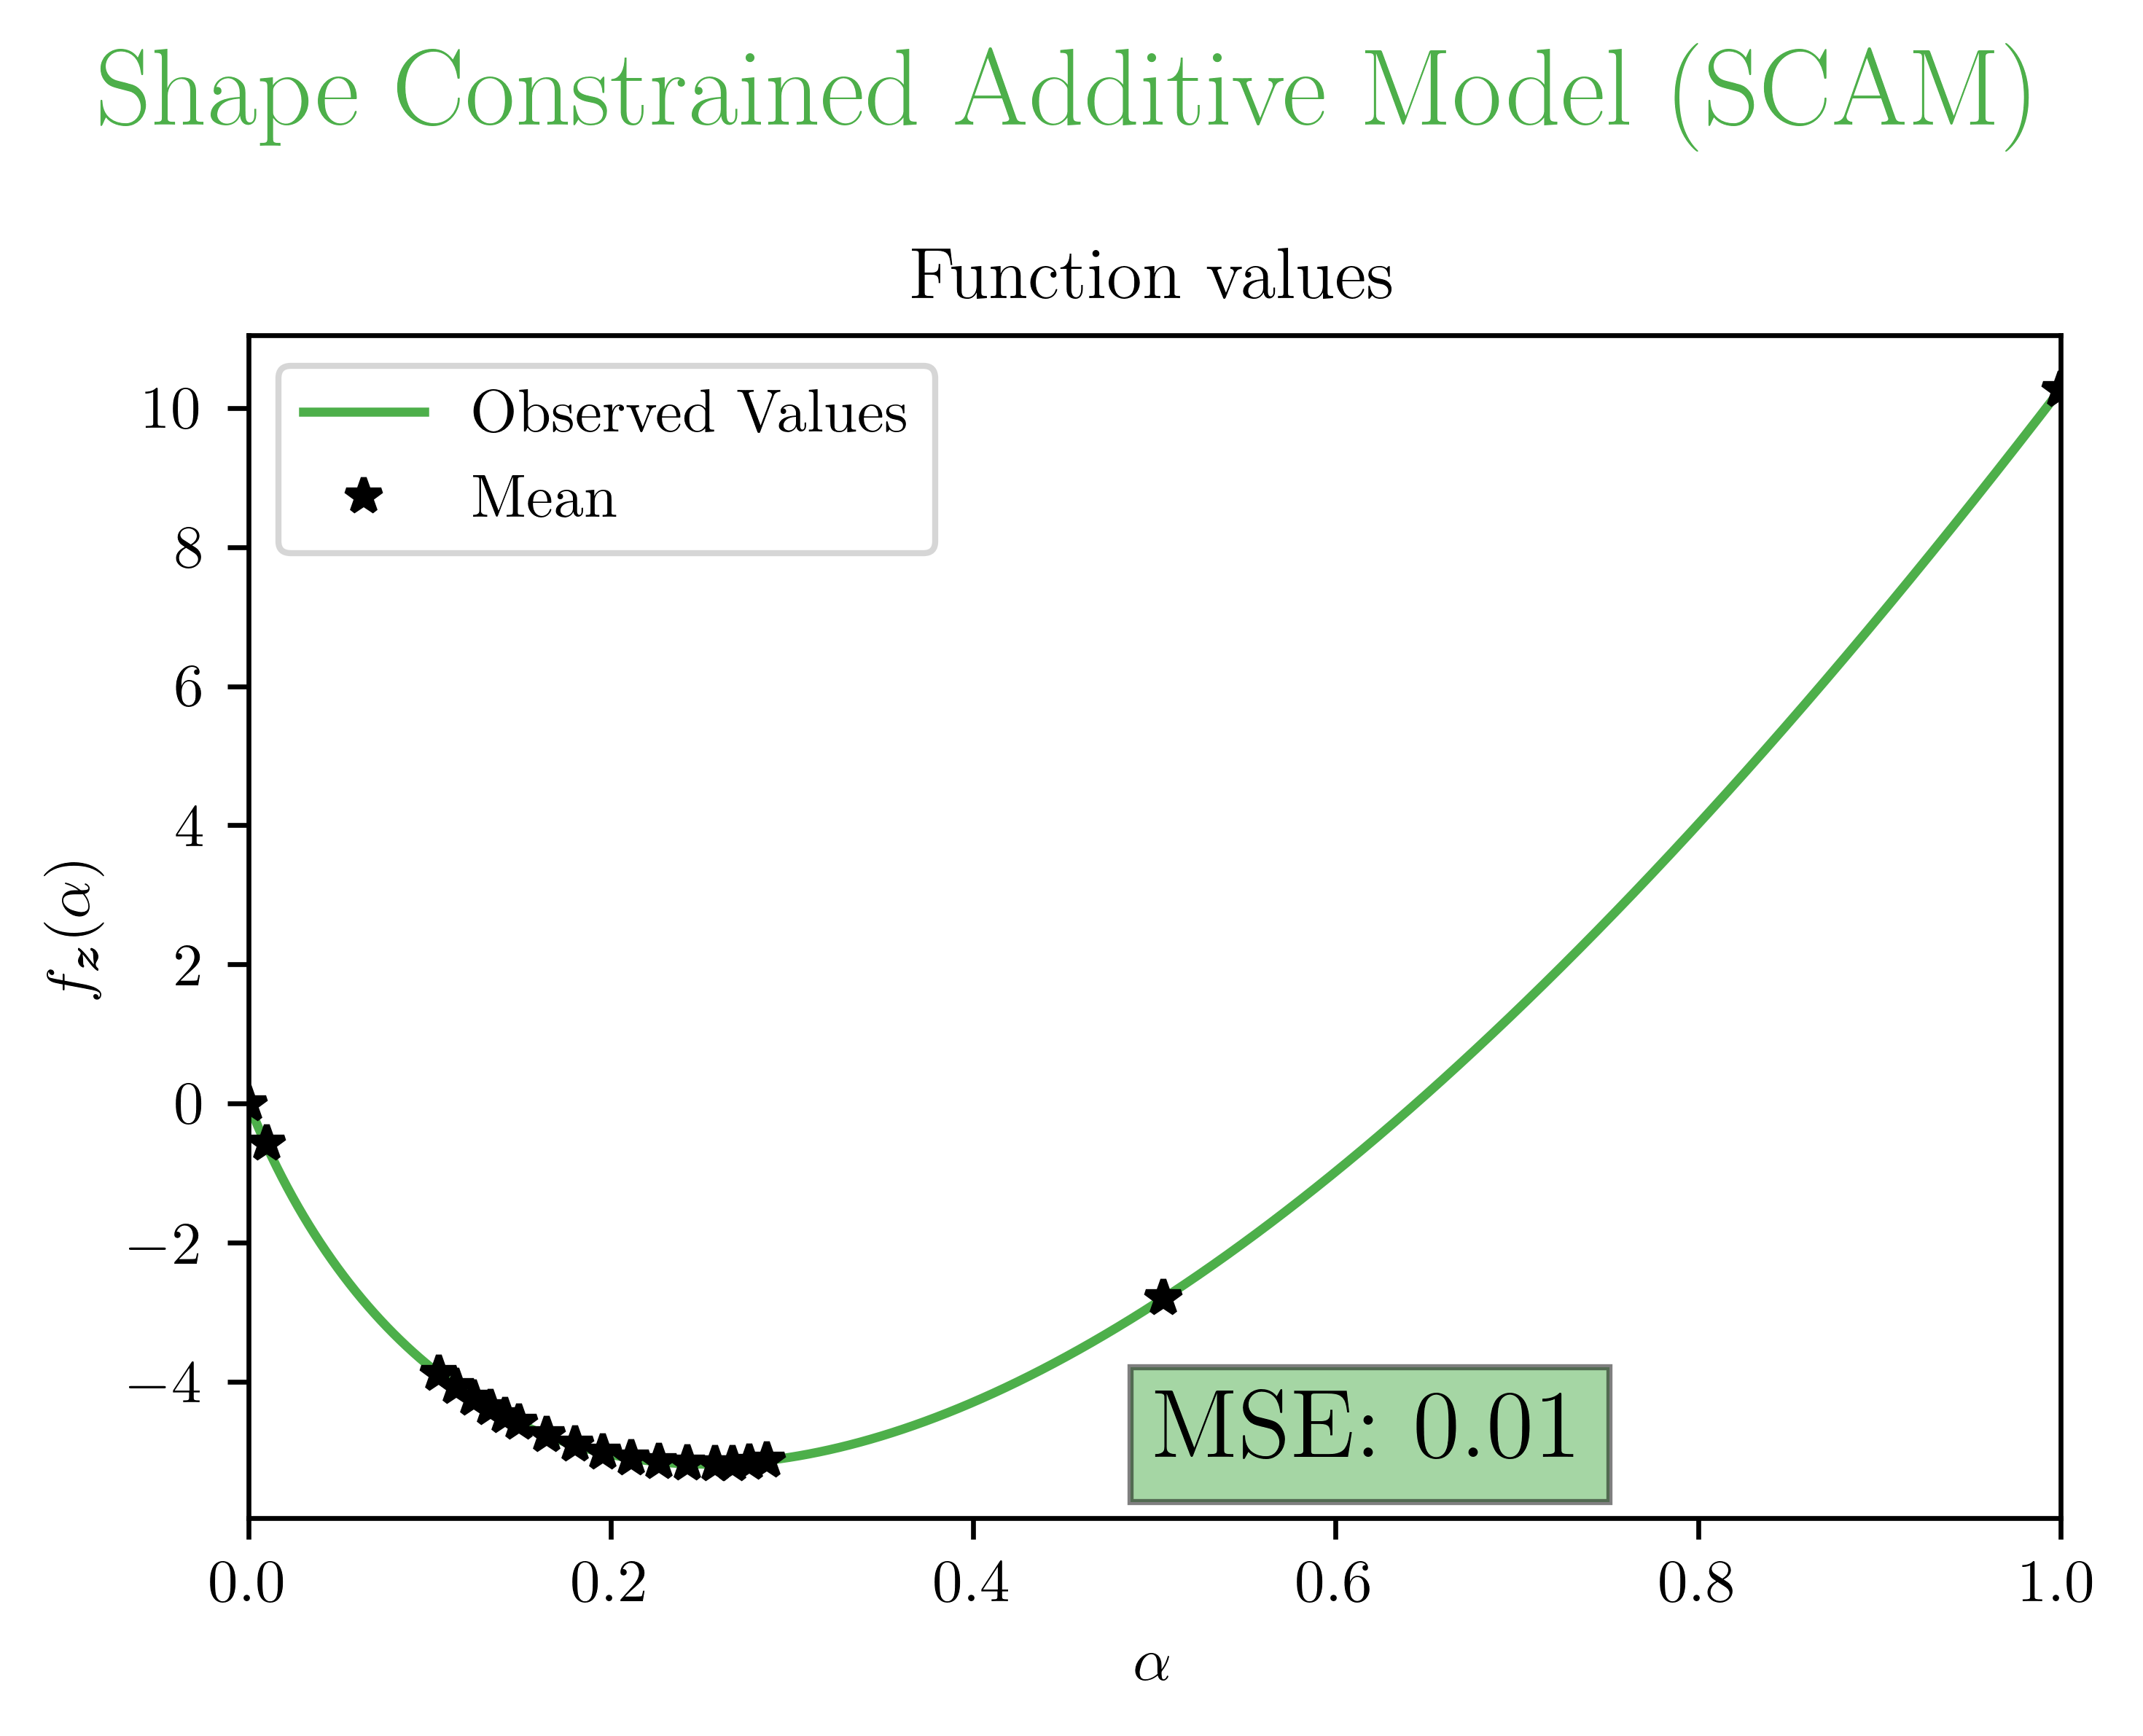
\includegraphics[width=.33\textwidth]{../experiments/adaptive_new_MC/SCAM_20_nobs.png}
    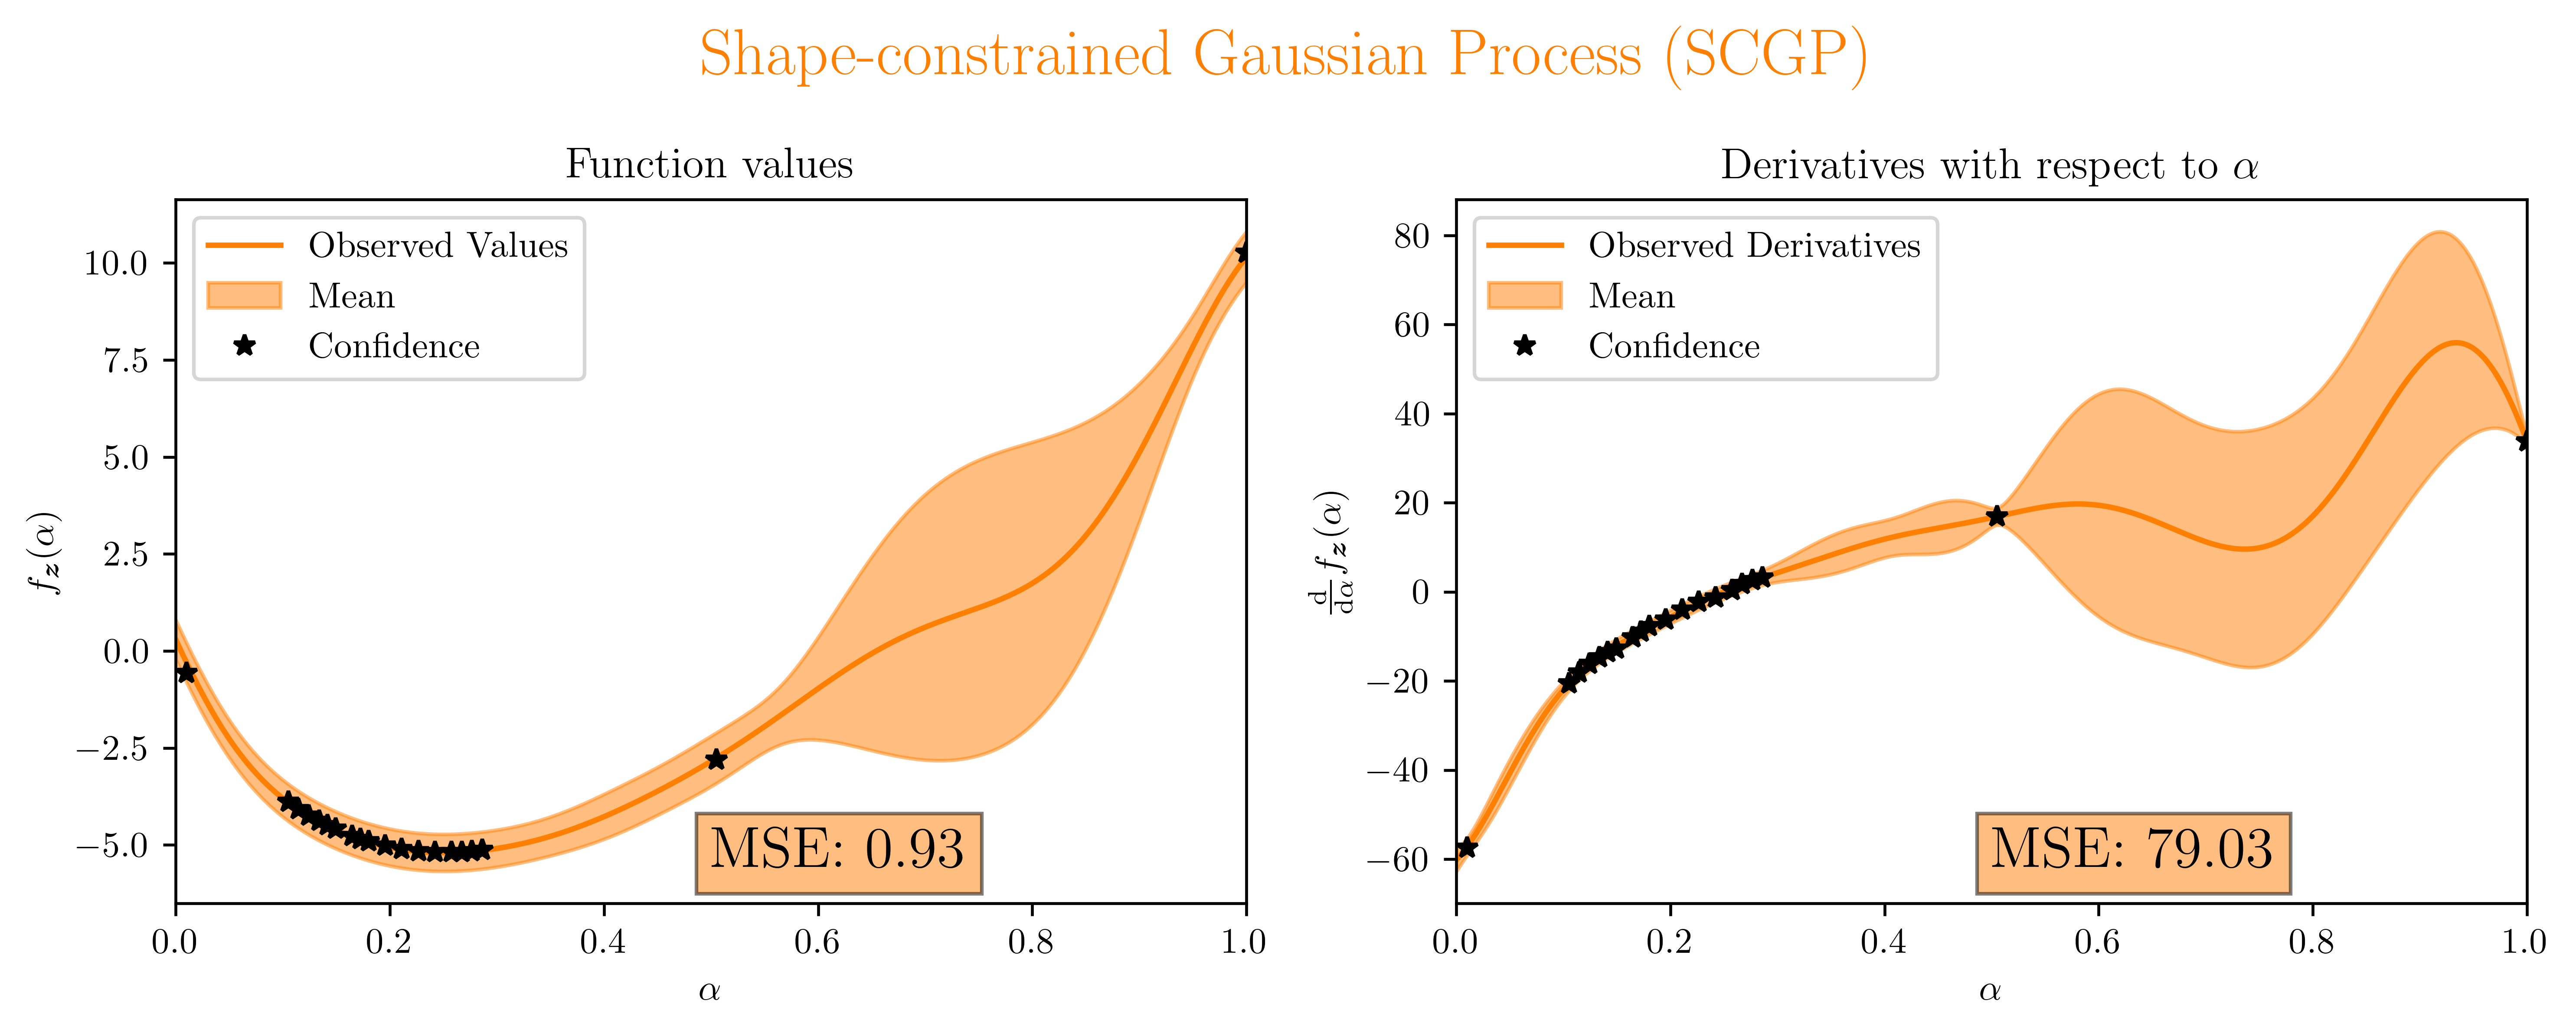
\includegraphics[width=.66\textwidth]{../experiments/adaptive_new_MC/SCGP_20_nobs.png}
    \caption{ {\small Comparison between SCAM and SCGP under medium curvature and irregular grid evaluation. Source: author.}}
    \label{fig:SCAMadaptiveMC}
\end{figure}

In the case of irregular grid evaluation, \zcref{fig:SCAMadaptiveMC} shows that SCAM was effective in capturing the curvature of the function \( f_{\bfz}(\alpha) \), whereas the SCGP did not provide a satisfactory fit.

\begin{figure}[H]
    \centering
    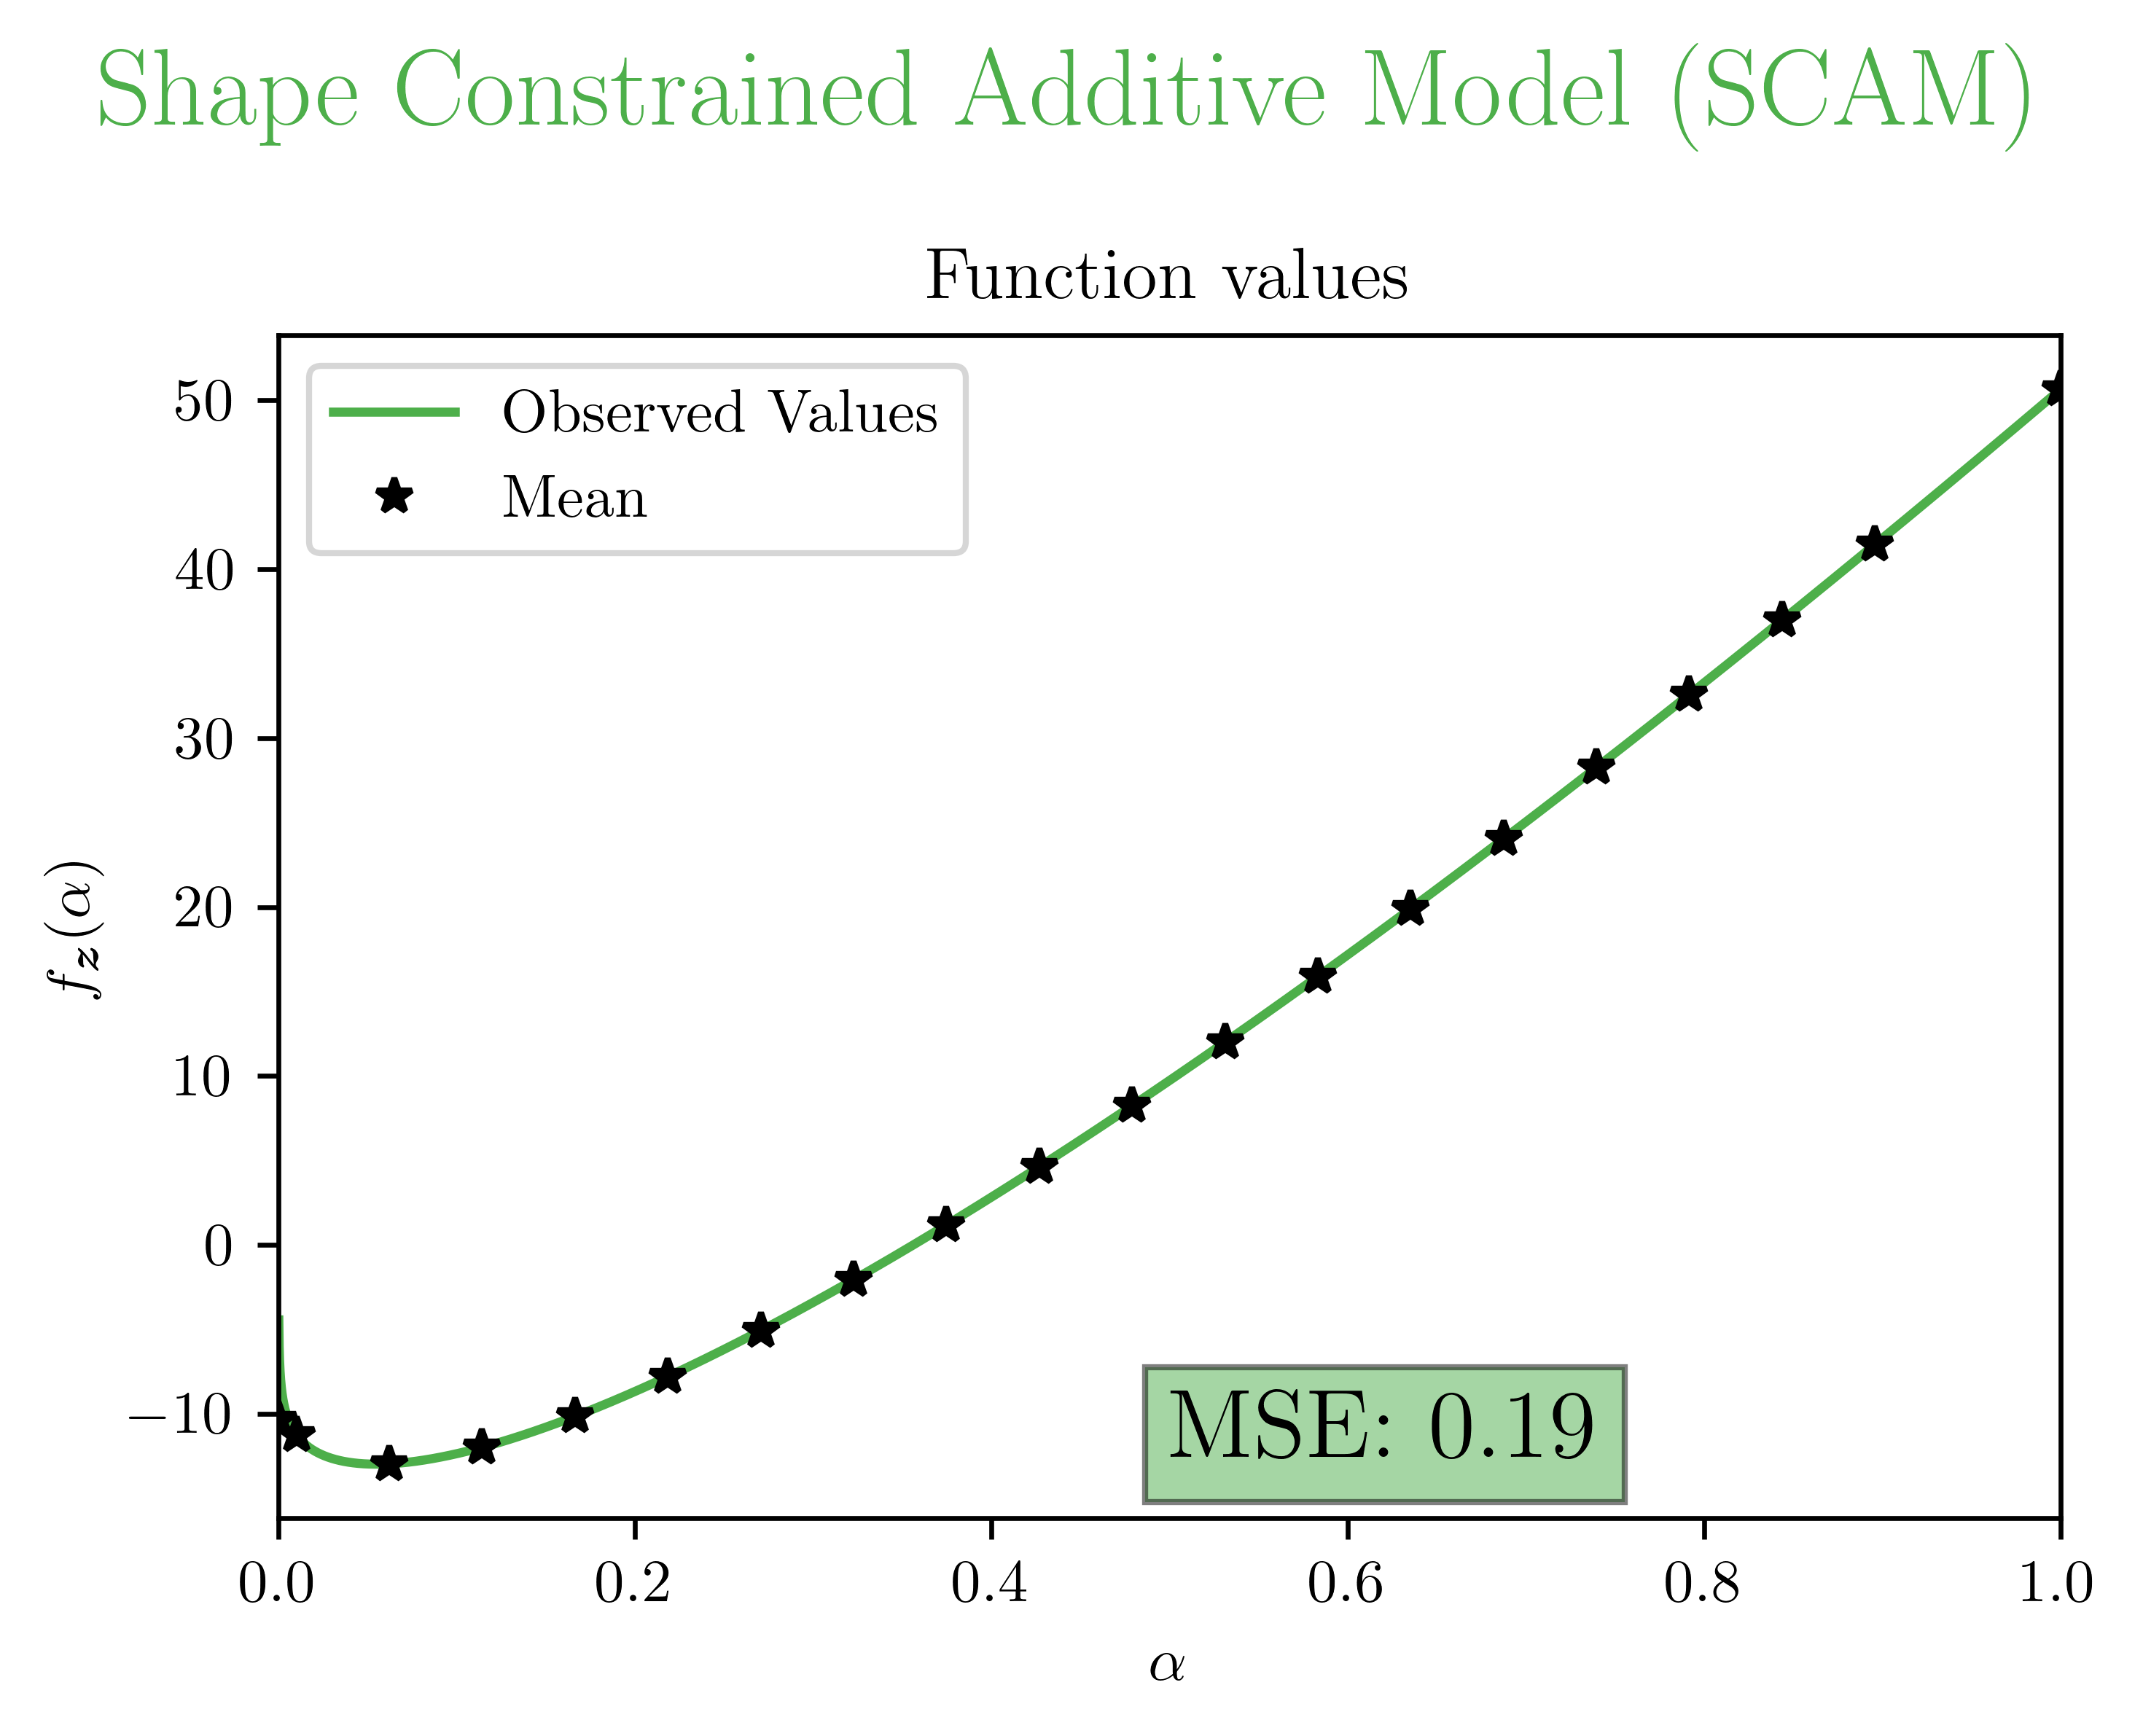
\includegraphics[width=.33\textwidth]{../experiments/uniform_new_HC/SCAM_20_nobs.png}
    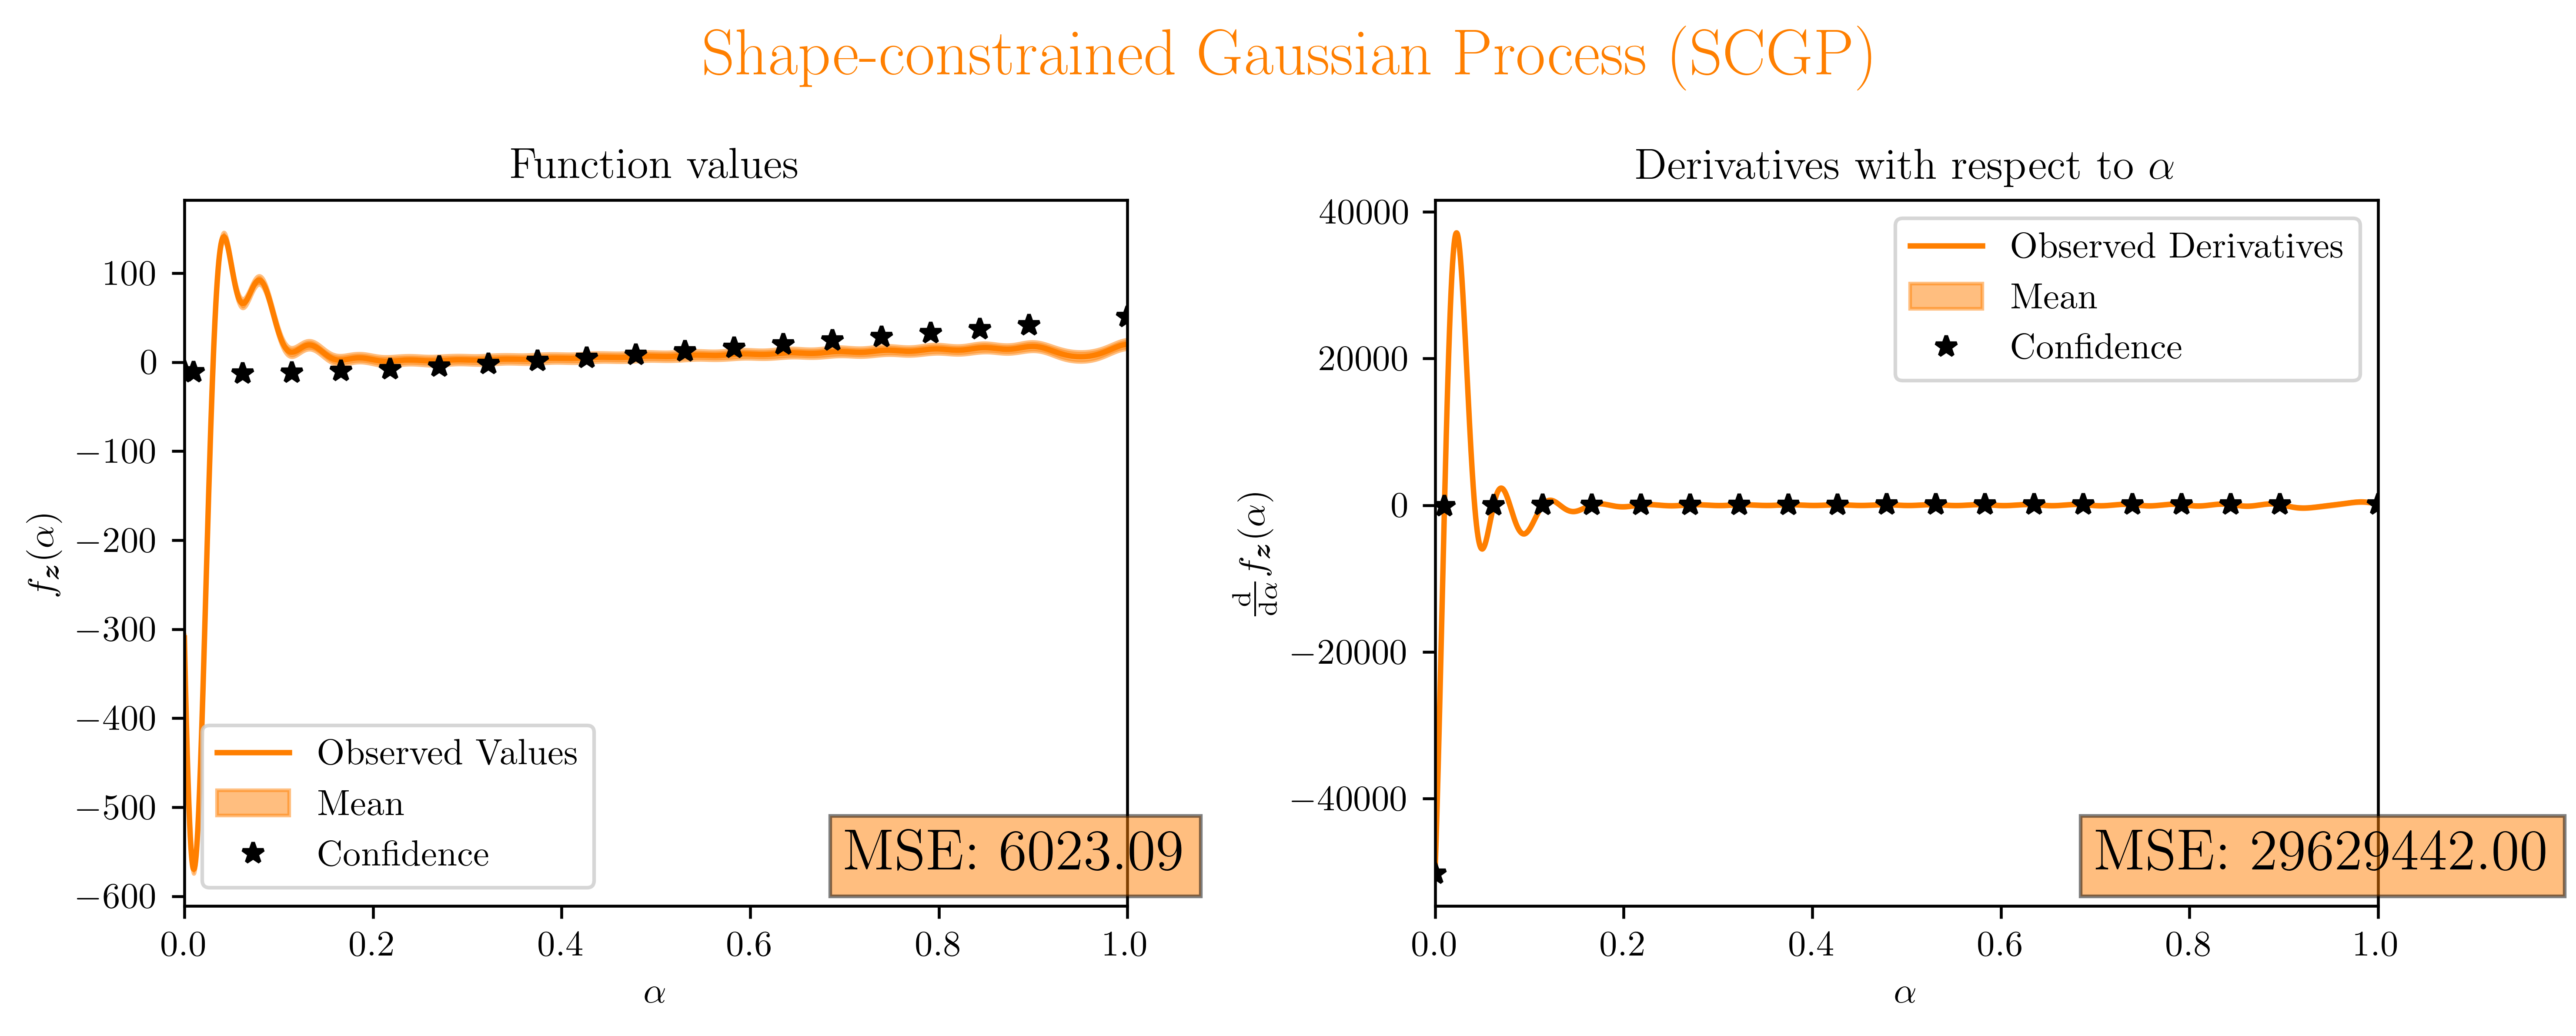
\includegraphics[width=.66\textwidth]{../experiments/uniform_new_HC/SCGP_20_nobs.png}
    \caption{ {\small Comparison between SCAM and SCGP under high curvature and regular grid evaluation. Source: author.}}
    \label{fig:SCAMuniformHC}
\end{figure}

In \zcref{fig:SCAMuniformHC}, although the SCGP manages to adequately recover the target curvature, it is outperformed by the SCAM, which nearly interpolates the function.

\begin{figure}[H]
    \centering
    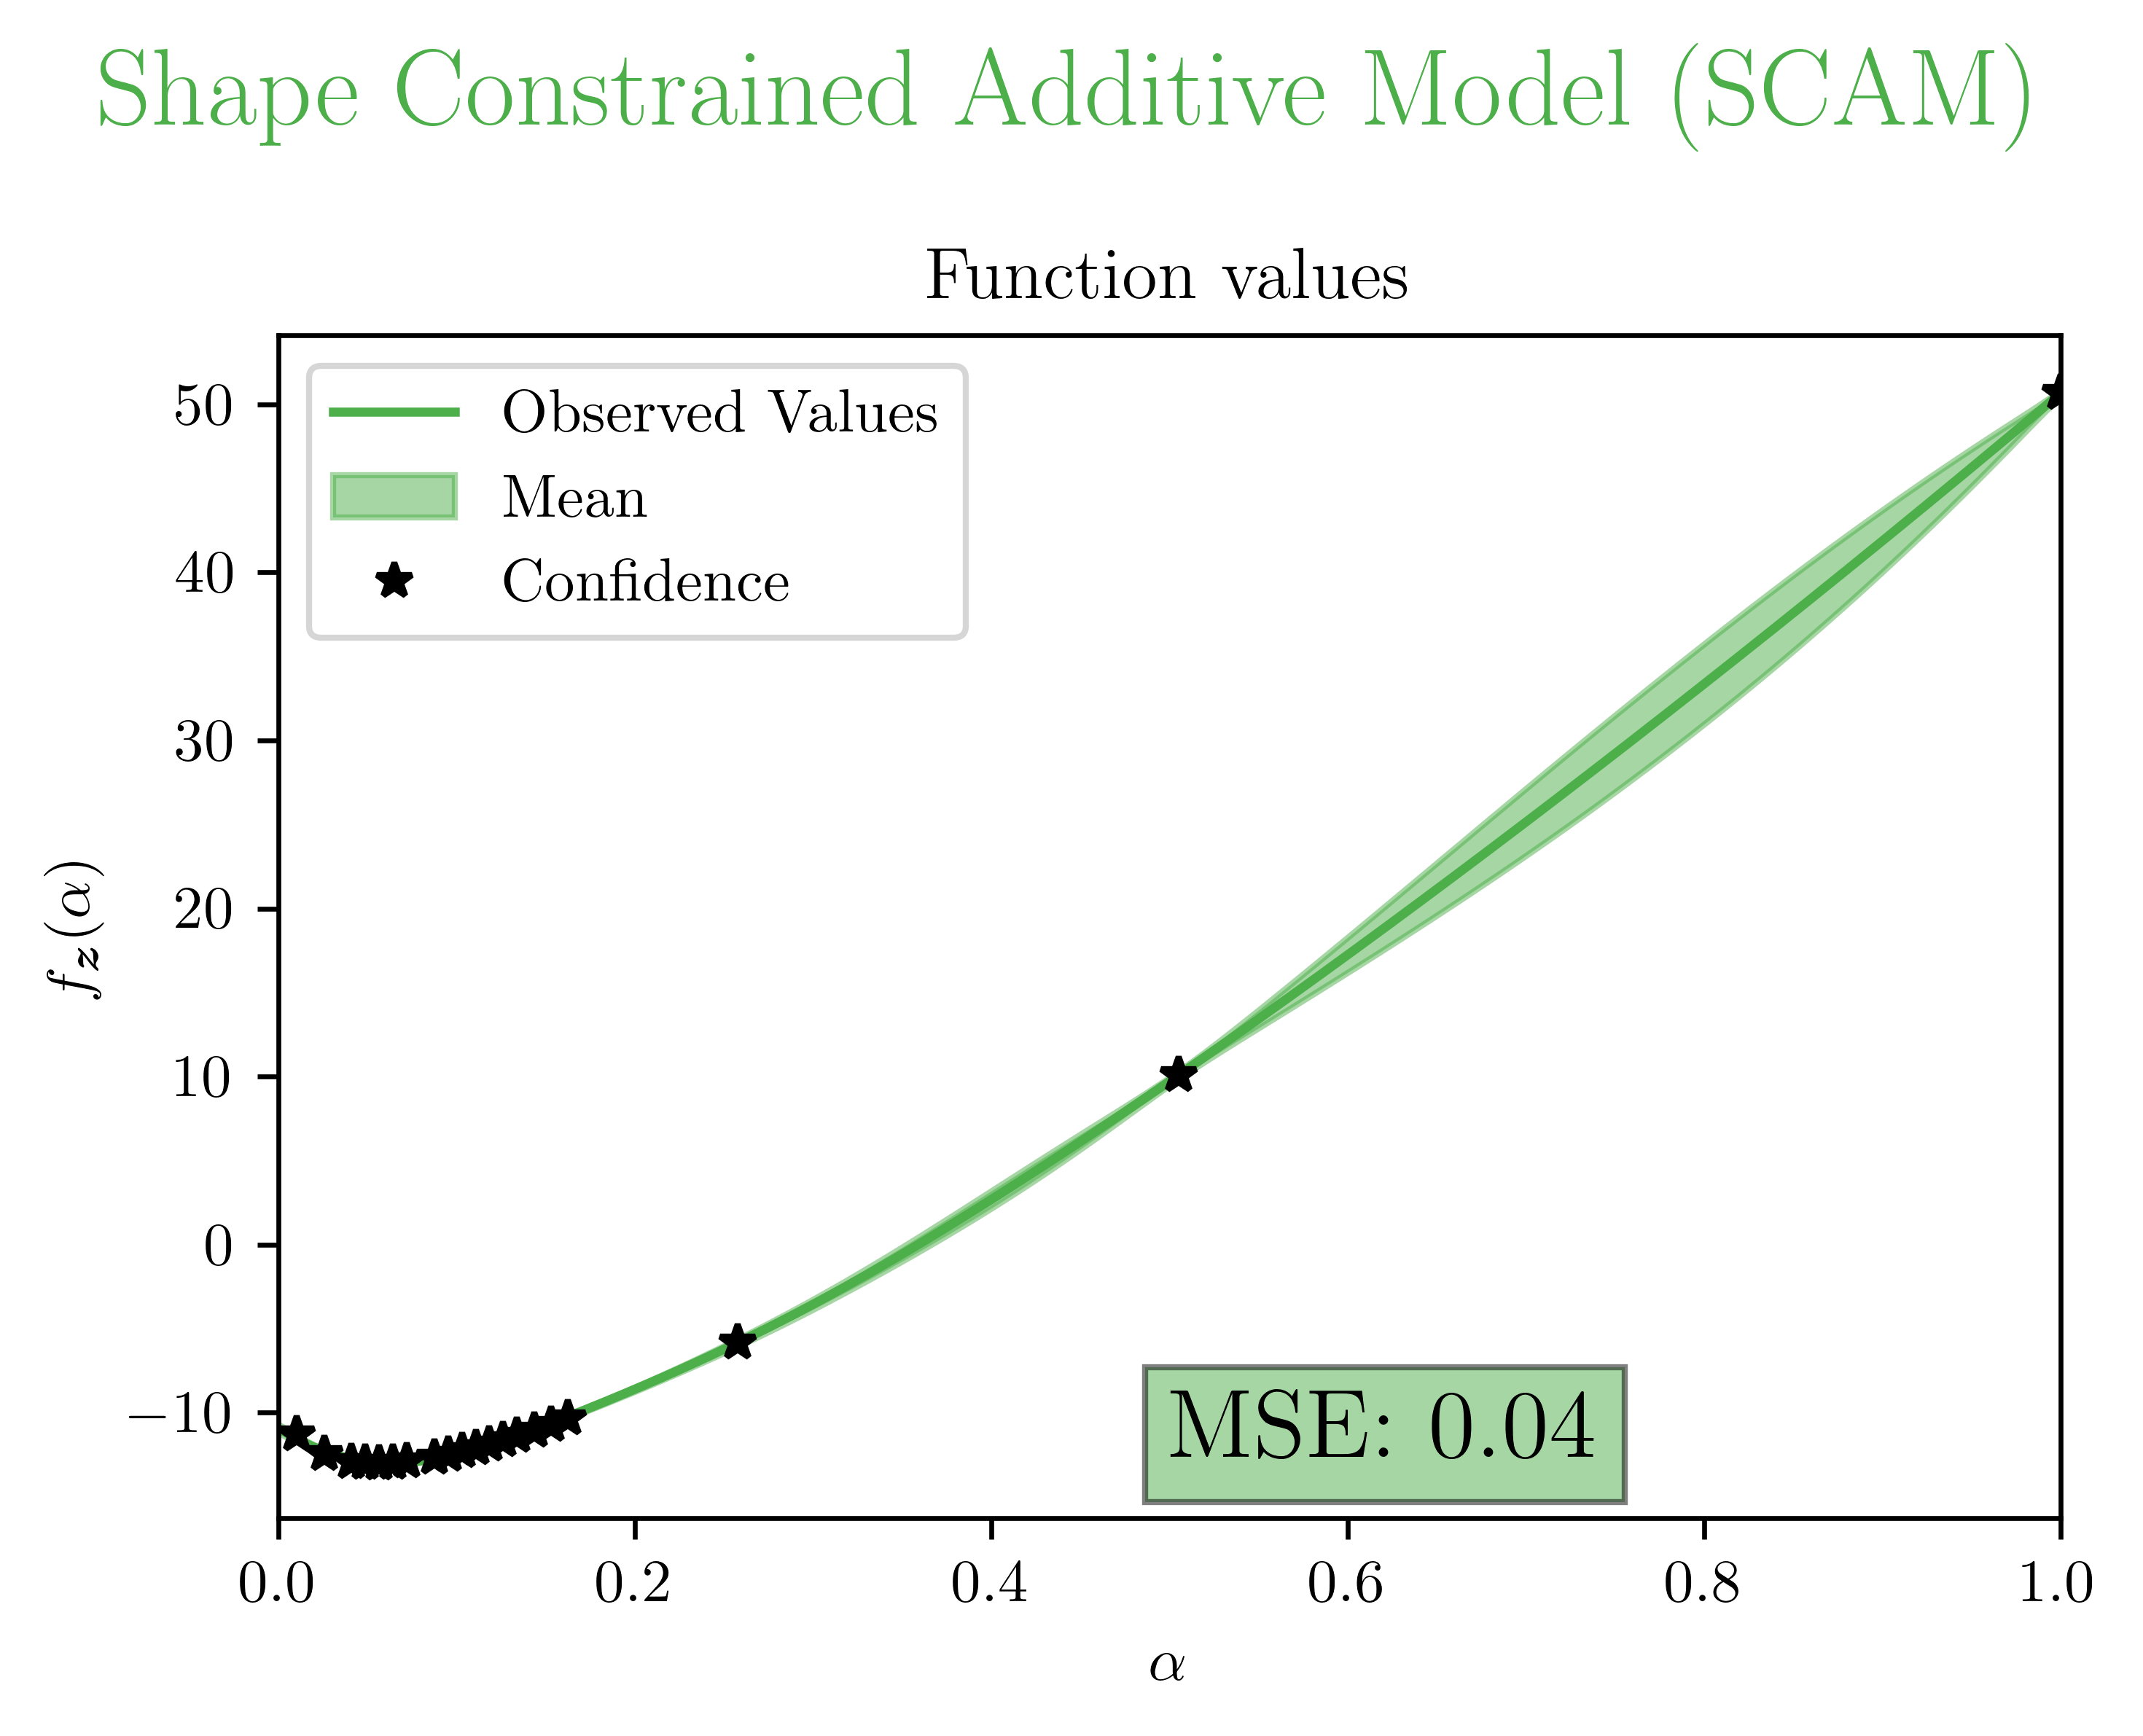
\includegraphics[width=.33\textwidth]{../experiments/adaptive_new_HC/SCAM_20_nobs.png}
    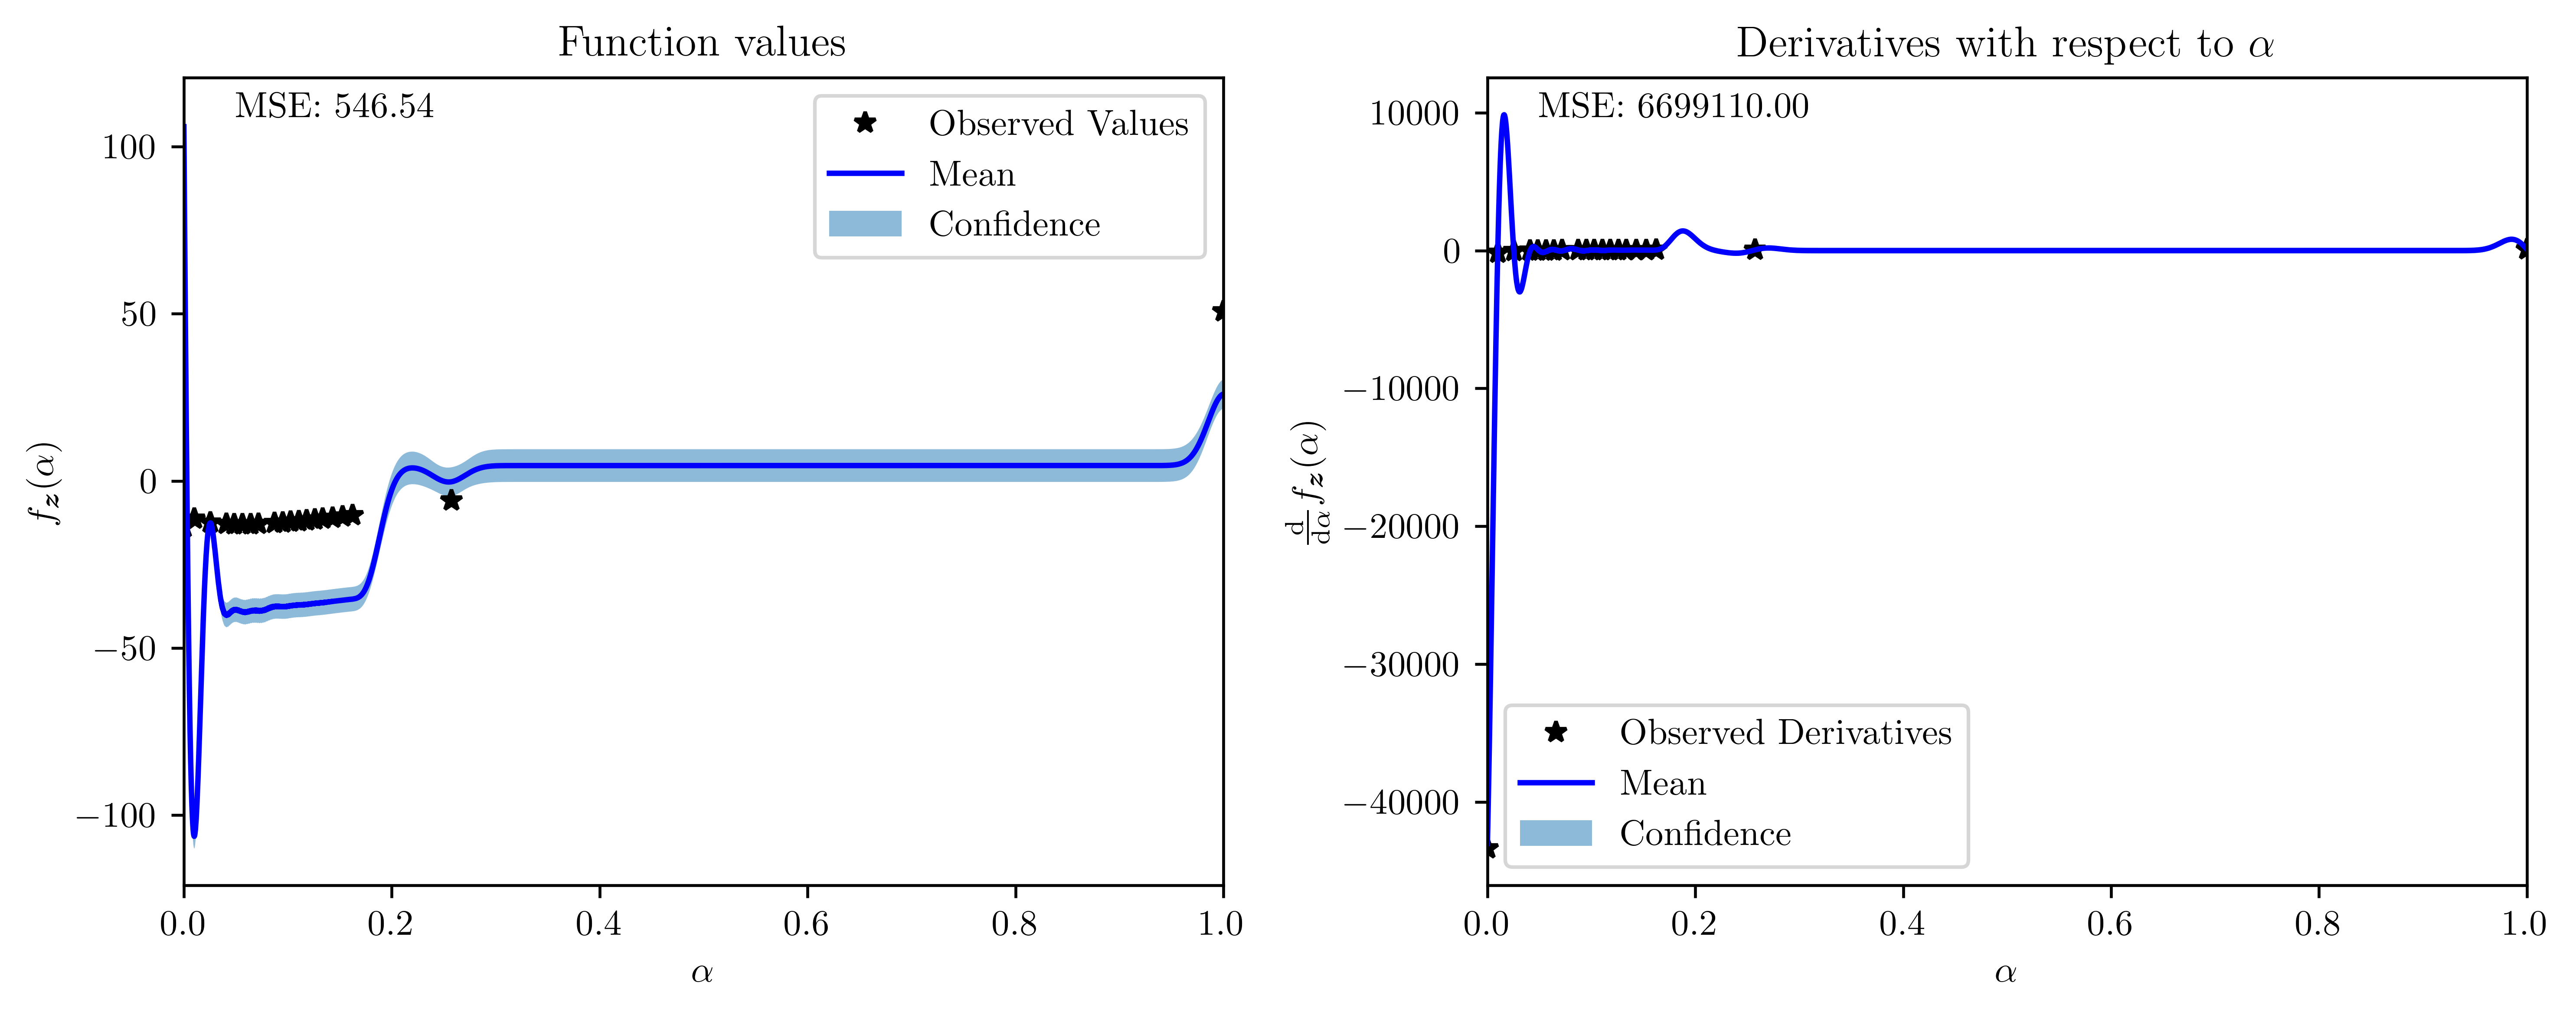
\includegraphics[width=.66\textwidth]{../experiments/adaptive_new_HC/SCGP_20_nobs.png}
    \caption{ {\small Comparison between SCAM and SCGP under high curvature and irregular grid evaluation. Source: author.}}
    \label{fig:SCAMadaptiveHC}
\end{figure}

In scenarios where the SCGP fails to capture the curvature of the function \( f_{\bfz}(\alpha) \), the SCAM still provides a satisfactory fit, as observed in \zcref{fig:SCAMadaptiveHC}.

\subsubsection{Reducing the Number of Observed Points}

Our final experiment consists of replicating the experiment from \zcref{sec:reducingMC}, but comparing the SCGP with the SCAM. However, there is an interesting detail: the SCAM is unable to fit the function \( f_{\bfz}(\alpha) \) with fewer than 10 observed points, which poses a problem in scenarios where the number of evaluations is limited. Furthermore, as seen in \zcref{fig:SCAM10nobs}, the SCAM is able to capture the curvature of the function \( f_{\bfz}(\alpha) \) with 10 observed points, while the SCGP provides an unsatisfactory fit.

\begin{figure}[H]
    \centering
    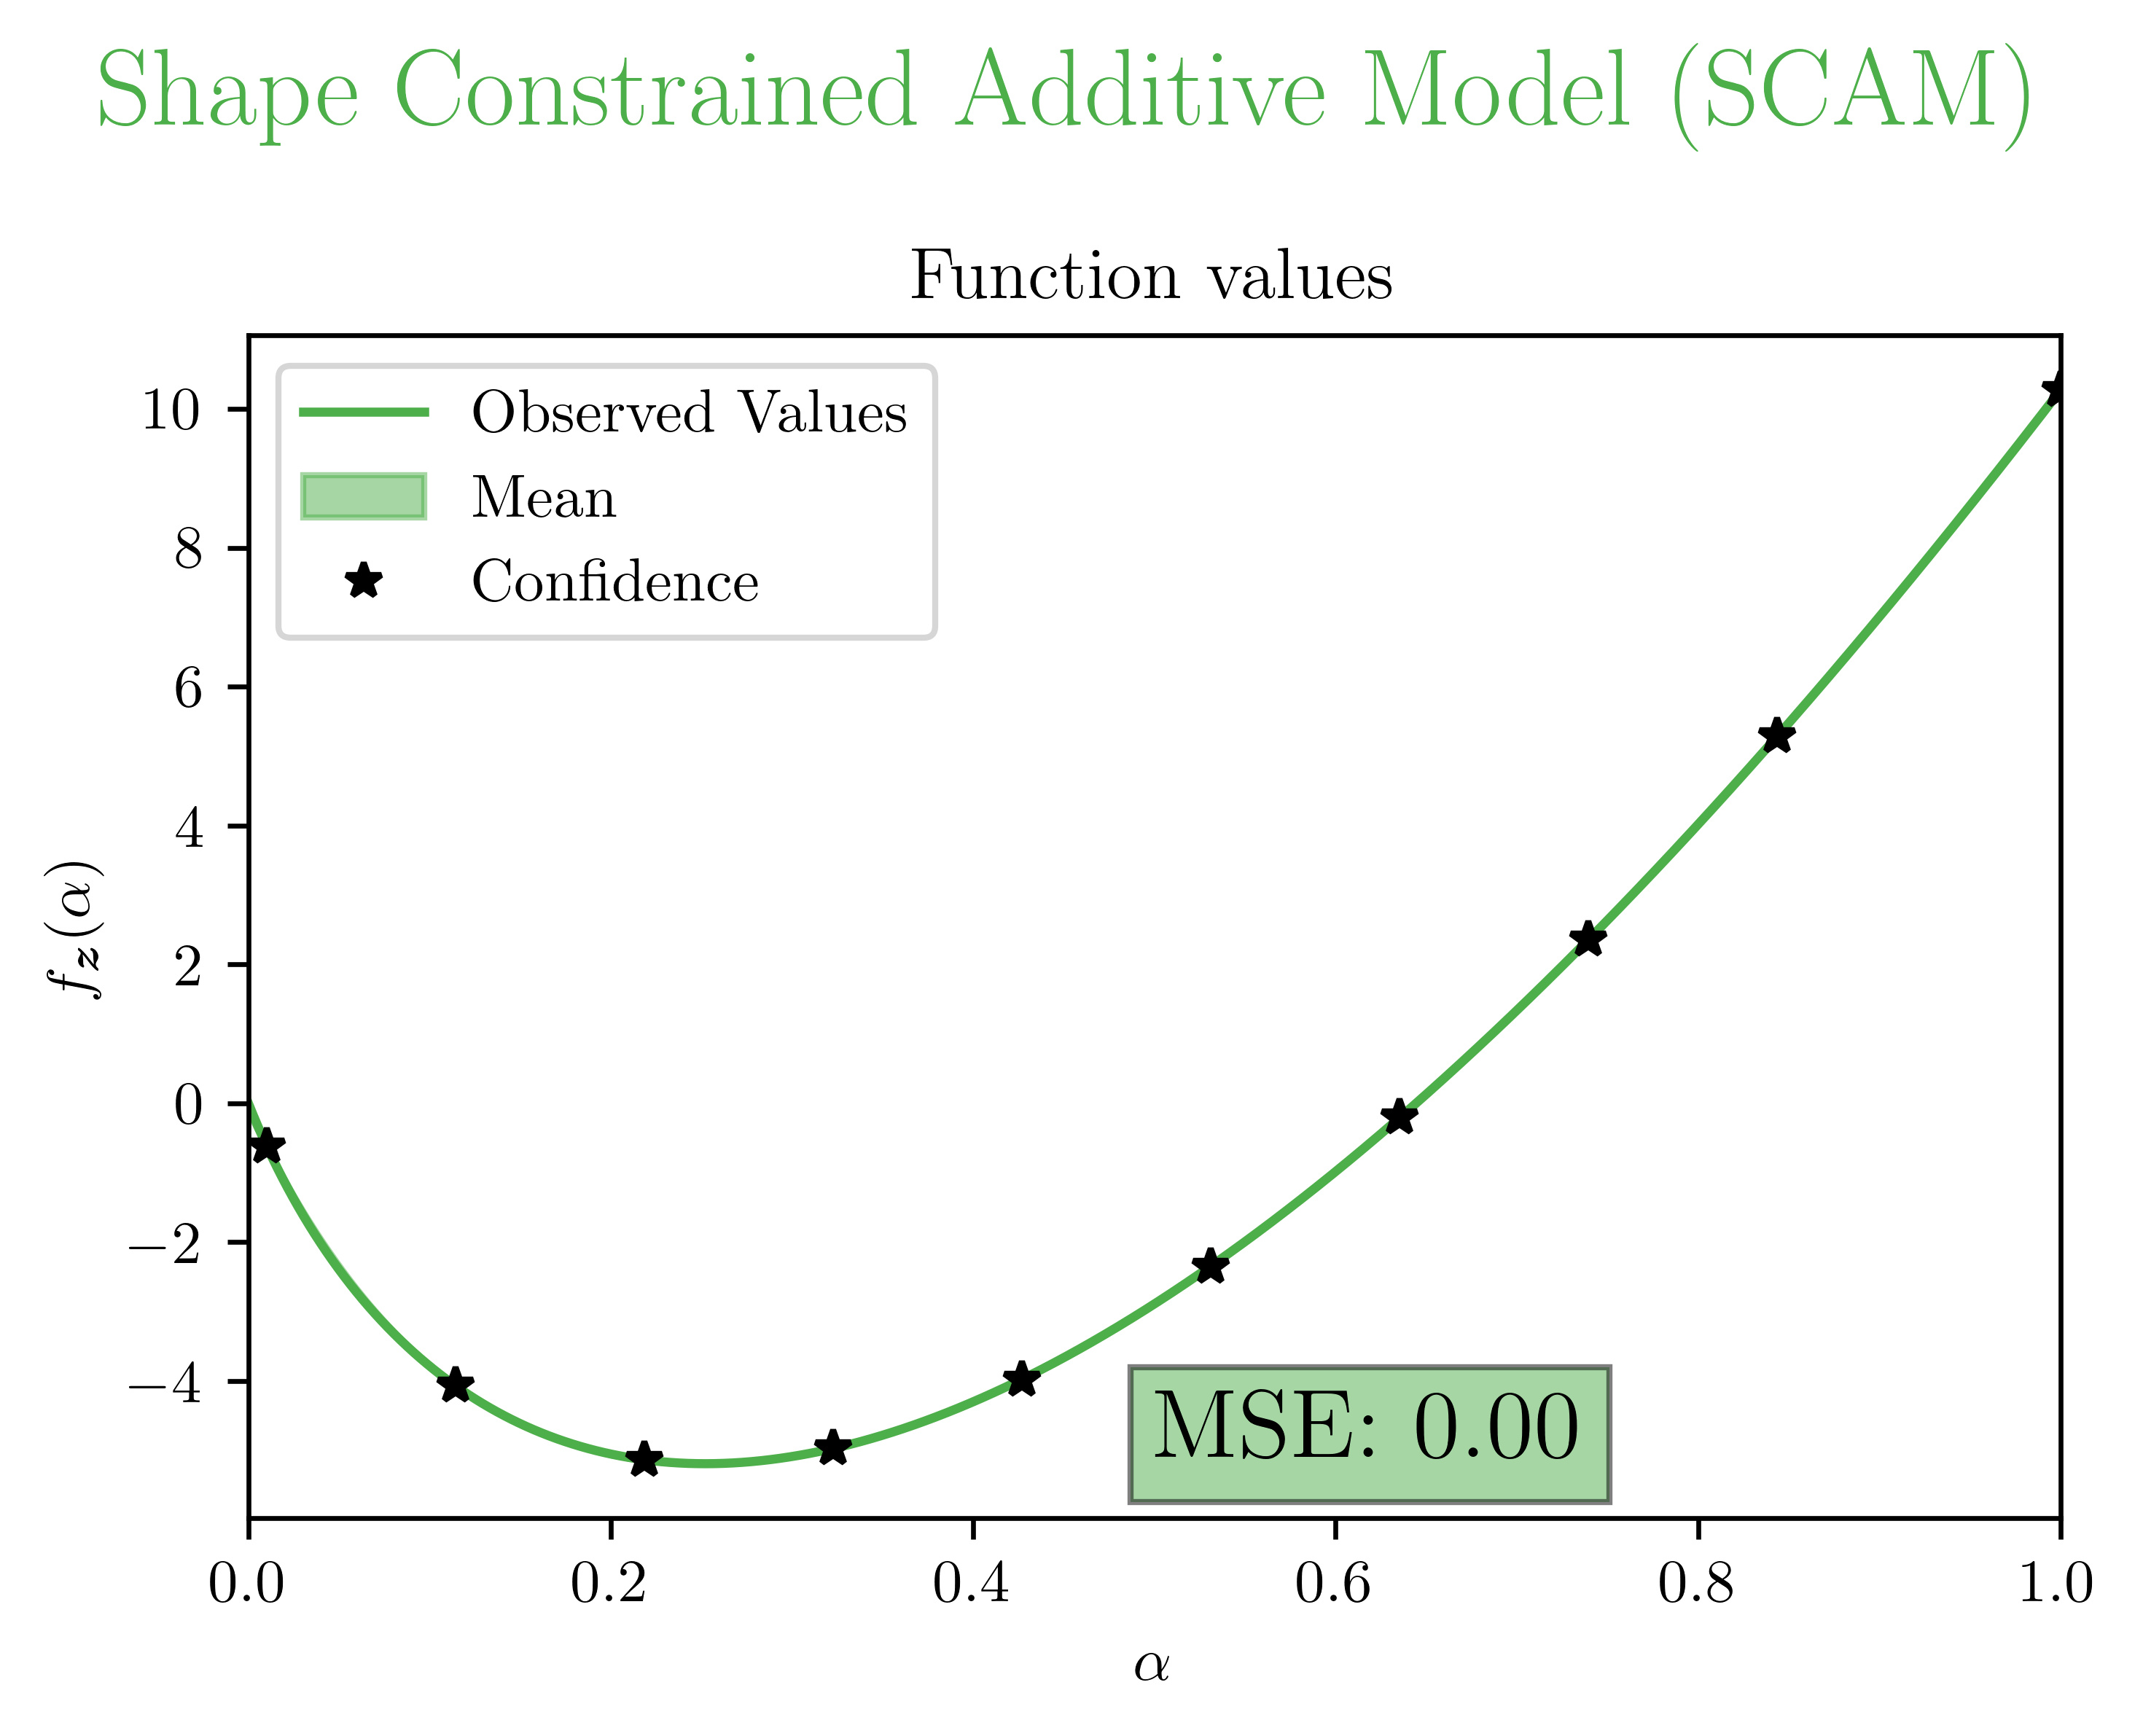
\includegraphics[width=.33\textwidth]{../experiments/uniform_new_MC/SCAM_10_nobs.png}
    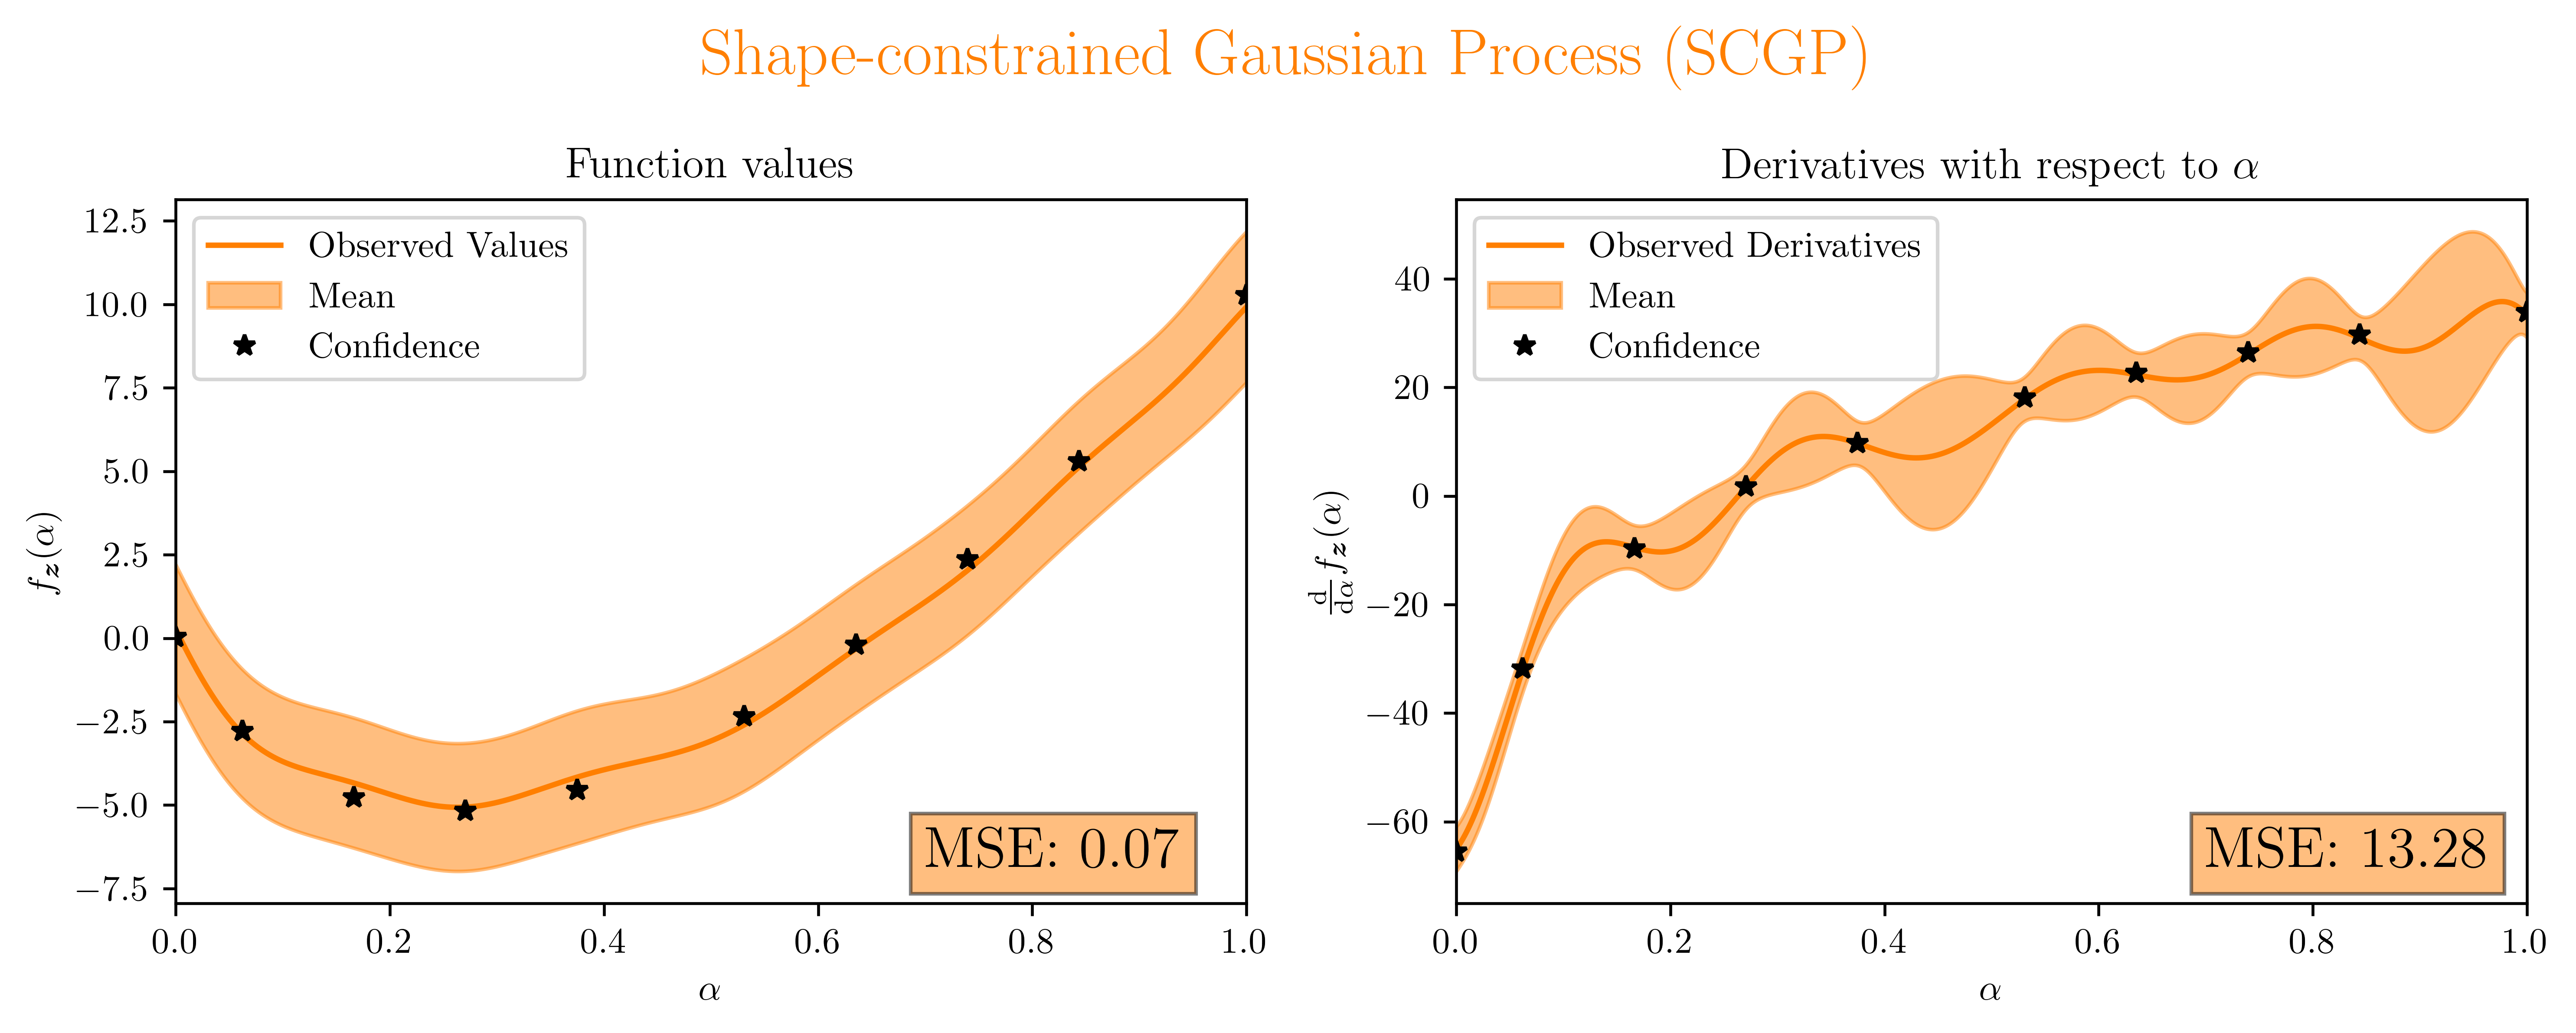
\includegraphics[width=.66\textwidth]{../experiments/uniform_new_MC/SCGP_10_nobs.png}
    \caption{ {\small Comparison between SCAM and SCGP under medium curvature and regular grid evaluation with 10 observations. Source: author.}}
    \label{fig:SCAM10nobs}
\end{figure}
